

%\newif\ifpdf \ifx\pdfoutput\undefined
%\pdffalse % we are not running pdflatex
%\else
%\pdfoutput=1 % we are running pdflatex
%\pdfcompresslevel=9 % compression level for text and image;
%\pdftrue
%\fi

\documentclass[12pt,titlepage,a4paper] {book}
\pagestyle{headings}
\usepackage[latin1]{inputenc}
\usepackage[ngerman]{babel}
\usepackage[T1]{fontenc}
\usepackage{ifpdf}
\usepackage{url}
\usepackage{stmaryrd}
\usepackage{longtable}
%\usepackage[cspex,bbgreekl]{mathbbol}
\usepackage{amsmath,amssymb,latexsym}
\usepackage{bbm}
\usepackage{pslatex}
%\usepackage{graphicx}
\usepackage[bottom,marginal]{footmisc}
\usepackage{setspace}
\usepackage{vmargin}
\usepackage{mathrsfs}

\usepackage{pstricks}
\usepackage{tweaklist}
\renewcommand{\itemhook}{\addtolength{\itemsep}{-2.2mm}
\setlength{\topsep}{0.4ex plus0.2ex minus0.2ex}}

\usepackage{algorithmic}  

\ifpdf
\usepackage[pdftex,xdvi]{graphicx}
\usepackage{makeidx,xspace}
\usepackage{hyperref}
\hypersetup{ 
pdftitle={Kombinatorische Polynomielle Optimierungsalgorithmen},
pdfauthor={Hartmut Wahl},
colorlinks=true,
linkcolor=black,
urlcolor=blue,
hyperindex=true,
pdftex=true,
bookmarksopen=true,
bookmarksopenlevel=0,
bookmarksnumbered=true
}
%\usepackage[pdftex]{color} 
\else
\usepackage[dvips,xdvi]{graphicx}
\usepackage[hyperindex]{hyperref}
%\usepackage{color} 
\fi




%\setpapersize{USletter}
%\setmargins{2.8cm}{1.1cm}% % linker & oberer Rand
%             {16cm}{23.5cm}%   % Textbreite und -hoehe
%             {12pt}{25pt}%   % Kopfzeilenhoehe und -abstand
%             {0pt}{30pt}%    % \footheight (egal) und Fusszeilenabstand

%\usepackage{atbeginend}

%\AfterBegin{itemize}{\setlength{\itemsep}{-2pt} }


%\renewcommand{\familydefault}{ppl}

\parskip5pt plus3pt
\parindent0pt
%\doublespace      
\linespread{1.2}
%\onehalfspacing  
\title{Polynomielle Kombinatorische Optimierungsalgorithmen}
\author{Hartmut Wahl}
%\setcounter{tocdepth}{4}
%\setcounter{secnumdepth}{4}
\usepackage{textcomp}


\def\abstractname{Hinweise}
\newcommand{\RR}{\mathbb{R}}
\newcommand{\NN}{\mathbb{N}}
\newcommand{\ZZ}{\mathbb{Z}}

\newcommand{\vect}[1]{\left(\begin{array}{r} #1 \end{array}\right)}
\newcommand{\mat}[2]{\left(\begin{array}{#1} #2 \end{array}\right)}
\newcommand{\bc}{\bar{c}}

%\newcommand{\entspricht}{\stackrel{\scriptscriptstyle\wedge}{=}}
\newcommand{\entspricht}{\; \hat{=}\; }
\newcommand{\wout}{\;\backslash\;}

%Hack um case f�r algorithmic zu haben
\newenvironment{ALC@case}{\begin{ALC@g}}{\end{ALC@g}}

\newcommand{\CASE}[1]{\item\textbf{case} #1 %
\begin{ALC@case}}
\newcommand{\ENDCASE}{\end{ALC@case}}

%\selectlanguage{USenglish}
\begin{document}
\begin{titlepage}
\ifpdf
\pdfbookmark[0]{Titelseite}{beg}%
\fi
\begin{singlespacing}
\begin{tabular}{l}
{\Large Universit�t zu K�ln}\\

\vspace{9cm}\\


{\bf \large Polynomielle Kombinatorische Optimierungsalgorithmen }\\
Mitschrift der Vorlesung von Prof. M. J�nger\\
WS 2002/2003
\\
\vspace{9cm}
\\
Hartmut Wahl\\
hwahl (at) hwahl (dot) de\\
\vspace{7mm}\\

\end{tabular}
\end{singlespacing}
\end{titlepage}

\pagenumbering{Roman}

%\begin{abstract}
Diese Mitschrift wurde von angefertigt, um mir das Lernen des Stoffes zu
erleichtern und ist keine offizielle Mitschrift des Lehrstuhls. Sie ist
nicht fehlerkorrigiert und sollte mit einer geh�rigen Portion Misstrauen
genossen werden. Korrekturen und Anregungen bitte an mich.

Ich habe beim Lernen noch einige Fehler entdeckt und korrigiert aber 
�bernehme keine Garantie f�r Richtigkeit: Wer eine Garantie will kaufe
sich einen Toaster!

Wer kleine Korrekurvorschl�ge hat, kann sie mir gerne schicken. Wenn jemand
noch gr��ere �nderungen hat (z.B. ein Stichwortverzeichnis w�re fein) kann
ich auch gerne den \LaTeX--Code und die Grafiken zur Verf�gung stellen.
Allerding ist dies mein erstes Dokument mit solchen Umfang in \LaTeX, der
Code mag einem Profi etwas unbeholfen und umst�ndlich vorkommen.

Literatur:\\
Prof. J�nger wies auf dem Semesterapparat hin, der sich in der Bibliothek
der Informatik im Polighaus befindet in dem sich ein Buch befindet:\\
{ Willam J. Cook, William H. Cunningham, William R. Pulleyblank, 
Alexander \mbox{Schrijver}} "`Combinatorial Optimization"', New York: Wiley 1998.\\
Dieses Buch umfasst einen Gro�teil des Stoffes der Vorlesung.\\ Anders als
im Buch angegeben befindet sich das Erratum unter:\\
\url{http://www.math.uwaterloo.ca/~whcunnin/bookpage.html}
%http://www.math.uwaterloo.ca/$\sim$whcunnin/bookpage.html

Die Homepage der Vorlesung ist:\\
\url{
http://www.informatik.uni-koeln.de/ls_juenger/people/liers/Poly/index.html}
%\end{abstract}


\ifpdf
\pdfbookmark[0]{Inhaltsverzeichnis}{index}%
\fi
\begin{onehalfspacing}
\tableofcontents
\end{onehalfspacing}
\pagebreak
%\listoftables
\pagenumbering{arabic}

%{\sffamily\texteuro}


\setcounter{chapter}{-1}

\newtheorem{satz}{Satz}[chapter]
\newtheorem{lemma}[satz]{Lemma}
\newtheorem{korollar}[satz]{Korollar}


\chapter{Einf�hrung}

{
Vor der Einführung machte Prof. Jünger eine ganz kurze informelle 
Vorstellung der kombinatorischen Optimierung, bei der er uns bat nicht 
mit zuschreiben. Dieser Teil ist deshalb hier nicht wieder gegeben. 

\section{Matrizen Exkurs}

Auf Bitten von Kommilitonen machte Prof. Jünger einen kleinen Exkurs in die
Matrizen--Schreibweise, die er verwendet. 

$A x = b\;$ $A \in \RR^{m\times n}\;$ $b \in \RR^{m}$\\
$A = (a_{i j}) = \left(\begin{array}{ccc}a_{11}&\ldots&a_{1n}\\
\vdots&&\vdots\\a_{m1}&\ldots&a_{m n}\end{array}\right)\;$
 $b=\left(\begin{array}{c}b_{1}\\\vdots\\b_{m}\end{array}\right)$

Matrizen-Multiplikation:\\
$A \in \RR^{m\times k}\;$ $B \in \RR^{k \times n};$ $C \in \RR^{m\times n}$ 

$A \cdot B = C$ läuft dann folgendermaßen:

\begin{equation*} 
c_{i j}= \sum^{k}_{p=1} a_{i p} * b_{pi} \; \; \forall\; {i} \;\;\; \mbox{für alle i
Zeilen}
\end{equation*}

Gleichungssysteme:\\
$A x=b$ dabei ist $x=\left(\begin{array}{c}x_{1}\\x_{2}\\\vdots\\x_{n}\end{array}\right) \in \RR^{n}$
anders geschrieben:
\[
\left(\begin{array}{c}a_{11}\\\vdots\\a_{m1}\end{array}\right)
x_{1}+
\left(\begin{array}{c}a_{12}\\\vdots\\a_{m2}\end{array}\right)
x_{2}+\ldots+
\left(\begin{array}{c}a_{1n}\\\vdots\\a_{m n}\end{array}\right)
x_{n} =
\left(\begin{array}{c}b_{1}\\\vdots\\b_{m}\end{array}\right)
\]

Form mit transponierten Vektoren:\\
$c \in \RR^{n}, \;\; y \in \RR^{m}$
\[\begin{array}{rcl} y^{T}A\ &=& c^{T}\\
y_{1}(a_{11}, \ldots, a_{1n}) + y_{2} (a_{21}, \ldots, a_{2n}), + \ldots +
 y_{m} (a_{m1}, \ldots, a_{m n}) &=& (c_{1}, \ldots c_{n})
\end{array}\]

Multiplikation von Vektoren:\\
$a,\; b \in \RR^{n}$\\

\[ab = \sum^{n}_{i=1} a_{i} b_{i} = (a_{1}, \ldots, a_{n})
\left(\begin{array}{c}b_{1}\\ \vdots\\ b_{n} \end{array}\right)\]
Eigentlich müsste man $a^{T}b$ schreiben, da $a$ ja ein transponierter
Vektor ist. Mathematiker vergessen so etwas aber schon mal gerne, das es ja
ohnehin klar ist... 


\section{Allgemeine Formulierungen von Optimierungsproblemen}

\subsection{Generisches Optimierungsproblem}
\begin{tabular}{ll}
Gegeben: & $ A \in \RR^{p \times r},\;  B \in \RR^{p\times r},\; 
C \in \RR^{q\times r}, \; D \in \RR^{q\times s} $\\
& $a \in \RR^{r}, \; b \in \RR^{s}, \; c \in \RR^{p},\; d \in \RR^{q}$\\
(LP)&$\max a^{T}x + b^{T}y$\\
&$A x+ B y = c$\\
&$C x+D y \leq d$\\
&$x \geq 0$\\
\end{tabular}\\

Dies ist die allgemeine Formulierung eines (linearen) generischen
Optimierungsproblems. Für ein ganzzahliges Optimierungsproblem (IP) gilt
zusätzlich zum LP noch:

\[x \in \ZZ^{r}, \;y \in \ZZ^{s} \]

Ein gemischt ganzzahliges Optimierungsproblem liegt vor wenn nur Teile
der Vektoren x und y integral (ganzzahlig) sind.


\subsection{Kombinatorisches Optimierungsproblem}

\begin{tabular}{ll}
Gegeben:& $E$ eine endliche Grundmenge\\
&$y \subseteqq 2^{E},\;$ y ist eine zulässige Teilmenge von $E$\\
&$c$: $E \rightarrow \RR$ (z.b. Zuweisung von Entfernungen zu den
Kanten)\\
&Für $F \subseteqq E$: $c(F) = \displaystyle \sum_{e\in F} c(e)$\\
Gesucht:& $I^{\star} \in  y$ mit $c(I^{\star}) \geqq c(I),\;$ für alle $I \in
 y$\\
\hspace{3mm} oder:&$I^{\star} \in  y$ mit $c(I^{\star}) \leqq c(I),\;$ für
alle $I \in  y$
\end{tabular}


\subsubsection{Kleine Aufwärmaufgabe}

Für $A \in \RR^{m\times n}, \; b \in \RR^{m}$ gilt:\\
($\exists x \in \RR^{n}$) $\;A x = b$ (Gleichungssystem ist lösbar)\\
genau dann wenn:\\
($\nexists y \in \RR^{m}$) $\;y^{T}A=0$, $\;y^{T} b=-1$

Hiernach erklärte Prof. Jünger noch kurz und informell die Triangulation
für Input-/Outputmodelle. In der Nächsten Stunde wurden zunächst 
Reihenfolgeprobleme mit einigen Beispielen im Graphenzeichnen und in der 
Flugplanung veranschaulicht.

\section{Einführung in die lineare Optimierung}

Es folgt ein Beispiel aus der Ölraffinierung: Beim Prozess des so genannten
"`Crackens"' wird Rohöl in drei Produkte aufgespalten: Schweres Öl (S),
mittelschweres Öl (M) und leichtes Öl (L). Nun gibt es zwei verschiedene
Crack-Prozesse die zu einer unterschiedlichen Aufteilung der Endprodukte
führen.

\[\mbox{Prozess 1: 10 ME (= Mengeneinheiten) Rohöl ergibt} \longrightarrow 
\left. \begin{array}{l}
\mbox{2 ME S}\\
\mbox{2 ME M}\\
\mbox{1 ME L}\\
\end{array}\right\} \mbox{Kosten 3 GE}\]

\[\mbox{Prozess 1: 10 ME (= Mengeneinheiten) Rohöl ergibt} \longrightarrow
\left.
\begin{array}{l}
\mbox{1 ME S}\\
\mbox{2 ME M}\\
\mbox{4 ME L}\\
\end{array}\right\}\mbox{Kosten 5 GE}\]

Die Firma hat Lieferverpflichtungen, deswegen muss sie mindestens 3 ME S, 5
ME M und 4 ME L produzieren.

\[\begin{array}{ll}
\mbox{Variablen:}& x_{1}\mbox{, Produktionsniveau von Crackprozess 1}\\
&x_{2}\mbox{, Produktionsniveau von Crackprozess 2}\\
&x_{1}\geqq 0, x_{2}\geqq 0\\
&\mbox{z.B. }x_{1} = 1,5 \L\Leftrightarrow \mbox{ 15 ME Rohöl für Prozess 1}
\end{array}\]

Damit erhalten wir das folgende lineare Optimierungsproblem:\\
\[\begin{array}{l}
\min\; 3x_{1}+5x_{2} \;\;\; \mbox{(Zielfunktion)}\\
\left.\begin{array}{l}\mbox{s.t.}\begin{array}[t]{rl}
(1)& 2x_{1} + x_{2} \geqq 3\\
(2)&2x_{1}+ 2x_{2} \geqq 5\\
(3)&x_{1}+ 4x_{2} \geqq 4\\
(4)&x_{1} \geqq 0\\
(5)&x_{2} \geqq 0\\
\end{array}\end{array}\right\}\mbox{Restriktionen}\end{array}
\]

Jeder Vektor {\scriptsize$\left(\begin{array}{c}x_{1}\\x_{2}\end{array}\right)$} $\in \RR^{2}$, der
(1), (2)...., (5) erfüllt heißt zulässige Lösung.

Graphische Darstellung (gerade keine Lust auf xfig, das bekommt ihr ja wohl
selber hin :)

Aus der n.v. Grafik kann man ganz einfach die optimale Lösung erkennen:
$x^{*} = \mbox{\scriptsize
$\left(\begin{array}{c}2\\0,5\end{array}\right)$}, Wert = 8,5$.

Nähme man nun aber eine beliebige Zielfunktion $a x_{1}+b x_{2}$ sowie $a < 0$ 
und definiere eine Folge von Punkten $x^{(n)}= \mbox{\scriptsize$\left(
\begin{array}{c}n\\ 0\end{array}\right)$}$ mit $n \geq 4$. Weiterhin gilt: 
$a x_{1}^{(n)} + b x_{2}^{(n)} =  n a$. Da a negativ 
ist ist der Wert der Zielfunktion offensichtlich nicht nach unten
beschränkt.

\subsection{Lösungen für Lineare Probleme}

\subsubsection{Simpler Lösungsalgorithmus für ein LP}  

Zunächst stellen wir eine Vermutung an. Wenn eine Optimallösung
existiert, so existiert eine die im Durchschnitt von n Hyperebenen liegt
(wird später bewiesen). Eine Hyperebene ist ein (n-1)-dimensionaler
Unterraum also im $R^{2}$ eine Gerade im $R^{3}$ eine Ebene, u.s.w.

Davon ausgehend konstruieren wie eine einfache Lösungsmethode. Man
schreibe (1), (2), ..., (5) als Gleichungen und löse alle ${5\choose 2}
= 10$ Gleichungssysteme mit 2 Gleichungen. Von allen Lösungen, die
zulässig sind, ist die mit dem kleinsten Zielfunktionswert optimal.

{\bf Aufwand:} Benötigen ${m\choose n}$ Aufrufe des Gleichungssytemlösers mit
n Variablen und n Gleichungen. $\rightarrow$ Viel zu langsam in der
Praxis.

\subsubsection{Idee des Simplexalgorithmus}

Der Simplexalgorithmus geht folgendermaßen vor:\\
(a) Finde eine erste Lösung wie im simplen Algorithmus.\\
(b) Gehe durch Austausch je einer Hyperebene zu einer benachbarten
Lösung deren Zielfunktionswertes nicht schlechter ist.
(c) Wiederhole (b) bis Optimalität festgestellt ist. ($\rightarrow$ via
Dualitätstheorie, die später noch behandelt wird).

\subsubsection{Bestimmung von Schranken}

Wir zeigen nun, dass $x^{*} =
\mbox{\scriptsize$\left(\begin{array}{c}2\\0,5\end{array}\right)$}$ optimal
ist:\\
{\bf Beobachtung 1:} Die Lösungsmenge einer Ungleichung ist invariant
unter Skalierung mit positiven Skalaren, z.B. (1):
\[\{x|2x_{1}+x_{2} \geqq 3\} = \{x|4x_{1}+2x_{2} \geqq 6\}\]

Negative Faktoren kehren die Ungleichung um.

{\bf Beobachtung 2:} Erfüllt ein Vektor zwei gleich gerichtete (beide
"`$\leqq$"' oder beide "`$\geqq$"') so auch die Summe der beiden
Ungleichungen. z.B. (1) + (3):
\[\begin{array}{llcl}
(1)&2x_{1}+x_{2} &\geqq& 3\\
(3)&x_{1}+4x_{2}&\geqq&4\\
\hline
&\underbrace{3x_{1} + 5x_{2}}_{ZF}&\geqq& 7
\end{array}\] 

Nun können wir behaupten, dass wir mindestens 7 GE ausgeben müssen.
$\rightarrow$ Jeder Vektor der (1)...(5) erfüllt hat einen ZF-Wert von
wenigstens 7. Also ist 7 eine untere Schranke für das Minimum. Nun versuchen
wir eine bessere Schranke zu finden:
\[\begin{array}{llcl}
(1)&2x_{1}+x_{2} &\geqq& 3\\
(2)&2x_{1}+2x_{2}&\geqq&5\\
\hline
&4x_{1} + 3x_{2}&\geqq& 8
\end{array}\]
In dieser Ungleichung ist der Koeffizient für $x_{1} = 4$  und ist damit
größer als der Koeffizient in der Zielfunktion. Damit ist dies Ungleichung
nicht zum Abschätzen einer unteren Schranke geeignet. Also ein erneuter
Versuch indem wir (2) mit 1,5 multiplizieren. Damit erhalten wir:
\[3x_{1}+3x_{2} \geqq 7,5\]

\subsubsection{Dualität}

Zwar haben wir nun eine bessere untere Schranke aber dieser Probier-Ansatz ist
etwas unbefriedigend. Darum nun ein systematischer Ansatz
zum Finden der Faktoren für die Gleichungen um eine Schranke zu finden. Da
die Nichtnegativ-Bedingungen in diesem Fall irrelevant sind suchen wir für
unser Problem drei Multiplikatoren ($y_{1}$, $y_{2}$, $y_{3}$) für die
Gleichungen (1) (2) (3).
\[\begin{array}{l}\max \; 3y_{1} + 5y_{2} + 4y_{3} \rightarrow \mbox{Die Rechte
Seite (Schranke) maximieren)}\\
\left.\begin{array}{l}\mbox{s.t.}\begin{array}[t]{lcl}
2y_{1}+2y_{2}+y_{3} &\leqq & 3 \\
y_{1}+2y_{2}+4y_{3} &\leqq & 5
\end{array} \end{array} \right\}\mbox{Damit die ZF-Koeffizienten nicht
überschritten werden}\end{array}\]
Damit haben wir nun das entsprechende duale Optimierungsproblem. Nach
dessen Konstruktion liefert der Zielfunktionswert jeder zulässigen Lösung
des dualen Problems eine untere Schranke für den Zielfunktionswert des
primalen Problems. Wir betrachten:
\[y^{*}=\left(\begin{array}{c}y^{*}_{1}\\y^{*}_{2}\\y^{*}_{3}\end{array}\right)
=\left(\begin{array}{c}0\\\frac{7}{6}\\\frac{2}{3}\end{array}\right)\] 
dies entspricht:
\[\begin{array}{llcl}
\frac{7}{6} \cdot (2):\; & \frac{14}{6}x_{1} + \frac{14}{6}x_{2} &\geqq&
\frac{35}{6}\\
\frac{2}{3} \cdot (3):\; & \frac{4}{6}x_{1} + \frac{16}{6}x_{2} &\geqq&
\frac{16}{6}\\
\hline
&3x_{1} + 5x_{2} &\geqq& 8,5
\end{array}
\]

\paragraph{Schwacher Dualitätssatz}
Es seien $c \in \RR^{n}$, $b \in \RR^{m}$, $A \in \RR^{m \times n}$ für die
Optimierungsaufgaben:

\begin{tabular}{ll}
(P)&$\min \{c^{T}x | A x \geqq b, \; x\geqq 0\}$\\
&d.h. bestimme $x^{*} \in \RR$ mit $A x^{*} \geqq b$, $x^{*} \geqq 0 $ und
$c^{T}x^{*}$ so klein wie möglich.\\
(D)&$\max \{y^{T}b|y^{T}A \leqq c^{T}, \; y \geqq 0\}$\\
&d.h. bestimme  $y^{*} \in \RR^{m}$ mit $g^{*T}A \leqq c^{T}, \; y ^{*}
\geqq 0$ und $y^{*T}b$ so groß wie möglich.
\end{tabular}

so gilt folgendes: Seien $x_{0} \in \RR^{n}$, $ y_{0} \in \RR^{m}$ Punkte
mit $A x_{0} \geqq b $, $x_{0} \geqq 0$ und $y_{0}^{T}A \leqq c^{T}$,
$y_{0} \geqq 0$ dann gilt $y_{0}^{T}b \leqq c^{T} x_{0}$\\
Beweis:
\[y_{0}^{T}b \leqq y_{0}^{T}(A x_{0}) = (y_{0}^{T}A)x_{0} \leqq c^{T}x_{0}
\; \; \; \; \mbox{q.e.d.}\] 

Der starke Dualitätssatz (später) besagt $y^{*T}b =c^{T}x^{*}$ für
Optimallösung $x^{*}$ von (P) und $y^{*}$ von (D).

\subsubsection{Ökonomische Interpretation des Dualen Programms}

Ein Manager der Ölraffinerie würde sich nun die Frage stellen, ob es sinnvoll
L, M uns S selbst herzustellen, oder ob man es auf dem Markt kaufen sollte 
b.z.w.  bei welchen Marktpreis eine Produktion nicht mehr lohnt. In diesem Fall
drückt $y_{1}$ den Preis in GE für S aus, $y_{2}$ für M, $y_{3}$ für L. Der
Marktpreis für die benötigten Mengen beträgt somit:
\[3y_{1} + 5y_{5} + 4y_{3} \; \; \mbox{GE}\]
der Ausstoß von Crackprozess 1 hat den Marktpreis:
\[2y_{1}+2y_{2}+3y_{3} \; \; \mbox{GE} > 3 \;\;\;\; \rightarrow \mbox{Produktion Lohnt}\]
der Ausstoß von Crackprozess 2 hat den Marktpreis:
\[y_{1}+2y_{2}+4y_{3} \;\; \mbox{GE} > 5 \;\;\;\; \rightarrow \mbox{Produktion Lohnt}\]
$y_{i}$ werden auch als Schattenpreise bezeichnet. In unserem Beispiel
betragen sie:
\[\begin{array}{lll}(S):\; y_{1}^{*}=0& (M):\; y_{2}^{*} =
\frac{7}{6}&(L):\;
y_{3}^{*} = \frac{2}{3}
\end{array}\]
Hier ist zu erkennen dass S praktisch "`wertlos"' für die Firma ist. In der
tat ist es in der Optimallösung im Überfluss vorhanden (also mehr als die
Lieferverpflichtungen der Firma verlangen. D.h. man würde das Öl zunächst
zu jedem Preis verkaufen (solange man die insgesamte Produktionsmenge
dadurch nicht erhöhen muss).

\subsection{Formen von Linearen Problemen \label{FormenLP}}

\subsubsection{Kanonische Form eines LPs}

Die Kanonische Form eines LPs lautet:
\[\begin{array}{lcl}
\max\; c^{T}x\\
A x&\leqq& b\\
x&\geqq& 0
\end{array}\]
Transformationen von anderen Standardformen in die kanonische Form:
\[\begin{array}{l@{\hspace{3mm}}rcl@{\hspace{8mm}}c@{\hspace{8mm}}rcl}
1)&\max  a^{T}y&&&&\max a^{T}x\\
&B y&=&d&\stackrel{x=y}{\longrightarrow}&\mbox{\scriptsize$\left(\begin{array}{r}B\\-B\\\end{array}
\right)$}x&\leqq&\mbox{\scriptsize$\left(\begin{array}{r}d\\-d\end{array}
\right)$}\\
&y&\geqq& 0&&x&\geqq& 0\vspace{5mm}\\
2)&\max a^{T}y&&&&\max \mbox{\scriptsize$\left(\begin{array}{r}a\\-a\end{array}\right)$}^{T}x\vspace{2mm}\\
&B y&\leqq&d&\stackrel{x=\mbox{\scriptsize$\left(\begin{array}{r}y+\\y-\end{array}
\right)$}}{\longrightarrow}&(B, -B)x&\leqq& d\\
&&&&&x&\geqq& 0\vspace{5mm}\\
3)&\max a^{T}y&&&&\max
\mbox{\scriptsize$\left(\begin{array}{r}a\\-a\end{array}\right)$}^{T}x\vspace{2mm}\\
&B y&=&d&\stackrel{x=\mbox{\scriptsize$\left(\begin{array}{r}y+\\y-\end{array}
\right)$}}{\longrightarrow}&   
\mbox{\scriptsize$\left(\begin{array}{rr}B&-B\\-B&B\end{array}\right)$}
x&\leqq& \mbox{\scriptsize$\left(\begin{array}{r}d\\-d\end{array}
\right)$}\\
&&&&&x&\geqq& 0
\end{array}\]
Als Hausaufgabe dürfen wir die Transformationen in die andere Richtung
machen :), (bei $B y=d$ geht es nicht).

Jedes LP kann also auch in die Form $\max \{c^{T}x| A x \leqq b\}$ transformiert
werden.

\paragraph{Farkas Lemma}
Wir suchen ein Analogon zur "`Aufwärmaufgabe"':\\
$A \in \RR^{m\times n}, \; \; b \in \RR^{m}$\\
$(\exists x) \; \;\; A x = b$ genau dann wenn $(\nexists y) \; \; y^{T}A
= 0, \; \; y^{T}b=-1$ für Ungleichungsprobleme der Form $A x\leqq b$


\paragraph{Fourier-Motzkin Elimination}

Durch Multiplikation der Ungleichungen mit positiven Skalaren und Umordnung
erhalten wir:
\[
(*)\left\{\begin{array}{rcl}
x_{1} + (a_{i}')^{T}  x'&\leqq& b^{*}_{i} \;\; \forall \; i\; \in
\{1,2,3,...m'\}\;\;\; \mbox{alle mit pos. Faktor vor $x_1$}\\
-x_{1} + (a_{i}')^{T}  x'&\leqq& b^{*}_{i} \;\; \forall \; i\; \in
\{m'+1,...m''\}\;\;\; \mbox{alle mit neg. Faktor vor $x_1$}\\
(a_{i}')^{T}  x'&\leqq& b^{*}_{i} \;\; \forall \; i\; \in
\{m''+1,...m\}\;\;\; \mbox{hier war gar kein $x_1$ drin}\\
\end{array}\right.
\]
\begin{tabular}{ll}
wobei&$x'=(x_{2}, x_{3},...x_{n})$\\
&$(a_{i}')^{T}$ ist die i-te Zeile von A ohne den ersten Eintrag
\end{tabular}

Die ersten beiden Zeilen von (*) sind äquivalent zu
\[\max_{m'+1\leqq j \leqq m''} \left((a_{j}')^{T} x' -b_{j}\right) \leqq x_{i}
\leqq \min_{1\leqq i \leqq m'} \left(b_{i} - (a_{i}')^{T}x'\right)\]

d.h. das Orginalsystem $A \leqq b$ hat eine Lösung genau dann wenn (in
Zukunft g.d.w.) das System:
\[
(**)\left\{\begin{array}{rcll}
(a_{j}')^{T}x' -b_{j} &\leqq& b_{i} - (a_{i}')^{T}x'& \forall \; i \; \in
\{1,2,3,...m'\}\\
%(a_{j}')^{T}x' -b_{j}&\leqq& b_{i} - (a_{i}')^{T}x'
&&&\forall \; i \; \in
\{m'+1,...m''\}\\
(a_{i}')^{T}x' &\leqq& b_{i}'& \forall \; i \; \in
\{m''+1,...m\}\\
\end{array}\right.
\]
eine Lösung hat ($x_{i}$ kann geeignet gewählt werden).\\
Umformulierung von (**)
\[
(***)\left\{\begin{array}{rcll}
(a_{i}'+a_{j}')^{T} x' &\leqq& b_{i} + b_{j}& \forall \; i \; \in
\{1,2,3,...m'\}\\
%(a_{i}'+a_{j}')^{T} x' &\leqq& b_{i} + b_{j}
&&& \forall \; i \; \in
\{m'+1,...m''\}\\
(a_{i}')^{T}x' &\leqq& b_{i}'& \forall \; i \; \in
\{m''+1,...m\}\\
\end{array}\right.
\]
Schreibe (***) als $A'x'\leqq b'$\\
Also $(\exists x) \; \; A x\leqq b$ g.d.w. $(\exists x') A' x' \leqq b'$

Fazit: Wir haben die Variable x eliminiert und haben jetzt in (***) $n-1$
Variablen und $m'(m''-m')+m-m''$ Ungleichungen $\rightarrow$ weniger
Variablen aber mehr Ungleichungen.

Diese Iteration liefert ein nicht polynomielles Verfahren zur Lösung von
Ungleichungssystemen.

\begin{lemma}
von Farkas für Ungleichungen\\
Seien $A \in \RR^{m\times n}$, $b\in \RR^{m}$\\
$(\exists x \in \RR^{n})$ $A x \leqq b\;$ g.d.w. $\;(\nexists y \in \RR^{m})$
$y\geqq 0$, $y^{T}A=0$, $y^{T}b < 0$\\
\end{lemma}

\begin{longtable}[l]{lp{13cm}}
\multicolumn{2}{l}{{\bf Beweis}}\\
"`$\Rightarrow$"'&$A x \leqq b$ habe eine Lösung $\bar{x}$\\
&Annahme:  $(\exists y \geqq 0) \; \; y^{T} A = 0, \; \; y^{T}b < 0$\\
&\[\begin{array}{rcl}
\Rightarrow 0 &>& y^{T}b\\
&\geqq & y^{T}A\bar{x}\\
&=& 0\; \; \lightning
\end{array}\]\\
&Mit $0>0$ ergibt sich also ein Widerspruch. Also gilt die Hin-Richtung.\\
"`$\Leftarrow$"'& $A x \leqq b$ habe keine Lösung.\\
& 1) Induktionsverankerung: $A \in \RR^{m\times 1}$
Nach Skalierung mit positiven Skalaren $\bar{y}$ haben alle Ungleichungen
die Form:\\
&\[(1) \; \; \; x_{n} \leqq \alpha ;\ \; \; \mbox{ oder } (2) \; \; \; 
-x_{n} \leqq \beta\]\\
&Nicht Lösbarkeit bedeutet also dass sich zwei Ungleichungen widersprechen.
O.b.d.A (=Ohne Beschränkung der Allgemeinheit) widersprechen sich die i-te 
Form (1) und die (j)-te der Form (2). D.h. $-\beta \leqq x_{n} \leqq \alpha$
mit $\alpha < -\beta$ d.h. $\alpha + \beta = \gamma < 0$\\

&Man wähle nun $\begin{array}[t]{rcl}
y_{i} &=& - \frac{\bar{y}_{i}}{\gamma} > 0 \;\;\; \mbox{ da } \gamma <
0\vspace{2mm}\\
y_{j} &=&- \frac{\bar{y}_{j}}{\gamma} > 0 \vspace{2mm}\\
y_{k} &=& 0 \; \; \; \mbox{ für } k \not\in \{i,j\}
\end{array}$\\
 
&\[\begin{array}{lrcl}
\Rightarrow& y &\geqq& 0\\
& y^{T}A &=& \left(\ldots,0, - \frac{\bar{y}_{i}}{\gamma},0,\ldots,0,
- \frac{\bar{y}_{j}}{\gamma},0,\ldots\right) \left(\begin{array}{c}
\vdots\\\ast\\\frac{1}{y_{i}}\\\ast\\\vdots\\\ast\\-\frac{1}{y_{j}}\\\ast
\\\vdots \end{array}\right)\\
&&=& - \frac{1}{\gamma} + \frac{1}{\gamma} = 0\\
&y^{T}b &=& - \frac{\alpha}{\gamma} - \frac{\beta}{\gamma} = 
- \frac{\alpha + \beta}{\gamma} = -1 < 0
\end{array}\]\\

&2) Induktion: $A \in \RR^{m \times n} \; \; n > 1 $\\
& $A x \leqq b$ hat keine Lösung $\Leftrightarrow A'x \leqq b'$ hat keine Lösung\\
& 3) Induktionsannahme $\begin{array}[t]{rcl}(\exists y' \geqq 0) 
\; \; y'^{T}A' &=& 0\\ y'^{T}b'&=&-1\end{array}$\\
&d.h.  $(\exists y' \geqq 0) y'^{T} [A'b'] =
(\underbrace{0,\ldots,0}_{n-1},-1) $\\
&Jede Zeile der Matrix $[0,\;A',\;b']$ ist Summe von nicht-negativ skalierten
Zeilen von $[A,\; b]$\\
&$\Rightarrow \; (\underbrace{0,\ldots,0}_{n},-1)$ ist nicht-negative
Linearkombination der Zeilen von $[A, \, b]$\\
&d.h. $(\exists y \geqq 0) \;\; y^{T} A = 0\; \; \; \; y^{T}b = -1$
\end{longtable}

\begin{korollar}
Lemma von Farkas, 1894

Seien $A\in \RR^{m\times n}, \; \; b \in \RR^{m}$
\[\begin{array}{rcllrcl}
(\exists x \in \RR^{n}) \; \; x &\geqq& 0 & g.d.w. & (\nexists y \in
\RR^{m}) \; \; y^{T}A &\geqq& 0\\
A x&=&b&&y^{T}b &<& 0
\end{array}\]
\end{korollar}

{\bf Beweis:} Für $\bar{A} = \left(
\begin{array}{c}A\\-A\\-I\end{array}\right)$ (mit $I=$ Einheitsmatrix) und
$\bar{b} = \left( \begin{array}{c}b\\-b\\0\end{array} \right)$ gilt:\\
\[\begin{array}{rcrcl}
(\exists x \geqq 0) \; A x = b &\stackrel{\mbox{\scriptsize Konstruktion}}{\Leftrightarrow}&
(\exists \bar{x}) \; \; \bar{A} \bar{x} &\leqq&\bar{b}\\
&\stackrel{\mbox{\scriptsize Satz 0.1 (Lemma für Ungl.)}}{\Leftrightarrow}&
(\nexists \bar{y} \geqq 0) \; \; \bar{y}^{T} \bar{A} &=&0\\
&&\bar{y}^{T}b&\leqq&0
\end{array}\]
\[\begin{array}{lcrcl}
\left[\bar{y}=\left(\begin{array}{c}u\\v\\w\end{array}\right)\right]
&\Leftrightarrow& \nexists
\left(\begin{array}{c}u\\v\\w\end{array}\right)\geqq 0 \; \; \; \;\;
u^{T}A - v^{T} A - w^{T} &=& 0\\
&&u^{T}b - v^{T} b &<& 0\\\\
\left[ y = u -v\right]&\Leftrightarrow&(\nexists y) \; \; y^{T} A &\geqq&
0\\ &&y^{T}b &<& 0 \hspace{7mm} \mbox{q.e.d}
\end{array}\]


Farkas Lemma kann auch anders betrachtet werden: 
\[\begin{array}{lrclrcl}
\mbox{Entweder}&(\exists x) A x &=& b, & x &\geqq& 0\\
\mbox{oder}&(\exists y) y^{T}A &\geqq& 0, & y^{T}b &<& 0
\end{array}\]
aber nicht beides. Dies kann man im $R^{2}$ auch graphisch darstellen in
dem man die Matrix $A=(A_{1}, A_{2}$ als Zusammensetzung aus zwei 
Vektoren $A_{1}$ und
$A_{2}$ betrachten, die jeweils eine "`halbe"' Ebene beschreiben. $y^{T}A 
\geqq$ beschreibt dann den Schnitt aus diesen beiden "`halben"' Ebenen. 
$y^{T}b < 0$ beschreibt wiederum eine "`halbe"' Ebene. Wenn jetzt nun $A x=b$ 
gelten soll so muss $b$ sich als eine Linearkombination der Vektoren $A_{1}$ 
und $A_{2}$ darstellen lassen. Anschaulich bedeutet dass das $b$ in der 
Zeichnung "`zwischen"' $A_{1}$ und  $A_{2}$ liegen muss dann wiederum wird
sich die Flächen die durch $y^{T}A \geqq 0$ und durch $y^{T}b < 0$
beschrieben werden niemals schneiden. 

Leider habe ich an dieser Stelle nicht die Zeit die Zeichnungen zu malen.
Freiwillige vor.

\begin{korollar} \label{eineLoesung}
Das System $A x \leqq b$ habe wenigstens eine Lösung. Dann erfüllt jede
Lösung $x$ von $A x\leqq b$ die Ungleichung $c^{T}x \leqq \delta$ genau dann,
wenn ein $y\geqq 0$ existiert, so dass $y^{T}A=c^{T}$ und $y^{T}b \leqq
\delta$.

\end{korollar}

Beweis:
\begin{longtable}{lp{13cm}}
"`$\Leftarrow$"'& $(\exists y \geqq 0) y^{T}A = c^{T}, \; \; y^{T}b \leqq
\delta$\\
&für alle $x \in \RR^{n}$ gilt:\\
&\[\begin{array}{r@{\Rightarrow}rcl}
A x \leqq b & y^{T} A x&\leqq& y^{T}b\\
&c^{T}x &\leqq& y^{T}b\\
&c^{T}x &\leqq & \delta
\end{array}\]\\
"`$\Rightarrow$"' & Annahme \\
&\[\begin{array}{rcl}(\nexists y \geqq 0 )y^{T}A&=&
c^{T}\\
y^{T}b \leqq \delta
\end{array}\]\\
&$\Rightarrow (\nexists y \geqq 0, \; \; \lambda \geqq 0)\; \; \;
(y^{T}, \; \lambda) \left(\begin{array}{cc}A&b\\ 0&1\end{array} \right) =
(c^{T},\; \delta)$\\
&$\stackrel{\mbox{\scriptsize (Farkas)}}{\Rightarrow}\begin{array}[t]{l@{\vspace{7mm}}rcl}
\left(\exists \left(\begin{array}{c}z\\\mu\end{array}\right)\right)&
\left(\begin{array}{cc}A&b\\0&1\end{array}\right)
\left(\begin{array}{c}z\\\mu\end{array}\right) &\geqq&0\\
&(c^{T},\; \delta) \left(\begin{array}{c}z\\\mu\end{array}\right) &<&0
\end{array}$
\end{longtable}

Fall 1 $\mu =0$:
\[\Rightarrow \left\{ \begin{array}{rcl}
A z &\geqq & 0\\
c^{T}z&<&0\\
\end{array}\right.\]
Sei $x^{0}$ Lösung von $A x\leqq b$. Für $r$ hinreichend groß gilt dann:
\[\begin{array}{rcl}A(x^{0} -r z) &\leqq& b\\
c^{T}(x^{0}-r z)&>&\delta\end{array}\]
$\bar{X}=x^{0} -r z$ ist Lösung die $c^{T}\bar{x} \leqq \delta$ verletzt.

Fall 2 $\mu > 0$:\\
Es gilt $A z + b \mu \geqq 0$
\[\begin{array}{crcl}
\Rightarrow & A z &\geqq & -b \mu\\
\Rightarrow & A\left(-\frac{z}{\mu} \right)&>& \delta
\end{array}\]
aber $c^{T}z + \delta\mu < 0$
\[\begin{array}{crcl}
\Rightarrow & c^{T}z &<& - \delta \mu \\
\Rightarrow & c^{T}\left(-\frac{z}{\mu}\right) &>& \delta
\end{array}\]

Also liefert die Lösung $\bar{x}=-\frac{z}{\mu}$ den Widerspruch.

\section{Dualitätstheorem}

Für das lineare Optimierungsproblem:
\[(P) \; \; \; \{\max c^{T}x | A x \leqq b\}\]
bezeichnen wir:
\begin{itemize} 
\item Jede Lösung $\bar{x}$ von $A x \leqq b$ als zulässige Lösung
\item Jede zulässige Lösung $\bar{x}$ die $c^{T} x $ maximiert als
Optimallösung.
\end{itemize}
Wir definieren das duale lineare Optimierungsproblem zu (P)
als (D) \[\min \{y^{T}b| y \geqq 0 , \; \; y^{T}A = c^{T} \}\]

\begin{satz} \label{SchwQual} Schwaches Dualitätstheorem\\
Seien $A \in \RR^{m \times n}, \; \; b \in \RR^{m}, \;\; c \in \RR^{n}$ und
$\bar{x}$ zulässig  für (P) und y zulässig für (D). Dann gilt $c^{T}\bar{x}
\leqq \bar{y}^{T} b$
\end{satz}
Beweis: $c^ {T}\bar{x} = (y^{T}A) \bar{x} = y^{T}(A x) \leqq y^{T}b$ q.e.d.

\begin{satz}
Dualitätstheorem (von Neumann, 1947)\\
Seien $A \in \RR^{m \times n}, \; \;  b \in \RR^{m}, \;\; c \in \RR^{n}$.
Dann gilt:
\[\max \{c^{T}x | A x \leqq b\}=\min \{y^{T}b| y \geqq 0 , \; \; y^{T}A = 
c^{T} \}\]
\end{satz}
Beweis:
\begin{enumerate}
\item Schwache Dualität (Satz \ref{SchwQual}) impliziert:
\[\begin{array}{ccl}
(\ast)& \delta :=& \sup \{c^{T}x | A x \leqq b\} \leqq \inf \{y^{T}b | y
\geqq 0, \; \; y^{T}A = c^{T} \}\\
& \Rightarrow& (\forall x) (A x \leqq b \Rightarrow c^{T}x \leqq \delta)\\
&\stackrel{\mbox{Korollar \ref{eineLoesung}}}{\Rightarrow}& (\exists y) \;
y\geqq 0, \; \; y^{T}A = c^{T},y ^{T}b \leqq \delta
\end{array}
\]
$\Rightarrow$ Das Infimum wird angenommen.\\
$\Rightarrow$ Das Minimum existiert und ist $=\delta$

\item $\begin{array}[t]{lrcl} \mbox {Annahme:}
&(\nexists x) A \leqq b, \; \; c^{T}x &\geqq& \delta\\
\Rightarrow& (\nexists x) \left(\begin{array}{c}A\\-c^{T}\end{array}\right)
x &\leqq&
\left(\begin{array}{c}b\\-\delta\end{array}\right)\vspace{2mm}\\
\stackrel{\mbox{\scriptsize \begin{tabular}{c}Lemma von Farkas\\ für
Ungleichungen\end{tabular}}}{\Longrightarrow}&\left(\exists \vect{z\\\lambda} \in
\RR^{m+1}\right),\;\; \vect{z\\\lambda} &\geqq& 0 \; \; \mbox{bzw. }\;\; z
\geqq 0, \; \; \lambda \geqq 0\vspace{2mm}\\
&(z^{T},;\ \lambda) \vect{A\\-c^{T}} &=& 0 \; \;  \mbox{bzw. } \;\; z^{T} A -
\lambda c^{T} = 0\vspace{3mm}\\
&(z^{T}, \; \lambda )  \vect{b\\-\delta} &\leqq& 0 \; \;  \mbox{bzw. }\;\;  z^{T}b
- x \lambda \leqq 0
\end{array}$

$Ax \leqq b$ habe eine Lösung $x^{0}$\\
Annahme $ x = 0 \Rightarrow 0 = z^{T}A x^{0} \leqq z^{T}b < 0 \lightning$\\
Also gilt: $\lambda > 0$\\
Für $y=\frac{z}{\lambda}$ gilt $\begin{array}[t]{rcl} y &\geqq&0 \; \; \; 
\mbox{ da } \; \; \begin{array}{rcl}z&\geqq & 0\\\lambda &\geqq &
0\end{array}\\
y^{T} A &=& \frac{1}{\lambda} z^{T}A = \frac{1}{\lambda} \lambda c^{T} =
c^{T}\\
y^{T}b &=& \frac{1}{\lambda} z^{T}b < \frac{1}{\lambda} \lambda \delta =
\delta
\end{array}$\\
$\Rightarrow$ Infimum ist $< \delta \; \; \; \lightning$ zu ($\ast$)
\end{enumerate}

\section{Dualisieren von LPs}

Im folgenden Abschnitt beschrieb Prof. Jünger ein "`Kochrezept"' zum
Dualisieren von LPs. Gegeben sei das folgende primale Problem:
\[\begin{array}{rcl@{\hspace{7mm}}l}
\mbox{(P)}\hspace{10mm} \max a^{T}x + b^{T}y\\
A x + B y &=& c& [u]\\
C x + D y &\leqq& d \hspace{7mm}&[v]\\
x &\geqq& 0
\end{array}
\]

Wir erhalten folgendes duale Problem:

\[\begin{array}{rcl@{\hspace{7mm}}l}
\mbox{(D)}\hspace{10mm} \min u^{T}c + v^{T} d\\
u^{T}A+v^{T} C &\mbox{(Un)gleichungsbeziehung}& a^{T}&[x]\\
u^{T}B + v^{T}D &\mbox{(Un)gleichungsbeziehung}& b^{T}&[y]\\
\end{array}\]

Nun gilt: Multiplikatoren für Gleichungen ergeben nicht
vorzeichenbeschränkte Variablen und Multiplikatoren für Ungleichungen
ergeben Vorzeichenbeschränkte Variablen, in unserem Fall also:

\[\begin{array}{rcl@{\hspace{7mm}}l}
\mbox{(D)}\hspace{10mm} \min u^{T}c + v^{T} d\\
u^{T}A+v^{T} C &\geqq& a^{T}&[x]\\
u^{T}B + v^{T}D &=& b^{T}&[y]\\
v&\geqq& 0
\end{array}\]

Daraus kann man leicht die Spezialfälle ableiten:
\[\begin{array}{lrcl@{\hspace{3mm}}c@{\hspace{3mm}}lrcl}
(P)&\max a^{T}x&&&&(D)& \min v^{T}d\\
&C x &\leqq& d & \rightarrow&& v^{T}C &\geqq& a^{T}\\
&x &\geqq&0&&&v &\geqq& 0\\
(P)&\max a^{T}x&&&&(D)& \min v^{T}c\\
&A x &=& c & \rightarrow&& u^{T}A &\geqq& a^{T}\\
&x &\geqq&0\\
(P)&\max b^{T}y&&&&(D)& \min v^{T}d\\
&D y &\leqq& d & \rightarrow&& v^{T}D &=& b^{T}\\
&&&&&&v &\geqq& 0
\end{array}\]

\begin{satz} \label{KomplSchl}
Satz vom komplementären Schlupf.
Seien $A \in \RR^{m\times n},\;\; b \in \RR^{m},\; c \in \RR^{n}$\\
Sei $x^{\ast}$ zulässig für $\max \{c^{T}x | A x \leqq b\}$ und\\
sei $y^{\ast}$ zulässig für $\min \{y^{T}b|y\geqq 0, \;\; y^{T}A= c^{T}\}$\\
Dann sind $x^{\ast}$ und $y^{\ast}$ Optimallösungen wenn gilt:\\
$y_{i}^{\ast} = 0$ oder $a_{i} x^{\ast} = b_{i} \; \; \forall i$\\
wobei $a_{i}$ die i-te Zeile von $A$ bezeichnet. 
\end{satz}

{
\newcommand{\xs}{\mbox{$x^{\ast}$}}
\newcommand{\ys}{\mbox{$y^{\ast}$}}


Beweis:\\
\begin{longtable}{cp{13cm}}
"`$\Rightarrow$"'& $x^{\ast}$ und $y^{\ast}$ seien Optimallösungen\\
& sei $i \in \{1,2,\ldots,m\}$ mit $y_{i}^{\ast} > 0$ und $a_{i}x^{\ast} <
b$\\
&\[\begin{array}{crcl}
\Rightarrow&0&=& \ys^{T}b -c^{T}\xs\\
&&=&\ys^{T}b - \ys^{T}A\xs\\
&&=&\ys^{T}(b-A\xs)\\
&&\geqq& y_{i}^{\ast} (b_{i} -a_{i}\xs)\\
&&>&0 \;\;\;\; \lightning
\end{array}\]\\
"`$\Leftarrow$"'&Für alle $i\in \{1,2,\ldots,m\}$ gilt $y_{i}^{\ast} = 0$
oder $a_{i} \xs = b_{i}$\\
&\[\begin{array}{crcl}
\Rightarrow&\ys^{T}b - c^{T}\xs &=& \ys^{T} (b-A\xs)\\
&&=&\displaystyle \sum_{i=1}^{m} y_{i}^{\ast} (b_{i} - a_{i} \xs)\\\
&&=&0 \hspace{7mm} \mbox{q.e.d.}
\end{array}\]
Dann folgt wegen starker Dualität \xs und \ys sind Optimallösungen.
\end{longtable}
}

\section{Der Simplexalgorithmus}

Es folgt eine Skizze des Verfahrens für LPs in der Form:
\[\begin{array}{rcl}
(P) \hspace{10mm} \max c^{T} x\\
A x&=&b\\
x&\geqq& 0
\end{array}
\]

mit $A \in \RR^{m \times n}$, $b \in \RR^{m}$, $c\in\RR^{n}$,
rang$(A)=m$.\\
Sei T die Menge der Spaltenindizes von $A$. Für $B\subseteq T$ sei $A_{B}$ die
Submatrix von A mit den Spalten aus $B$ und $c_{B}$ der Subvektor von $c$
mit den entsprechenden Komponenten.

Falls $|B| = m$ und die Spalten von $A_{B}$ linear unabhängig sind so ist
$B$ eine Basis von $A$, b.z.w. $A_{B}$ eine Basismatrix. Für eine Basis B
ist die Lösung x von $A x=b$ mit $ x=\vect{x_{B}\\x_{N}}$:
\[\begin{array}{rcl}
N&=& T \wout B, \hspace{7mm} \mbox{($N =$ die die nicht in der 
Basis sind)}\\
x_{B} &=& A_{B}^{-1} b, \; \; \;\; x_{N} =0
\end{array}\]
die zu B gehörige Basislösung.\\
$x_{B}$ ist die eindeutige Lösung des Gleichungssystems $A_{B} x_{B} = b$.\\
Weiterhin ist $y_{T}=c_{B}^{T}A_{B}^{-1}$ ( die eindeutige Lösung von 
$y^{T}A_{B} = c_{B}^{T})$\\
eine Lösung des dualen LPs:
\[\begin{array}{rcl}
(D) \hspace{10mm} \min y^{T} b\\
y^{T}A&\geqq&c^{T}\\
\end{array}\]
Basislösungen $x$ und $y$ haben die Eigenschaft $x_{i} > 0 \Rightarrow
y^{T}a_{i} = c_{i}$, wobei $a_{i}$ die i-te Spalte von A ist.

D.h. $x$ und $y$ sind zulässig für $(P)$ und $(D)$.\\
$\stackrel{\mbox{\scriptsize Satz vom kompl. Schlupf \ref{KomplSchl}}}{\Rightarrow}$
$x$ und $y$ sind optimal.

Eine Basis $B$ ist zulässig falls $x_{B} \geqq 0$.\\
Der Simplexalgorithmus generiert eine Folge von zulässigen Basen. Jedes mal
wird $y$ auf duale Zulässigkeit überprüft.\\
$y$ dual zulässig $\rightarrow$ STOP (Optimalität)

Sei $x$ zulässige aber nicht optimale Basislösung.\\
Wähle $i\in T$ mit $y^{T}a_{i} < c_{i}$\\
Plan: In $B$ wird ein Index entfernt und $i$ hinzugefügt.

Wir lösen $A_{B}z = a_{i}$ (d.h. z ist die i-te Spalte nach
Transformation durch die Basis).\\
Für $\epsilon > 0$ ersetzen wir $x_{B}$ durch $x_{B} - \epsilon z$ und
setzen $x_{i} = \epsilon$ und erhalten eine neue Lösung von $A x=b$ mit
Zielfunktionswert:\\
\[\begin{array}{rcl}
c_{B}^{T} (x_{B} - \epsilon z) + c_{i} \epsilon &=& c_{B}^{T} x_{B} +
\epsilon (c_{i} -c_{B}^{T} z)\\
&=&c_{B}^{T} x_{B} + \epsilon (c_{i} -y^{T}A_{B} z)\\
&=&c_{B}^{T} x_{B} + \epsilon (c_{i} -y^{T} a_{i})\\
\end{array}\] 
Es gilt $c_{i} - y^{T} a_{i} > 0$, d.h. jedes $\epsilon > 0$ verbessert die
Lösung.\\
Die neue Lösung soll zulässig bleiben, d.h. wir wählen:
\[ \max \{\epsilon | x_{B} -\epsilon {z} \geqq 0 \}\]
Falls das Maximum nicht existiert so ist (P) unbeschränkt $\rightarrow$
STOP (Unbeschränktheit)\\
sonst existiert ein Index $J$ mit $z > 0$ und $(x_{B} - \epsilon_{z})_{j}
=0$. Wir wählen $j$ als die Basis verlassenden Index. Dieser Test heißt
"`ratio test"' (Verhältnistest).\\
$j\in B$ mit $z_{j} > 0$ und Verhältnis $\frac{x_{j}}{z_{j}}$ minimal unter
$\frac{x_{k}}{z_{k}}$ mit $k \in B$\\
Die neue Basis ist also $(B \wout \{j\}) \cup \{i\}$.

\subsection{Simplex Algorithmus-Zusammenfassung}

An dieser stelle eine Formulierung in Pseudo-Code
%{ 
%\renewcommand{\labelitemi}{\mbox{}}
%\renewcommand{\labelitemii}{\mbox{}}
%\renewcommand{\labelitemiii}{\mbox{}}
%\renewcommand{\labelitemiv}{\mbox{}}

\begin{algorithmic}
\LOOP
\STATE Finde die eindeutige Lösung von $y^{T}A_{B} = c_{B}^{T}$
\IF{für alle $i \in T \wout B$ gilt: $y^{T} a_{i} \geqq c_{i}$}
\STATE STOP: die Lösung ist optimal.
\ELSE 
\STATE wähle $i$ mit $y^{T}a_{i} < c_{i}$
\STATE Finde die eindeutige Lösung von $A_{B}z=a_{i}$
\STATE Finde größtes $\epsilon \geqq 0$ mit $ x_{b} - \epsilon z \geqq 0$
\IF{ $\nexists \epsilon$ }
\STATE STOP: Problem ist unbeschränkt
\ELSE
\STATE wähle $j \in B$ mit $z_{j} > 0$ und $(x_{B} - \epsilon_{z})_{j}
= 0$
\STATE Ersetze $B$ durch $(B \cup \{i\}) \wout \{j\}$
\STATE Ersetze $x_{B}$ durch $x_{B} - \epsilon z$
\STATE  Setze $x_{i} = \epsilon$ 
\ENDIF
\ENDIF
\ENDLOOP
\end{algorithmic}

\subsection{Beispielrechnung mit dem Simplexalgorithmus}

Gegeben ist das folgende lineare Problem:
\[
\begin{array}{rrcrcrcl}
\max&3x_{1}&+&5x_{2}&+&4x_{3}\\
\mbox{s.t.}&2x_{1}&+&2x_{2}&+&x_{3} &\leqq& 3\\
&x_{1}&+&2x_{2}&+&4x_{3}&\leqq&5\\
&\multicolumn{5}{r}{x_{1},\; x_{2}, \; x_{3}}&\geqq&0
\end{array}
\]
Einführung von Schlupfvariablen um Gleichungen zu erhalten:
\[
\begin{array}{rrcrcrcrcrcl}
\max&3x_{1}&+&5x_{2}&+&4x_{3}\\
\mbox{s.t.}&2x_{1}&+&2x_{2}&+&x_{3}&+&x_{4}&&&=& 3\\
&x_{1}&+&2x_{2}&+&4x_{3}&&&+&x_{5}&=&5\\
&\multicolumn{9}{r}{x_{1},\; x_{2}, \; x_{3},\; x_{4},\; x_{5}}&\geqq&0
\end{array}
\]
ergibt die Form:
\[\begin{array}{rcl}
\max c^{T}x\\
A x&=&b\\
x &\geqq& 0
\end{array}\]
mit $\begin{array}[t]{rcl}A &=& \mat{rrrrr}{2&2&1&1&0\\1&2&4&0&1} \hspace{4mm}
b=\vect{3\\5}\vspace{2mm}\\
c^{T}&=&\mat{rrrrr}{3&5&4&0&0}
\end{array}$

Die Anfangsbasis sei nun $B = \{4,\;5\}$ d.h. $A_{B} = \mat{rr}{1&0\\0&1}$
\[x_{B} = A_{B}^{-1}b=\vect{3\\5}=\vect{x_{4}\\x_{5}}\] 
{\bf 1. Iteration:}\\
\[y^{T}A_{B} = c_{b}^{T} \Rightarrow (y_{1}, \; y_{2}) \mat{rr}{1&0\\0&1} = 
(0, \; 0) \rightarrow y = \vect{0\\0}\]
Für jedes $i$ aus $\{1, \; 2,\; 3\}$ gilt:
\[ y^{T}a_{i} = 0 < c_{i}\]
Wir nehmen $i=2$
\[A_{B} z = a_{i} \; :\hspace{3mm} \mat{rr}{1&0\\0&1} \vect{z_{4}\\z_{5}} =
\vect{2\\2} \rightarrow z = \vect{2\\2}\]
größtes $\epsilon$ mit:
\[x_{b} - \epsilon z \geqq 0  \; :\hspace{3mm} \vect{3\\5} - \epsilon
\vect{2\\2} \geqq 0\]
\[\rightarrow \epsilon = \frac{3}{2}\]

Für $j=4$ ist $z_{j} =2 > 0$ und $\begin{array}[t]{cl}&(x_{B} -\epsilon z)\\ 
=&x_{4} -\epsilon z_{4}\\
=&3- \frac{3}{2} \cdot 2 = 0\end{array}$

Neue Basis: $B=\{2,\; 5\}$
\[A_{B}=\mat{rr}{2&0\\2&1} \hspace{5mm} x_{B} = \vect{x_{2}\\x_{5}} =
\vect{\frac{3}{2}\\2}\]

{\bf 2. Iteration}\\
\[y^{T} \mat{rr}{2&0\\2&1} = (5, \; 0) \rightarrow y =
\vect{\frac{5}{2}\\0}\]
Überprüfe $y^{T}a_{i} < c_{i}$
\[\begin{array}{l@{:\hspace{4mm}}rcrcl}
\mbox{für } x_{1}& \mat{rr}{\frac{5}{2}&0} \vect{2\\1} &=& 5&\geqq&3
\vspace{3mm}\\
\mbox{für }x_{2}& \mat{rr}{\frac{5}{2}&0} \vect{1\\0}&=&\frac{5}{2}
&\geqq&0\vspace{3mm}\\
\mbox{für }x_{3}& \mat{rr}{\frac{5}{2}&0} \vect{1\\4}&=&\frac{5}{2} &<& 4
\rightarrow i=3\vspace{3mm}\\
A_{B}z = a_{i} & \mat{rr}{2&0\\2&1} \vect{z_{2}\\z_{5}} &=&
\vect{1\\4} &\rightarrow& z=\vect{\frac{1}{2}\\3}\end{array}\]
Größtes $\epsilon$ mit:
\[x_{B} -\epsilon z \geqq 0: \;\; \vect{\frac{3}{2}\\2} - \epsilon
\vect{\frac{1}{2}\\3} \geqq 0\]
\[\rightarrow \epsilon = \frac{2}{3} \rightarrow j = 5\]

neue Basis $B = \{2, \; 3\}$
\[A_{B} = \mat{rr}{2&1\\2&4} \hspace{4mm} x_{B} = \vect{x_{2}\\x_{3}} =
\vect{\frac{7}{6}\\\frac{2}{3}}\]

{\bf 3. Iteration:}
\[y^{T} \mat{rr}{2&1\\2&4} = (5, \; 4) \rightarrow y =
\vect{2\\\frac{1}{2}}\]
überprüfe $y^{T}a_{i} < c_{i}$
\[\begin{array}{l@{:\hspace{4mm}}rcrcl}
\mbox{für } x_{1}& \mat{rr}{2&\frac{1}{2}} \vect{2\\1}&=&
\frac{9}{2}&\geqq&
3\vspace{3mm}\\
\mbox{für } x_{4}& \mat{rr}{2&\frac{1}{2}} \vect{1\\0} &=& 2&\geqq
&0\vspace{3mm} \\
\mbox{für } x_{5}& \mat{rr}{2&\frac{1}{2}} \vect{0\\1} &=& \frac{1}{2}&\geqq&
0\end{array}\]
$\rightarrow$ Lösung ist optimal.\\
{\bf Frage:} Terminiert das Verfahren?\\
Wenn immer $\epsilon > 0:$ Ja denn es gibt nur endlich viele Basen.\\
{\bf Problem:} Im Fall $\epsilon = 0$ haben wir keine ZF-Verbesserung. Eine
Folge solcher degenerierter Iterationen kann zurück zur selben Basis
führen. $\rightarrow$ keine Terminierung.

Aber es gibt Regeln zur Wahl von $i$ und $j$ die solche "`Zyklen"'
verhindern. Mit einer solchen sog. Pivotregel terminiert das Verfahren
immer. Blands Regel: Nimm den kleinsten Index.

Wie erhält man nun aber die erste zulässige Basis:
\begin{itemize}
\item  Man multipliziere die
Gleichungen mit negativer rechter Seite mit $-1$, so dass das neue System
die rechte Seite $b\geqq0$ hat.
\item  Man löse das folgende LP:
\[\begin{array}{rcl}
(\mbox{HLP}) \hspace{6mm} \max \displaystyle \sum^{n}_{i=1} -x_{i}'\vspace{2mm}\\
(A, \; I) \vect{x\\x'} &=&b\vspace{2mm}\\
\vect{x\\x'}&\geqq&0
\end{array}\]
mit $I$ als erste Basismatrix ($I$ natürlich immer linear unabhängig).

{\bf Anmerkung:} Es gilt (P) hat eine zulässige Lösung g.d.w. (HLP) eine
Optimallösung mit Wert 0 hat.

\item Ist der Optimalwert von (HLP) kleiner als 0:
\begin{itemize}
\item[\mbox{}] STOP: (P) hat keine Zulässige Lösung
\end{itemize}
sonst sei $B$ die optimale Basis.
\item Löse:
\[\begin{array}{rcl}
(\mbox{P}') \hspace{6mm} \max (c^{T}, \; 0^{T}) \vect{x\\x'}\vspace {2mm}\\
s.t. \hspace{6mm} (A, I) \vect{x\\x'} &=&b\vspace{2mm}\\
\vect{x\\x'} \geqq 0
\end{array}\]
mit Startbasis $B$.

{\bf Anmerkung:} Es gibt Techniken, um die künstliche Variablen im Laufe 
des Verfahrens zu minimieren und zwar die künstlichen Nichtbasisvariablen 
sofort und die künstlichen Basisvariablen durch geeignete Pivots.
\end{itemize}


}

\chapter{Probleme, Schranken, Zertifikate}

{
\section{Verschiedene Probleme}

\subsubsection{Ölbohrtürme}

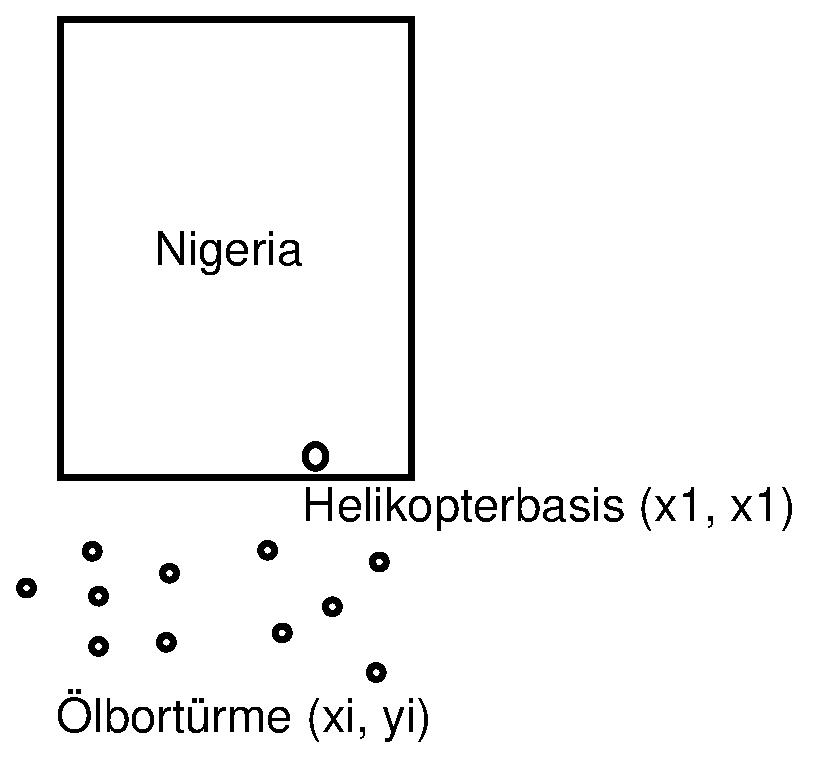
\includegraphics[width=5cm]{bilder/1-1Nigeria}

Der Helikopter fliegt eine vorgegebene Menge von Ölbohrtürmen ab um die
Pumpmenge zu regulieren und fliegt danach zurück zur Basis. Die Zeit, die
er dafür benötigt ist proportional zur Flugstrecke (euklidische Distanzen):
\[t(i,j) = \sqrt{(x_{i} - x_{j})^{2} + (y_{i} - y_{j})^{2}} = t(j,i)\]
Im Gegensatz dazu hat das Leiterplatten-Problem die $L_{\infty}$-Metrik die
auch Max Metrik genannt wird weil immer die maximale Strecke der beiden
strecken in x oder y Richtung genommen wird. Der Bohrer wird von zwei
Motoren über die Platine gefahren, die unabhängig voneinander ein und
ausgeschaltet werden können.

\subsubsection{Euklidisches Rundreise-Problem}

{\bf Gegeben:} Menge $V$ von Punkten in der euklidischen Ebene.\\
{\bf Gesucht:} Eine Tour minimaler Länge
\[n = |V| \hspace{10mm} \frac{(n-1)!}{2} \mbox{ mögliche Touren}\]

Für den Fall dass $n=23$ bräuchte ein Computer für die Auswertung einer
Tour $1\eta$s ($=10^{-9}$s) $\rightarrow$ Computer braucht zirka 178
Jahrhunderte zur Bewertung aller Touren.

\subsubsection{Plotten zusammenhängender Zeichnungen}

Das plotten eines Straßennetzes auf einer 60x60 cm Platte\\
Länge des Straßennetzes: 44,47m\\
Die Standard-Plottersoftware legte 67 km zurück und brauchte 9 Stunden und
11 Minuten.

Alternativ wurden die zu plottenden Strecken von einer "`intelligenten"'
Person durchgeführt.\\
Leerstrecke: 57,8 m\\
Zeit: 51 min

Nach Anwendung einer Matching Heuristik:
Leerstrecke: 13,62 m\\
Zeit: 36 min 45 sek.

\paragraph{Kleine Übungsaufgabe} In jedem Graphen ist die Anzahl der Punkte
mit ungerader Anzahl ein- und ausgehender Kanten gerade (Ein Satz von Euler). 

Nach Euler gilt auch, dass man einen Graphen genau dann ohne abzusetzen
und ohne eine Strecke zwei mal zu gehen zeichnen kann wenn die Anzahl der
Kanten an jedem Knoten gerade ist (einmal muss man rein, einmal raus,
falls man noch einmal rein geht, muss man auch wieder raus).

Das hilft uns nun beim Plot-Problem wir suchen nun die minimale Paarung
"`ungerader"' Knoten (die Gesamtlänge der verbindenden Kanten soll minimal
sein).

\subsubsection{Andere Rundreise-Probleme}

\paragraph{Chinesisches Postboten-Problem:} Dasselbe Problem wie beim
Plotten aber auf dünnen Graphen (Graphen mit relativ wenig Kanten).

\paragraph{Landpostboten-Problem:} Der Landpostboten muss sowohl in den
Dörfern möglichst optimal laufen als auch die Dörfer möglichst Optimal
abfahren. Das Euklidische Rundreise Problem ist hiervon ein Spezialfall
(wenn pro Dorf nur ein Haus beliefert werden muss).

\subsubsection{Euklidisches perfektes Matching-Problem}

{\bf Gegeben:} Menge $V$ von Punkten in der Euklidischen Ebene $|V|$ gerade.\\
{\bf Gesucht:} Eine Menge von Geraden Linien minimaler Gesamtlänge so dass
jeder Punkt Endpunkt genau einer Linie ist.

\section{Dualität und Schranken}

TSP-Versuch (Travelling Salesman oder eukl. Rundreise-Problem).

[Zeichnung]

Die Zeichnung stellt eine Menge von Punkten die durch Kanten verbunden sind
so dass eine Rundreise entsteht um alle Punkte herum sind nun Kreise, die
sich nicht überschneiden sondern sich falls ihre Mittelpunkte Nachbarn auf der Rundreise sind  lediglich berühren, bis auf eine
Stelle, wo eine Lücke entsteht. Jeder Kreis wird nun  genau 2 mal
durchlaufen + das eine Stück wo eine Lücke ist. Damit ist die Summe aller
Kreisdurchmesser + das extra Stück eine untere Schranke. Falls man es
schafft die Kreise so anzuordnen, dass sie sich nicht überschneiden aber
Nachbarn sich immer berühren so hat man die Optimallösung.

Oft ist aber auch keine Kombination der Kreise möglich.

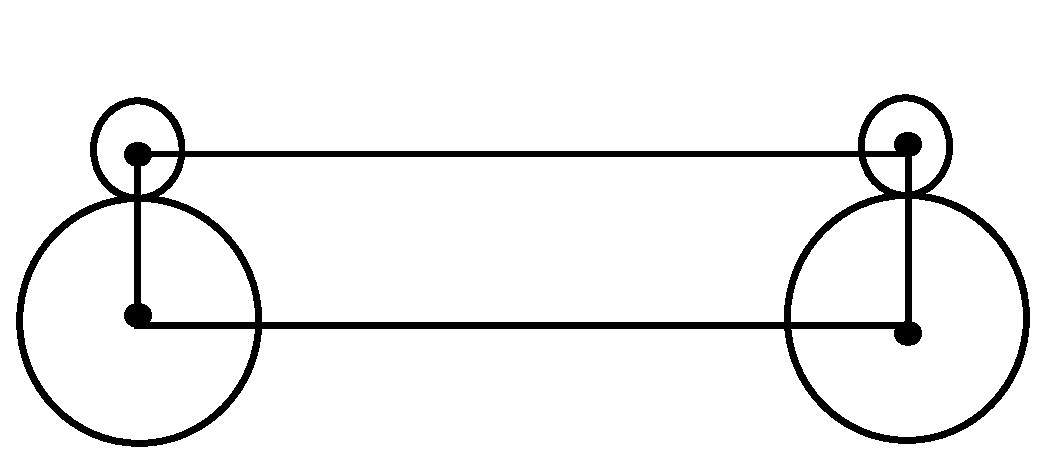
\includegraphics[width=8cm]{bilder/1-2Kreisegehtnicht}

In diesem Fall kann man dann Punkte zusammenfassen und mit "`Gräben"'


[3 Zeichnungen] habe ich leider nur ansatzweise und nicht die Zeit sie am
Computer nach zu zeichnen.

An das Euklidische Matching-Problem kann man ebenfalls mit dieser Methode
heran gehen.

\subsubsection{Euklidisches Rundreise untere Schranken Problem}

{\bf Gegeben:} Menge $V$ von Punkten in der euklidischen Ebene.\\
{\bf Gesucht:} nicht überlappendes System von Scheiben und Gräben das:
\[B=2 \sum_{v\in V} r_{v} + 2 \sum_{m\in M} w_{m}\]
maximiert.

\subsubsection{Euklidisches perf. Matching untere Schranken Problem}

{\bf Gegeben:} Menge $V$ von Punkten in der euklidischen Ebene. $|V|$
gerade.\\
{\bf Gesucht:} nicht überlappendes System von Scheiben und Gräben das:
\[\bar{B}= \sum_{v\in V} r_{v} + \sum_{m\in M} w_{m}\]
maximiert.
 
In der $L_{\infty}$-Matrix nimmt man Quadrate.

\subsection{Lineare Optimierung und untere Schranke Probleme}

\subsubsection{Euklidisches Rundreise-Problem nur mit Scheiben}

Als LP formuliert sieht es so aus:

\[\begin{array}{rcl}
(P_{1}) \hspace{7mm}  \max \displaystyle \sum_{u \in V} 2r_{u}\\
r_{u} + r_{v} &\leqq& t(u,\; v) \mbox{, für alle Paare }\{u,\; v\}\\
r_{u} &\geqq&0 \; \; \; \forall n\in V
\end{array}
\]

Das Duale LP lautet folgendermaßen:

\[\begin{array}{rcl}
(D_{1}) \hspace{7mm} \min \displaystyle \sum_{u,v} t(u,v) x_{u v}\\
\displaystyle \sum_{v\not= u} x_{u v} &\geqq & 2 \; \; \forall u \in V\\
x_{u v} &\geqq & 0 \mbox{, für alle Paare } \{u,\; v\} 
\end{array}\]

Beispiel mit vier Städten:\\\nopagebreak
\[\begin{array}{rcl}
\max \mat{rrrr}{2&2&2&2} \vect{r_{1}\\r_{2}\\r_{3}\\r_{4}}\\
s.t. \hspace {4mm} \mat{rrrr}{1&1&&\\1&&1&\\1&&&1\\&1&1&\\&1&&1\\&&1&1}
\vect{r_{1}\\r_{2}\\r_{3}\\r_{4}}
&\leqq&\vect{t(1,2)\\t(1,3)\\t(1,4)\\t(2,3)\\t(2,4)\\t(3,4)}\\
\vect{r_{1}\\r_{2}\\r_{3}\\r_{4}} &\geqq& 0
\end{array}\]

Dual

\[\begin{array}{rcl}
\min \; t(1,2)+\ldots+t(3,4) \vect{x_{12}\\\vdots\\x_{34}}\\
\mat{rrr}{x_{12}&\ldots&x_{34}}
\mat{rrrr}{1&1&&\\1&&1&\\1&&&1\\&1&1&\\&1&&1\\&&1&1} &\geqq&
\vect{2\\2\\2\\2}\\
x&\geqq& 0
\end{array}\]

\subsubsection{Hinzufügen von Gräben}

\[\begin{array}{rcl}
(P_{2}) \hspace{7mm}  \max \displaystyle \sum_{u \in V} 2r_{u}
+ \sum_{s\in M} 2 w_{s}\\
r_{u} + r_{v} + \displaystyle \sum_{s \in M, \; \left| \{u,v\} \cap s 
\right| =1} w_{s}&\leqq& t(u,\; v) \mbox{, für alle Paare }\{u,\; v\}\\
r_{u} &\geqq&0 \; \; \; \forall u\in V\\
w_{s} &\geqq& 0 \; \; \; \forall s \in M
\end{array}
\]

Das Duale LP lautet folgendermaßen:

\[\begin{array}{rcl}
(D_{2}) \hspace{7mm} \min \displaystyle \sum_{u,v} t(u,v) x_{u v}\\
\displaystyle \sum_{v\not= u} x_{u v} &\geqq & 2 \; \; \forall u \in V\\
\displaystyle \sum_{\left| \{u,v\} \cap s \right| =1} x_{u v} &\geqq& 2  \;
\; \forall s \in M\\
x_{u v} &\geqq & 0 \mbox{, für alle Paare } \{u,\; v\} 
\end{array}\]

Für jede Tour T erfüllt der Inzidenzvektor $\bar{X}$ die Restriktionen von 
$(D_{2})$.\\
$\stackrel{\mbox{\scriptsize Schwache Dualität}}{\Rightarrow}$ Die Optimallösung
für $(D_{2})$ ist eine untere Schranke für die Länge einer Tour. Wenn man
mehr Ungleichungen zu $(D_{2})$ hinzufügt erhält man eine bessere untere
Schranke ($\rightarrow$ nächstes Semester).

\paragraph{Analoge Konstruktion} für perfektes euklidisches Matching

$O$ ist die Familie der Teilmengen von $V$ ungerader Kardinalität.
\[\begin{array}{rcl}
(P_{2}) \hspace{7mm}  \max \displaystyle \sum_{u \in V} r_{u}
+ \sum_{s\in O}  w_{s}\\
r_{u} + r_{v} + \displaystyle \sum_{s \in O, \; \left| \{u,v\} \cap s
\right| =1} w_{s}&\leqq& t(u,\; v) \mbox{, für alle Paare }\{u,\; v\}\\
r_{u} &\geqq&0 \; \; \; \forall u\in V\\
w_{s} &\geqq& 0 \; \; \; \forall s \in O
\end{array}
\]

Das Duale LP lautet folgendermaßen:

\[\begin{array}{rcl}
(D_{2}) \hspace{7mm} \min \displaystyle \sum_{u,v} t(u,v) x_{u v}\\
\displaystyle \sum_{v\not= u} x_{u v} &\geqq & 1 \; \; \forall u \in V\\
\displaystyle \sum_{\left| \{u,v\} \cap s \right| =1} x_{u v} &\geqq& 1 \;
\; \forall s \in O\\
x_{u v} &\geqq & 0 \mbox{, für alle Paare } \{u,\; v\} 
\end{array}\]

Für alle $x_{u v}$ > 0 sind die entsprechenden dualen Ungleichungen mit
Gleichheit erfüllt.
Optimalität durch schwache Dualität und komplementären Schlupf.


}


\chapter{Optimale B�ume und Wege}


{
\subsubsection{Definitionen für ungerichtete Graphen}

Ungerichteter Graph $G=(V,\; E)$\\
Knotenmenge $V=V(G)$\\
Kantenmenge $E=E(G)$\\
Relation $E \rightarrow V \times V$\\
\hspace{8mm} $e=\{u,\; v\}$\\
"`e ist inzident mit $u$ und $v$ "'\\
"`$u$ und $v$ sind adjazent"'\\

\begin{tabular}{c@{\hspace{5mm}}c}
parallele Kanten&Schleife\\
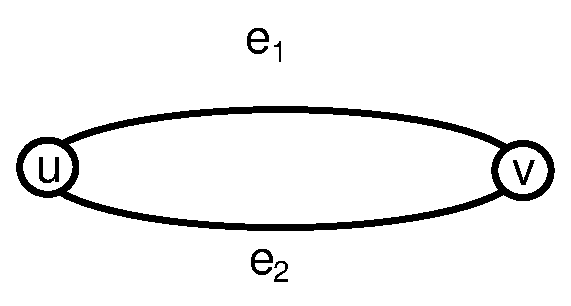
\includegraphics[width=4cm]{bilder/2-0ParalleleK}&

\includegraphics[width=1cm]{bilder/2-0Schleife}
\end{tabular}

Einfacher Graph: \begin{itemize}\item keine parallelen Kanten
\item keine Schleifen\end{itemize} 

"`$e=u v$"' \hspace{10mm} "`$e = v u$"'

Subgraph $H$ von $G$
\begin{itemize}
\item[\mbox{}] $V(H) \subseteq V(G)$
\item[\mbox{}] $E(H) \subseteq E(G)$
\end{itemize}

$A \subseteq E$ \hspace{2mm} $G\wout A$: Subgraph von $G$ nach Entfernen der Kanten in $A$ 

$B \subseteq V$ \hspace{2mm} $G \wout B$: Subgraph von G nach
entfernen der Knoten in $B$ und aller inzidenter Kanten. Kann auch als
$G(V\wout B)$ oder als durch $V \wout B $ indizierter Subgraph
bezeichnet werden. 

"`$G \wout x$"' statt $G \wout \{x\}$ für $x \in V$ oder $x \in
E$\\

$n=|V|$ \hspace{4mm} $m = |E|$ \hspace{4mm} Konvention\\

Ein Subgraph $H$ von $G$ ist aufspannend\\
$\Leftrightarrow V (H) = V$\\

Weg $P$ in $G$: Folge $\begin{array}[t]{l}
v_{0}, e_{1}, v_{1}, \ldots, e_{k}, v_{k}\\
v_{0}, v_{1}, \ldots, v_{k} \in V, \hspace{3mm} e_{1}, e_{2}, \ldots, e_{k}
\in E\\
e_{i} = v_{i-1} v_{i} \; \; \; \mbox{für}\; \;  1 \leqq i \leqq k
\end{array}$

"`Weg von $v_{0}$ nach $v_{k}$"' oder "`$(v_{0}, v_{k})$-Weg"'\\
Der Weg ist geschlossen, falls $v_{0} = v_{k}$\\
Der Weg ist einfach, falls $v_{0}, v_{1}, \ldots, v_{k}$ distinkt\\
Ein Weg ist ein Kreis falls:
\begin{enumerate}
\item Geschlossenheit
\item $v_{0}, v_{1}, \ldots, v_{k}$ distinkt sind
\item $k \geqq 1$
\end{enumerate}

$G$ hat $(u,v)$-Weg $\Rightarrow$ $G$ hat einen einfachen $(u,v)$-Weg\\
Länge von $P= v_{0}, e_{1}, v_{1}, \ldots, e_{k}, v_{k}$: $k$

$G$ ist zusammenhängend :$\Leftrightarrow$ zu jedem Knotenpaar $(u,v)$ aus $V$
gibt es einen $(u,v)$-Weg

\section{Minimal aufspanndende Bäume} 

Beispiel:


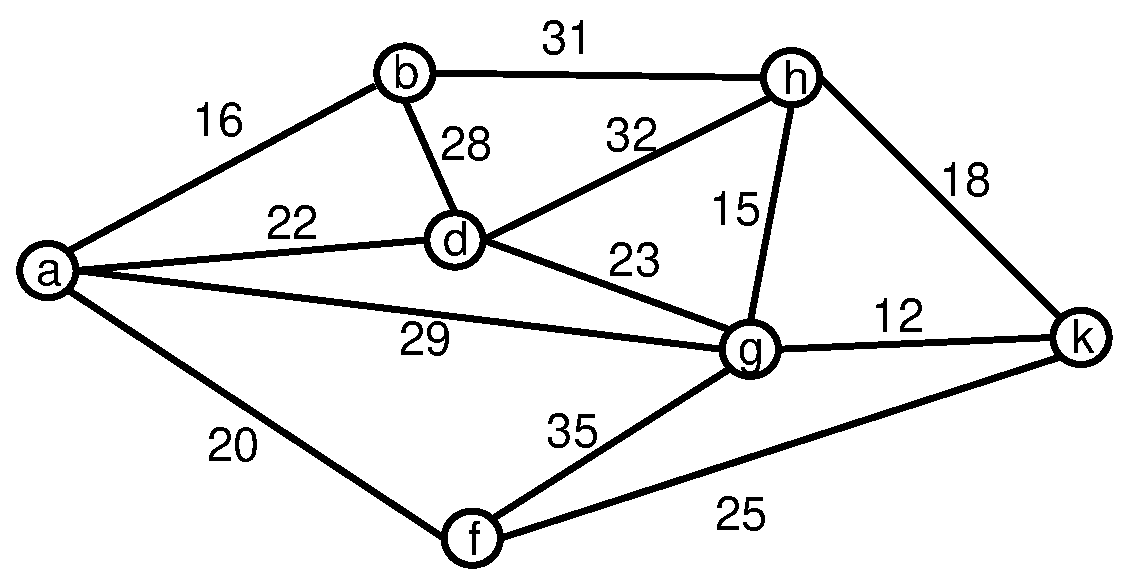
\includegraphics[width=10cm]{bilder/2-1NetzwerkP}

Dieses Netzwerk sei ein Kommunikationsnetzwerk und bilde Terminals ab und 
die den Kanten zugeordneten Zahlen entsprächen den Kosten für die direkte 
Verbindung zwischen den Terminals damit ergibt sich das

\subsubsection{Verbindungs-Problem}

Gegeben: Ein zusammenhängender Graph $G=(V,E)$ und positive Kosten für alle
$e \in E$\\
Gesucht: Ein aufspannender, zusammenhängender Subgraph mit minimalen
Kosten.

\begin{lemma}
Eine Kante $e=u v \in E$ ist Kante eines Kreises in $G$ genau dann, wenn es
einen $(u,v)$-Weg in $G \wout e$ gibt.
\end{lemma}

$\rightarrow$ die Optimallösung des Verbindungs-Problems hat keine Kreise

Einen Graphen ohne Kreis nennt man auch Wald, einen zusammenhängenden Wald
nennt man auch Baum.

\subsubsection{Minimal aufspannendes Baum-Problem}

Gegeben: Ein zusammenhängender Graph $G(V,E)$ $c_{e} \in R$ für alle $e 
\in E$\\
Gesucht: Der Aufspannende Baum in G mit minimalen Kosten (MSB) im
Englischen (MST = minimal spanning tree). Das Verbindungs-Problem und das
MSB-Problem sind äquivalent für $c_{e} > 0$.

Nun ein bisschen Wiederholung aus Informatik I:\\
Notation: $G = (V,E)$\\
$A \subseteq V$: $\delta(A) := \{u v \in E| \underbrace{u \in A,\; v\in
V \wout A}_{\mbox{\scriptsize Kanten die auf den Schnitten liegen}}\}$\\
$\delta(A)$ wird auch als "`Schnitt in G"' bezeichnet (indiziert von $A
\subseteq V$)\\ 
$\gamma(A) = \{u,v \in A, \; \; u v \in E\}$ ergibt alle Kanten in $A$

\subsubsection{Prims Algorithmus für MSB}

\begin{algorithmic}
\STATE Initialisiere $H=\left(V(H),T\right)$ als $\left\{\{r\},
\varnothing\right\}$
\WHILE{(H ist nicht aufspannender Baum)}

\STATE Füge eine Kante minimaler Kosten aus $\delta\left(V(H)\right)$ zu $H$
\ENDWHILE
\end{algorithmic}

In unserem Kommunikationsproblem erhält man nun, wenn man bei Knoten a 
anfängt:

\begin{tabular}{|c|r|}
\hline
{\bf Hinzugefügte Kante}& {\bf Kosten}\\
\hline
(a, b)& 16\\
\hline
(a, f)& 20\\
\hline
(a, d)&22\\
\hline
(d, g)&23\\
\hline
(g, k)&12\\
\hline
(g, h)&15\\
\hline
\end{tabular}

\subsubsection{Kruskals Algorithmus für MSB}

\begin{algorithmic}
\STATE Sortiere E als $<e_{1}, e_{2}, \ldots, e_{m}>$, so dass $c_{e_{1}} \leqq
c_{2} \leqq \ldots \leqq c_{e_{m}}$
\STATE Initialisiere $H=(V,T)$ als $(V, \varnothing)$
\FOR{ $i = 1$ to $m$} 
\STATE {\bf if} Endknoten von $e_{i}$ in verschiedenen Komponenten von $H$
{\bf Then} Füge
$e_{i}$ zu T hinzu.
\ENDFOR
\end{algorithmic}


mit unserem Beispiel erhält man:

\begin{tabular}{|c|r|}
\hline
{\bf Hinzugefügte Kante}& {\bf Kosten}\\
\hline
(g, k)& 12\\
\hline
(g, h)& 15\\
\hline
(a, b)&16\\
\hline
(a, f)&20\\
\hline
(a, d)&22\\
\hline
(d, f)&23\\
\hline
\end{tabular}

Beide Algorithmen können mit einer Laufzeit $O(m \log n)$ implementiert
werden.

Hier legte Prof. Jünger eine Folie auf mit Punkten um die herum ein
Analogrechner Kreise "`auf bläst"' bis zwei Kreise aneinander stoßen. Wenn
zwei Kreise aneinander stoßen und zwischen den Komponenten noch keine
Verbindung besteht so wird eine Kante dort eingefügt. Mag es jemand malen?

\subsubsection{MSB und lineare Optimierung}

Notation: Menge $\begin{array}[t]{l} A, \; p \in \RR^{A}, \; \; B \subseteq A\\
p(B) = \displaystyle \sum_{j \in B} p_{j}
\end{array}$

LPMSB $\begin{array}[t]{rcl} \min c^{T}x\\
x \left(\gamma(S)\right) &\leqq& |S| -1 \; \; \; \forall S, \varnothing \not=
S \subset V\\
x(E) &=& |V| -1\\
x_{e} &\geqq& 0 \; \; \forall e \in E
\end{array}$

In diesem Fall wird explizit nicht $x_{e} \in \{0,1\}$ gefordert, da die
Ganzzahligkeits-Bedingung das Problem sehr schwer werden lässt.

Die Inzidenzvektoren $x^{0}$ von aufspannenden Bäumen T sind zulässige
Lösungen und $c^{T}x^{0} = c(T) $, d.h. gleicher Zielfunktionswert.\\
$\Rightarrow$ der Wert von (LPMSB) ist eine untere Schranke für die Kosten
eines MSB.

\begin{satz}
Sei $x^{0}$ der Inzidenzvektor eines MSB bezüglich der Kosten $c_{e}$. Dann
ist $x^{0}$ eine Optimallösung von LPMSB.\\
Beweis: Für eine Kanten-Teilmenge $A \subseteq E$ sei $\kappa(A)$ die Anzahl
der Zusammenhangs-Komponenten des Subgraphen $(V,A)$ von $G=(V,E)$:

\[\begin{array}{rcl}
\mbox{(LPMSB')} \hspace{7mm} \min c^{T}x\\
x(A) &\leqq & |V| - \kappa(A) \; \; \forall A \subset E\\
x(E) &=& |V| -1\\
x_{e} &\geqq& 0 \; \; \forall e \in E
\end{array}\]
\end{satz}

Beweis: Das (LPMSB') hat die gleiche zulässigen Lösungen wie das (LPMSB)
d.h. auch die gleiche Optimallösung. In $x(A) \leqq |V| - \kappa (A)$
setzen wir speziell $A = \gamma(S)$ und erhalten:

\[\begin{array}{rcl}
x\left(\gamma(S)\right) &\leqq & |V| - \underbrace{\kappa\left(\gamma(S)
\right)}_{\geqq | V \wout S| + 1}\\
&\leqq& |V|-| V \wout S | -1\\
&=& | S | -1
\end{array}\]

Umgekehrt folgt $x(A) \leqq |V| - \kappa(A)$, denn:\\
Sei $A \subseteq E $ und $s_{1}, s_{2}, \ldots, s_{k} \; \left(k = \kappa(A)
\right)$ die Knotenmengen der Zusammenhangs-Komponenten von $(V,A)$.\\
Dann gilt $\begin{array}[t]{rcl} 
x(A) &\leqq & \displaystyle \sum_{i=1}^{k} x\left(\gamma (s_{i})\right)\\
&\leqq & \displaystyle \sum_{i=1}^{k} (|s_{i}| -1)\\
&=& |V|-k
\end{array}$

Es reicht also zu zeigen $x^{0}$ ist optimal für (LPMSB'). Wir zeigen dies
nun für ein $x^{0}$ das Ergebnis aus Kruskals Algorithmus ist. Im (LPMSB')
können wir für die Zielfunktion auch schreiben $\-max -c^{T}x$. Damit
erhalten wir als duales LP:
\[
\begin{array}{rcl}
\mbox{(DLPMSB')} \hspace{7mm} \min \displaystyle \sum_{A \subset E \mbox{\scriptsize so 
dass } e \in A} (|V| - \kappa(A)) y_{A}\\
 \displaystyle \sum_{A \subset E \mbox{ \scriptsize so dass }
e \in A} y_{A} &\geqq& -c_{e} \; \; \forall e \in E\\
y_{A} &\geqq& 0 \; \; \forall A \subset E
\end{array}
\]
$y_{E}$ ist in diesem Fall nicht vorzeichen-beschränkt. Mittels Kruskals
Algorithmus konstruieren wir nun eine Optimallösung von (DLPMSB').

Sei $e_{1}, e_{2}, \ldots, e_{m}$ die sortierte Folge der Kanten in
Kruskals Algorithmus.
\[ R_{i} := \{ e_{1}, e_{2}, \ldots, e_{i}\} \hspace{3mm} (1 \leqq i \leqq
m) \hspace{3mm} R_{0} := \varnothing \]
Weiterhin definieren wir $y^{0}$:
\[\begin{array}{rcl}
y^{0}_{R_{i}} &=& c_{e_{i+1}} - c_{e_{i}}\\
y^{0}_{R_{m}} &=& -c_{e_{m}} \hspace{3mm} \\ \hspace{3mm} y_{A}^{0} = 0 
\mbox{ sonst } \hspace{3mm} (A \not=R_{i})
\end{array}\]
Es gilt nun (wg. Sortierung) $y_{A}^{0} \geqq 0 \hspace{3mm} \forall
A \not= E$ und mit $e=e_{i}$:
\[\begin{array}{rcl}
\displaystyle \sum_{A \subset E \mbox{\scriptsize  so 
dass } e \in A} y^{0}_{A} &=& \displaystyle \sum^{m}_{j=1} y^{0}_{R_{j}} =
\sum^{m-1}_{j=i} (c_{e_{j+1}} - c_{e_{j}}) - c_{e_{m}}\\
&=& c_{e_{i+1}} - c_{e_{i}} + c_{e_{i+2}} -  c_{e_{i+1}} + \ldots
+  c_{e_{m}} -  c_{e_{m-1}} - c_{e_{m}}\\
&=& -c_{e_ {i}} = - c_{e} \end{array}
\]

$\Rightarrow$ alle "`$\geqq$"' sind mit "`="' erfüllt.\\
$\Rightarrow \left\{ \begin{array}{l}y^{0} \mbox{ ist zulässig für
(DLPMSB')}\\
\mbox{kompl. Schlupf $x_{e}^{0} > 0 \Rightarrow \displaystyle \sum_{A
\subset E \mbox{ so dass } e \in A} y_{A} = -c_{e} \; \; \forall e \in E$}
\end{array}\right.$

Noch zu zeigen:
\[\mbox{Kompl. Schlupf: } y_{A}^{0} > 0 \Rightarrow x^{0}(A) = | V | -
\kappa(A)\]
Sei $y_{A} > 0 \Rightarrow A = R_{i}$ für $1\leqq i \leqq m$\\
Annahme: $x^{0} (R_{i}) < |V| - \kappa(R_{i})$\\
$x^{0} (R_{0}) = |V| - \kappa(R_{0})$ 
$\Rightarrow \exists e \in R_{i}$: Hinzufügen von $e$ zu $T \cap R_{i}$
erniedrigt die Zahl der Zusammenhangs-Komponenten von $(V,R_{i} \cap T)$\\
$\Rightarrow e \not \in T \hspace{3mm} \lightning$ denn Kruskal hätte $e$
gewählt, d.h. $e \in T$

Damit ergibt sich nun insgesamt: $x^{0},\;y^{0}$ sind zulässig und erfüllen
die komplementären Schlupfbedingungen.\\
$\Rightarrow x^{0}$ ist optimal für (LPMSB')\\
$\Rightarrow x^{0}$ ist optimal für (LPMSB)

Bemerkung: Dies beweist die Korrektheit von Kruskals Algorithmus.

\section{Kürzeste Wege}
Anwendung: Kürzeste Fahrstrecke von A nach B in einem Straßen-Netzwerk.\\
Es gibt auch Einbahnstraßen $\rightarrow$ gerichtete Graphen\\
Gerichteter Graph $G=(V,E)$ auch genannt "`Digraph"' mit \\
$V=V(G)$ Knoten \\
$E(G)$ gerichtete Kanten oder auch Bögen (arc)\\
\begin{tabular}{ll}
Für $e \in E$:& $t(e)$: Ende von $e$ (tail)\\
&$h(e)$: Spitze von $e$ (head)
\end{tabular}
 
Die anderen Begriffe gelten analog zu nicht gerichteten Graphen.\\
Den zu einem gerichteten Graphen zugeordneten ungerichteten Graphen erhält
man durch das weglassen der Richtung.\\
Parallele Kanten sind Kanten die dieselbe Spitze und und die gleichen
Enden haben. Antiparrallele Kanten sind zwei Kanten bei denen die eine dort
die Spitze hat wo die andere das Ende und umgekehrt.

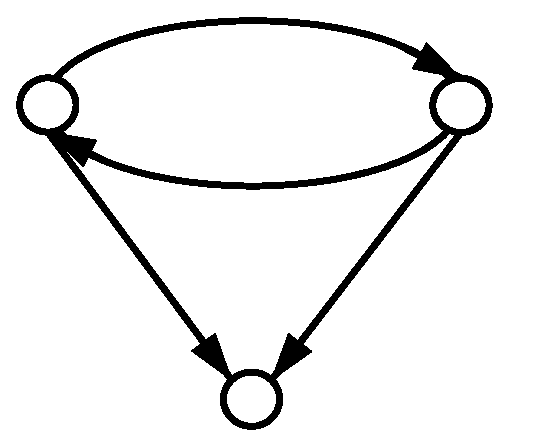
\includegraphics[height=3cm]{bilder/2-2einfachnichte} 

Als Digraph ist dieser Graph ein einfacher Graph als ungerichteter Graph
nicht.

$e=u v \rightarrow t(e)=u$, $h(e) = v$

Kanten $e_{i}$ eines Weges $P= v_{0}, e_{1}, v_{1}, e_{2}, \ldots e_{k},
v_{k}$. Der Weg heißt vorwärts gerichtet falls $t(e_{i})=v_{i-1}$ und
$h(e_{i})=v_{i}$. Analog ist ein gerichteter Kreis ein Kreis bei dem alle
Kanten vorwärts gerichtet sind.

\subsubsection{Kürzeste Wege Problem}
Gegeben: Digraph $G$, Knoten $v$ aus $V$, Gewichte $c_{e} \in \RR \; \forall 
e \in E$ 

Gesucht: Für alle $v \in V$ einen gerichteten Weg von $r$ nach $v$ mit
minimalen Kosten, falls ein solcher existiert.

Konvention: Zur Vermeidung der Nicht-Existenz eines $(r,v)$-Weges fügt man
Kanten $r v \in E$ mit sehr hohem Gewicht hinzu.

Ohne Beschränkung der Allgemeinheit kann von einem einfachen Graphen
ausgegangen werden, da man alle parallelen Kanten auf die günstigste Kante
reduziert.

Die Grundidee der folgenden Algorithmen sieht dabei folgendermaßen aus:
\begin{itemize}
\item $\forall v  \in V$ gerichteter Weg von $r$ nach $v$ mit Kosten 
$y_{v}$
\item Finde eine Kante $v w \in E$ mit $y_{v} + c_{v w} < y_{w}$: dann existiert ein
kürzester Weg (in Bezug auf alle Wege die wir bisher kennen) von $v$ nach
$w$ mit Kosten $y_{v} + c_{v w}$. 
\item Sind die $y_{v}\;\; (v \in V)$ Kosten für kürzeste $(u,v)$-Wege so 
gilt:\\ ($\ast$) $y_{v} + c_{v w} \geqq y_{w}$\\
$y \in R^{v}$ heißt zul. Potential falls  ($\ast$) gilt und $y_{r}=0$
Falls $y_{r} \not= 0$, einfach $y_{v}$ durch $y_{v} - y_{r}$ ersetzen.  
\end{itemize}

\begin{lemma} \label{Potential}
Sei $y$ ein zulässiges Potential und $P$ ein $(r,v)$-Weg (gerichtet), dann
gilt: $c(P) \geqq y_{v}$\\
\end{lemma}

Beweis: Sei $P= v_{0}, e_{1}, v_{1}, e_{2}, \ldots e_{k}, v_{k}$, mit $v_{0} 
= r$, $v_{k}=v$ so gilt:
\[c(P) = \sum^{k}_{i=1} c_{e_{i}} \geqq \sum^{k}_{i=1}(y_{v_{i}} -
y_{v_{i-1}}) = y_{v_{k}} - \underbrace{y_{v_{0}}}_{=0} = y_{v_{k}} 
\hspace{3mm} \mbox{q.e.d}\]

\begin{lemma}
Es existiert eine Lösung des Kürzeste Wege Problems, die nur Kanten eines
aufspannenden Baumes enthält
\end{lemma}

Beweis: Subwege von kürzesten Wegen sind kürzeste Wege\\
$\Rightarrow \forall v \in V, \; \; v \not=r$ genügt die letzte Kante
eines gerichteten $(r,v)$-Weges

\subsubsection{Fords Algorithmus}

\begin{algorithmic}
\STATE Initialisiere:\\
$y_{r} := 0, \; \; y_{v} := \infty \; \; \forall v \not= r$\\
$p_{r} := 0, \; \; p_{v} := -1 \; \; \forall v \not= r\; \; \; (0,-1) \not
\in V$
\WHILE{($y$ kein zul. Potential)}
\STATE Finde eine Kante $v w$ mit $y_{v} + c_{v w} < y_{w}$
\STATE setze $y_{w} := y_{v} + c_{v w}$ und $p_{w} := v$
\ENDWHILE
\end{algorithmic}

\subsubsection{Beispiel 1}

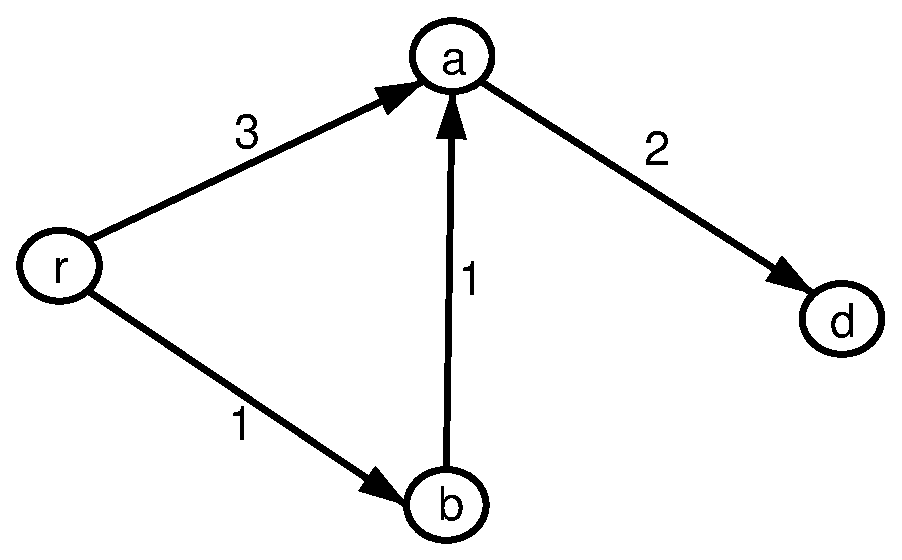
\includegraphics[width=6cm]{bilder/2-2FordBsp1}

\begin{tabular}{l|r|r|r|r|r|r|r|r|r|r|}
&\multicolumn{2}{|c|}{Start}&\multicolumn{2}{|c|}{$v w=r a$}&
\multicolumn{2}{|c|}{$v w=r b$}&\multicolumn{2}{|c|}{$v w=ad$}&
\multicolumn{2}{|c|}{$v w=a b$}\\ \hline
&y&p&\hspace{2mm}$\;$y&p&\hspace{2mm}$\;$y&p&\hspace{2mm}$\;$y&p&
\hspace{2mm}$\;$y&p\\ \hline
r&0&0&&&&&&&&\\
a&$\infty$&-1&3&$r$&&&&&2&$b$\\ 
b&$\infty$&-1&&&1&$r$&&&&\\
d&$\infty$&-1&&&&&5&$a$&4&$a$
\end{tabular}

Eigenschaften
\begin{enumerate}
\item Nach jeder Iteration gilt:
\[y_{v} \geqq y_{p(v)} + c_{p(v)v}\]
Dies gilt mit "`="' wenn $y_{v}$ und $p(v)$ gesetzt werden, nachher kann
$y_{p(v)}$ nur kleiner werden.
\item Nach Terminierung gilt:
\[y_{v} \geqq y_{p(v)} + c_{p(v)v}\]
\end{enumerate}

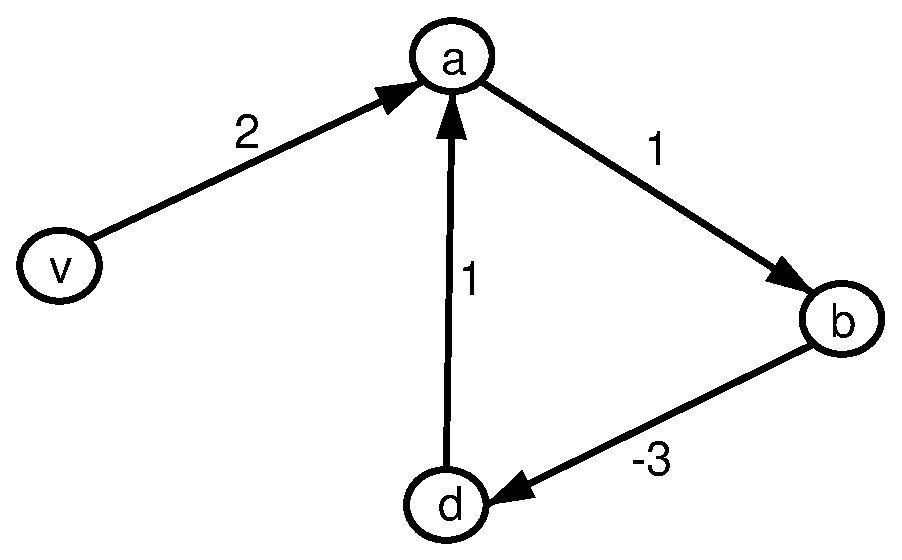
\includegraphics[width=6cm]{bilder/2-2FordBsp2}

\begin{tabular}[c]{l|r|r|r|r|r|r|r|r|r|r|r|r}
&\multicolumn{2}{|c|}{Start}&\multicolumn{2}{|c|}{$v w=r a$}&
\multicolumn{2}{|c|}{$v w=ab$}&\multicolumn{2}{|c|}{$v w=b d$}&
\multicolumn{2}{|c|}{$v w=da$}&\multicolumn{2}{|c}{$v w=ab$}\\ \hline
&y&p&\hspace{2mm}$\;$y&p&\hspace{2mm}$\;$y&p&\hspace{2mm}$\;$y&p&
\hspace{2mm}$\;$y&p&\hspace{2mm}$\;$y&p\\ \hline
r&0&0&&&&&&&&&&\\
a&$\infty$&-1&2&$r$&&&&&1&$d$&&\\
b&$\infty$&-1&&&3&$a$&&&&&2&$a$\\
d&$\infty$&-1&&&&&0&$b$&&&&
\end{tabular} $\ldots$

Hier terminiert das Verfahren nicht, da $y_{a}, \; y_{b}, \; y_{c}, \;
\rightarrow - \infty$.\\
Grund: negativer Kreis $a b d$.

Der Algorithmus soll dies erkennen. Es gibt aber auch Anwendungen für
negative Kreise, z.B. im Währungstausch.

\begin{tabular}{c}
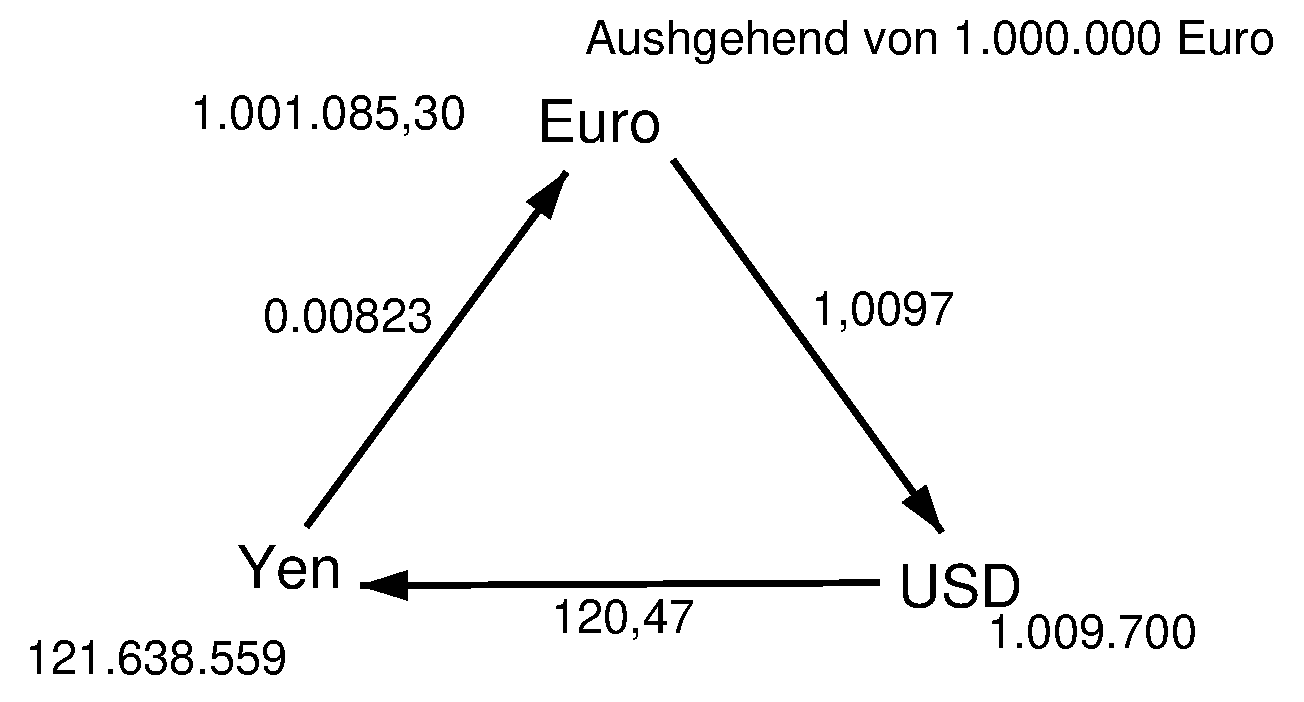
\includegraphics[width=8cm]{bilder/2-2Arbitrage}\\
Arbitrage-Möglichkeiten mit den Kursen vom 18.11.2002
\end{tabular}

Gesucht sind also Folgen $v_{0}, v_{1}, \ldots, v_{k} = v_{0}$ mit:
\[\prod^{k}_{i=1} r_{v_{i-1} v_{i}} > 1\] 

Kosten: $c_{u v} = -\log r_{u v}$

Gewinn falls $\sum_{i=1}^{k} \log r_{v-1v_{i}} = - \log \prod_{i=1}^{k}
r_{v_{i-1}v_{i}} < 0$

\begin{lemma} \label{Ford1}
Hat $(G,c)$ keinen negativen Kreis, so gilt nach jeder Iteration von Fords
Algorithmus:
\begin{enumerate}
\item Ist $y_{v} \not= \infty$ so ist $y_{v}$ Kosten eines einfachen 
$(r,v)$-Weges 
\item Ist $p(v) \not = -1$ so definiert $p$ einen einfachen $(r,v)$-Weg mit
Kosten höchstens $y_{v}$ 
\end{enumerate}
\end{lemma}

Beweis: 
\begin{enumerate}
\item Sei $y_{v}^{j}$ der Wert $y_{v}$ nach $j$ Iterationen.\\
$y_{v}^{j}\not= \infty \rightarrow  y_{v}^{j}$ Kosten eines
$(r,v)$-Weges $P$.\\
Annahme: $P$ ist nicht einfach $\Rightarrow \exists$ Folge $v_{0}, v_{1},
\ldots, v_{k}$,  $v_{k}= v_{0}$\\
Iterationszahlen $q_{0} < q_{1} < \ldots < q_{k}$ mit $y_{v-1}^{q_{i-1}} +
c_{v_{i-1}v_{i}} = y_{v_{i}}^{q_{i}}$\\
und Kosten des geschlossenen Weges:
\[\begin{array}{rcl}
\displaystyle \sum_{i=1}^{k} c_{v_{i-1}v_{i}} &=& \displaystyle \sum_{i=1}^{k} 
(y_{v_{i}}^{q_{i}} - y_{v_{i-1}}^{q_{i-1}})\\
&=& y_{v_{k}}^{q_{k}} - y_{v_{0}}^{q_{0}} < 0
\end{array}\]
$y_{v_{k}}$ wurde in Iteration $q_{k}$ erniedrigt. Also haben wir einen
negativen Kreis und damit Widerspruch. 
\item Annahme $P$ ist nicht einfach\\
$\Rightarrow \exists v_{0}, v_{1}, \ldots , v_{k}$, $v_{k}= v_{0}$\\
$p(v_{i})=v_{i-1}$  \hspace{3mm} $(1\leqq i \leqq k)$\\
Die Kosten des geschlossenen Weges sind $\leqq 0$, da $c_{p(v)v}  \leqq
y_{v} - y_{p(v)}$\\
Die letzte Änderung ergibt: $p(v)$ mit Verkleinerung von $y_{p}(v_{i})$
$\Rightarrow$ "`$<$"'\\
$\Rightarrow$ negativer Kreis, Widerspruch  
\end{enumerate}

Die Kosten sind höchstens $y_{v}$:
Es gebe einen einfachen $(r,v)$-Weg und sei $v_{0}, e_{1}, v_{1}, \ldots,
e_{k}, v_{k}$ mit $v_{0} = r$, $v_{k}=v$, $p(v_{i}) = v_{i-1}, \; \; \; 
(1 \leqq i \leqq k)$\\
Kosten $\displaystyle \sum_{i=1}^{k} c_{v_{i-1}v_{i}} \leqq  \sum_{i=1}^{k}
(y_{v_{i}} - y_{v_{i-1}}) = y_{v} - y_{r} = y_{v}$ q.e.d.

\begin{satz}
Hat $(G,c)$ keinen negativen Kreis, so terminiert Fords Algorithmus nach
endlich vielen Schritten mit einem korrekten Ergebnis
\end{satz}

Beweis:\\
$\exists$ nur endlich viele einfache gerichtete Wege in $G$.\\
Lemma \ref{Ford1} $\Rightarrow$ Es gibt nur endlich viele mögliche Werte
für die $y_{v}$. In jedem Schritt wird ein $y_{v}$ erniedrigt und keines
erhöht $\rightarrow$ endlich viele Schritte.

Bei Terminierung definiert $p$ einfache $(r,v)$-gerichtete Wege für alle
$v \in V$ mit Kosten höchstens $y_{v}$.\\
Lemma \ref{Potential} $\Rightarrow$ Es gibt keine kürzere
$(r,v)$-gerichtete Wege.

\begin{satz} \label{Potential2}
$(G,c)$ hat ein zulässiges Potential genau dann, wenn es keinen negativen
Kreis gibt.
\end{satz}

Beweis:\\
"`$\Rightarrow$"' negativer Kreis $\Rightarrow$ kein zulässiges Potential

"`$\Leftarrow$"' $(G,c)$ habe keinen negativen Kreis:\\
Man konstruiere folgenden Graphen $(G',c')$:

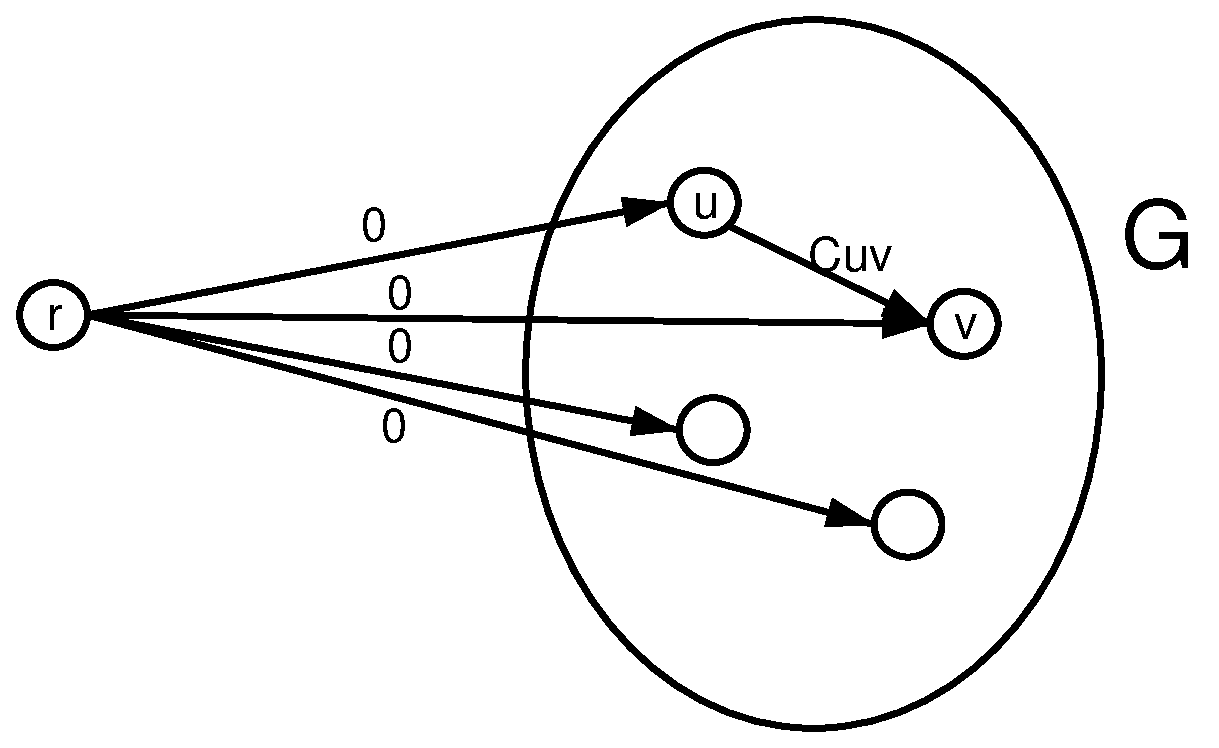
\includegraphics[width=9cm]{bilder/2-2NegatKreis}

$r$ ist jeweils mit allen Knoten von $G$ durch gerichtete Kanten des
Gewichtes 0 verbunden. Damit hat $(G',c')$ keinen negativen Kreis.
Anwendung von Fords Algorithmus auf $(G',c')$ gibt zulässiges Potential für 
$(G',c')$. Diese ist auch zulässiges Potential für $(G,c)$. q.e.d.

Satz \ref{Potential2} Gilt auch ohne Annahme der Existenz von
$(r,v)$-Wegen.\\
Problem: nicht einfache beliebig kurze $(r,v)$-gerichtete Wege.\\
Die Suche nach einfachen (r,v)-Wegen (endlich viele!) ist jedoch
NP-schwierig.

\begin{satz}
Falls $c_{e} \in \ZZ$ für alle $e \in E$:
\[ c = 2 \max_{e \in E} | c_{e} | + 1 \]
und $(G,c)$  hat keinen negativen Kreis so terminiert Fords Algorithmus
nach höchstens $c n^{2}$ Iterationen
\end{satz}
Beweis: Übungsaufgabe

\subsection{Zulässige Potentiale und lineare Optimierung}

\begin{satz} 

Sei $G$ ein gerichteter Graph, $r,s \in V$, $c \in \RR^{E}$\\
Falls für alle $v \in V$ ein kürzester  $(r,v)$-Weg existiert, so gilt:\\
\[\begin{array}{cl}
&\min \left\{c(P) | P \mbox{ ist $(r,s)$ gerichteter Weg} \right\}\\
=& \max \left\{ y_{s} | y \mbox{ ist ein zulässiges Potential}\right\}
\end{array}\]
\end{satz}
Beweis: Analyse von Fords Algorithmus

Als duales LP formuliert erhält man (ohne Bedingung $y_{r}=0$):
\[\begin{array}{rcl}
\mbox{(DLPKW)} \hspace{7mm} \max y_{s} -y_{r}\\
y_{w} - y_{v} \leqq c_{v w} \; \; \; \forall v,w \in E
\end{array}\]

Für das LP definieren wir:\\
Sei $b_{v} = \left\{ \begin{array}{l} 1 \mbox{ falls } v =s\\
-1 \mbox{ falls } r =v\\
0 \mbox{ sonst}\\
\end{array} \right.$

\[\begin{array}{rcl}
\mbox{(LPKW)} \hspace{7mm} \min \displaystyle \sum_{e \in E} c_{e} x_{e}\\
\displaystyle \sum_{w \in V, \; \; v w \in E} x_{w v} -  \sum_{w \in V, \;
\; w v \in E} x_{v w} &=& b_{v} \; \; \; \forall v \in V\\
x_{v w} &\geqq & 0  \; \; \; \forall v w \in E
\end{array}\]

Jedem $(r,s)$-gerichteten Weg $P$ entspricht eine zulässige Lösung für
(LPKW) mit Wert $c(P)$.
$x_{e}^{P} = $ Anzahl des Vorkommens von $e$ in $P$. ($\in \{0,1\}$ falls
$P$ einfach ist).

\subsubsection{Verhalten des Simplexalgorithmus beim LPKW}

Gegeben sei folgender Graph:

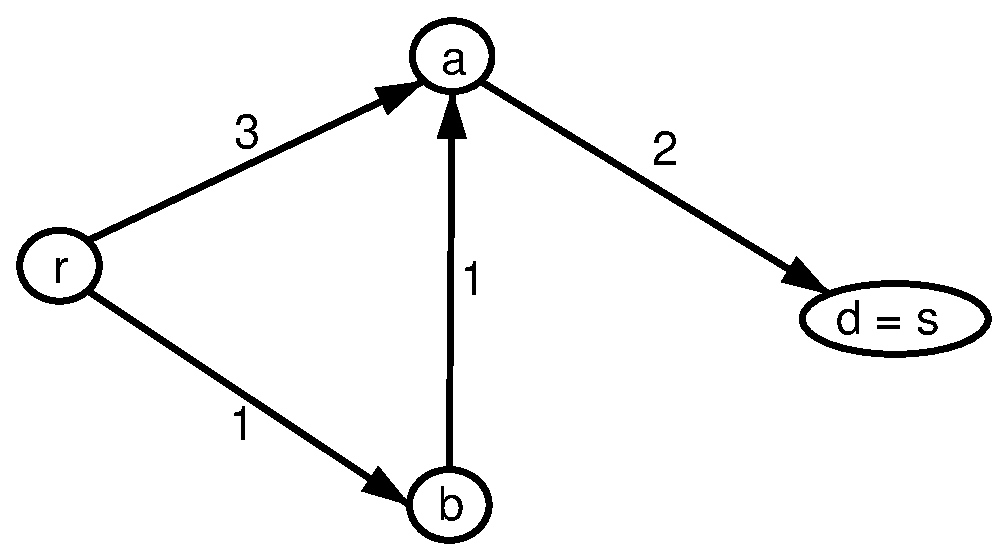
\includegraphics[width=6cm]{bilder/2-2SimplLPKW}

Dann ergibt sich folgender Aufbau:

A \hspace{3mm}
\begin{tabular}{c|rrrr|}
\multicolumn{1}{c}{\mbox}&r a&r b& b a&\multicolumn{1}{r}{ad}\\ \cline{2-5}
r&-1&-1&&\\
a&1&&1&-1\\
b&&1&-1&\\
d&&&&1\\
\cline{2-5}
\end{tabular} $=$ \begin{tabular}{|r|}
\multicolumn{1}{c}{b}\\\hline-1\\\mbox{}\\\mbox{}\\1\\\hline
\end{tabular}
\hspace{4mm}$\begin{array}{rcl}
\mbox{(LKWP)} \hspace{3mm} \min c^{T}x\\
A x &=& b\\
x &\geqq& 0
\end{array}$

c\hspace{12mm}\begin{tabular}{|rrrr|}
\hline 3&1&1&2\\ \hline
\end{tabular}

Der Simplexalgorithmus betrachtet nun eine Folge von Basislösungen wobei
eine Basis einer "`max. linear unabh. Kantenteilmenge"' entspricht. Es ist
also eine "`Spaltenbasis"' von A.

In jeder Iteration hat man eine Basis $B$ und $x,y$ mit $x_{e} = 0 \; \; \forall
e \not\in B$.
\[y_{w} - y_{v} = c_{v w} \forall v w \in B\]

\begin{satz} \label{Spaltenb-Baum}
Sei $G$ ein zusammenhängender gerichteter Graph, $A$ die Knoten-Kanten
Inzidenzmatrix.

$A_{\cdot J}, \; \; J \subseteq E$ ist eine Spaltenbasis von $A$ genau dann
wenn $J$ die Kantenmenge eines Aufspannenden Baumes in $G$ ist.
\end{satz}

Beweis: Übungsaufgabe

Baum $T_{1}$

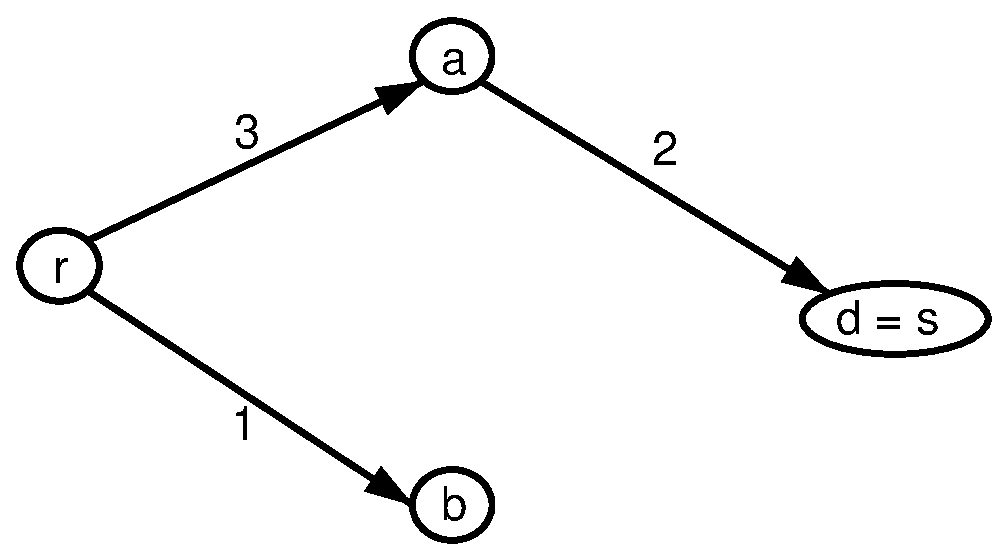
\includegraphics[width=6cm]{bilder/2-2SimplLPKW2}

Ein Basiswechsel Beispiel.

B \hspace{3mm}
\begin{tabular}{c|rrr|}
\multicolumn{1}{c}{\mbox}&r a&r b&\multicolumn{1}{r}{ad}\\ \cline{2-4}
r&-1&-1&\\
a&1&&-1\\
b&&1&\\
d&&&1\\
\cline{2-4}
\end{tabular} $=$ \begin{tabular}{|r|}
\multicolumn{1}{c}{y}\\\hline0\\3\\1\\5\\\hline
\end{tabular}

c\hspace{12mm}\begin{tabular}{|rrr|}
\hline 3&1&2\\ \hline
\end{tabular}

reduzierte Kosten: $c_{b a} - y^{T}A_{\cdot b a} = 1 -2 = -1 < 0$

$\rightarrow$ $b a$ geht in die Basis, $r a$ raus (hat die Spitze am selben
Punkt).

Baum $T_{2}$

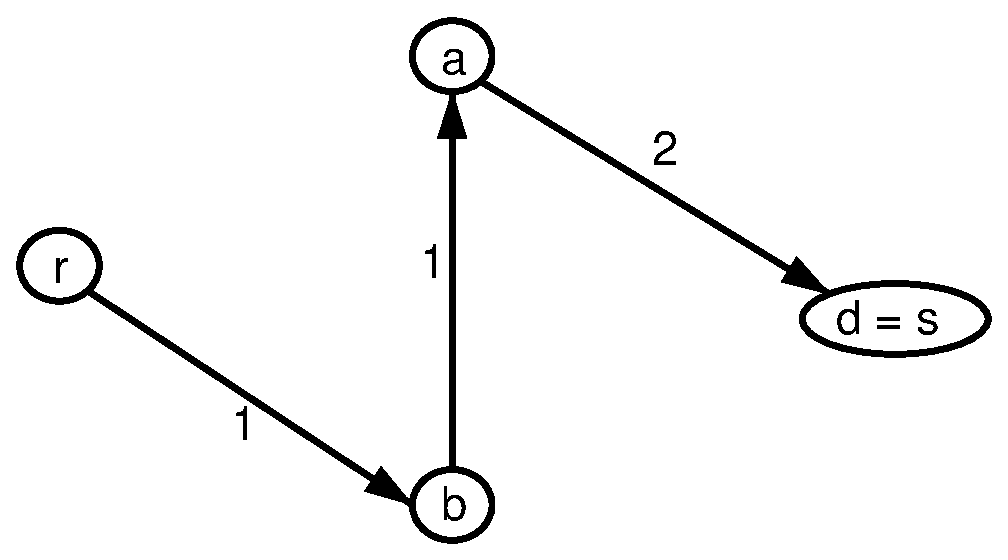
\includegraphics[width=6cm]{bilder/2-2SimplLPKW3}

B \hspace{3mm}
\begin{tabular}{c|rrr|}
\multicolumn{1}{c}{\mbox}&r a&b a&\multicolumn{1}{r}{ad}\\ \cline{2-4}
r&-1&&\\
a&&1&-1\\
b&1&-1&\\
d&&&1\\
\cline{2-4}
\end{tabular} $=$ \begin{tabular}{|r|}
\multicolumn{1}{c}{y}\\\hline0\\2\\1\\4\\\hline
\end{tabular}

c\hspace{12mm}\begin{tabular}{|rrr|}
\hline 3&1&2\\ \hline
\end{tabular}

reduzierte Kosten: $3-2 = 1 > 0$

Die Gleichungen $y_{w} - y_{v} = c_{v w} \forall v w \in B$ gelten in Fords
Algorithmus nicht immer, d.h. jede Iteration dieses speziellen Simplex
Verfahrens entspricht einer Folge von Iterationen in Fords Algorithmus
(Änderung des Baumes gefolgt von $y$-Änderungen bei gleichem Baum. 

\subsection{Varianten des Ford Algorithmus}

Korrekturschritte in konstanter Zeit. Laufzeit abhängig von der
Reihenfolge  $S= <f_{1}, f_{2}, \ldots, f_{e}>$ der gewählten Kanten. Bei
schlechter Wahl erhält man eine Laufzeit von $\Theta(2^{|E|})$ (Übungen)

Ein $(r,v)$-Weg $P= \; \; r=v_{0}, e_{1}, v_{1}, \ldots, c_{k}, v_{k} = v$
ist in $S$ eingebettet falls $e_{1}, e_{2},\ldots_{k}$ eine geordnete
Subsequenz von $S$ ist.

\begin{lemma} \label{Ford2}
Wenn Fords Algorithmus die Sequenz $S$ benutzt, so gilt für jedes $v \in V$
und jeden $(r,v)$-Weg der in $S$ eingebettet ist $y_{v} \leqq c(P)$
\end{lemma}

Beweis: Sei $P = \; \;  \underbrace{v_{0}}_{\mbox{\scriptsize$=r$}}, 
e_{1}, v_{1}, \ldots, c_{k}, \underbrace {v_{k}}_{\mbox{\scriptsize $= v$}}$\\
Nach erster Iteration mit $e_{1}: y_{v_{1}} \leqq y_{r} + c_{e_{1}}$\\
Nach zweiter Iteration mit $e_{2}: y_{v_{2}} \leqq y_{v_{1}} + c_{e_{1}}+ 
c_{e_{2}}$\\
Nach dritter Iteration mit$\begin{array}[t]{rcl}e_{k}: y_{v} = y_{v_{k}} &\leqq & y_{v_{k-1}} + c_{e_{k}}\\
&\leqq & \displaystyle \sum_{i=1}^{k} c_{e_{i}} = c(P). \hspace{3mm}
\mbox{q.e.d}\end{array}$

Also suchen wir $S$ mit kürzesten eingebetteten $(r,v)$-Wegen für alle $v
\in V$ $S$
"`kurz"' da die Laufzeit proportional zur Länge.

\subsubsection{Ford-Bellmann-Algorithmus}

Jeder einfache gerichtete Weg in $G$ ist eingebettet in
$<s_{1},s_{2},s_{3},
\ldots, s_{n-1} >$ mit $s_{i} =$ irgendeine Permutation von $E= \{ e_{1},
e_{2}, \ldots, e_{m}\}$

\begin{algorithmic}
\STATE Initialisiere $y, \; p$;
\STATE $i=0$;
\WHILE{($i < n$ und $y$ kein zulässiges Potential)}
\STATE i := i+1;
\FOR{ $e=e_{1}$ to $e_{m}$}
\STATE $v=t(e)$; $w=h(e)$;
\IF{$(y_{v} + c_{v w} < y_{w})$}
\STATE $y_{w} := y_{v} + c_{v w}$; $p_{w} := v$
\ENDIF
\ENDFOR
\ENDWHILE
\IF{$(i < n)$} 
\STATE "`Kürzester Weg gefunden"'
\ELSE 
\STATE STOP "`es existiert ein negativer Kreis"'
\ENDIF
\end{algorithmic}


\begin{satz}
Der Ford-Bellmann Algorithmus ist korrekt und hat Laufzeit $O(n m)$.
\end{satz}

Beweis: Korrektheit wg. Lemma \ref{Ford2}, Laufzeit offensichtlich.

Verbesserungen der Laufzeit sind nur bei speziellen Annahmen über $G$ und
$c$ möglich. Vorgestellt werden nun Verbesserungen in der Praxis:

\paragraph{Vorwärts-Stern-Datenstruktur}
\mbox{} 

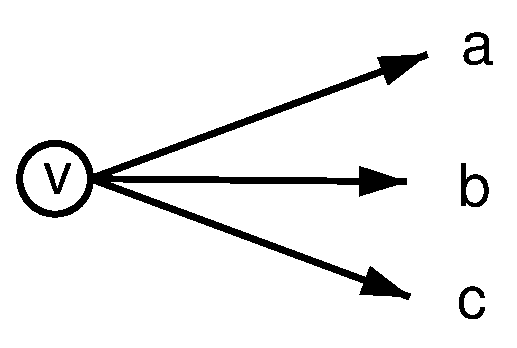
\includegraphics[width=4cm]{bilder/2-2VorwaertsStern} $L(v)=<a,b,c>$

Weiterhin benötigen wir:\\
$Q= <f_{1}, f_{2}, \ldots, f_{e}>$ Schlange (Queue) von Kunden.\\
$v \Leftarrow Q$ ergibt $v=q_{1},\; \;  Q = <f_{2}, f_{3}, \ldots,
f_{e}>$\\
$Q \Leftarrow v$ ergibt $Q= <f_{1}, f_{2}, \ldots, f_{e}, v>$\\
Zusätzlich Inzidenzvektor: isinQ Q[v]\\
Anzahl der Knoten in Q: numQ 

dies erlaubt delete, append $Q \stackrel{?}{=} \varnothing, \; \; v \stackrel{?}{\in} Q$ in konst.
Zeit (keine Negativen Kreise).

\begin{algorithmic}
\STATE Initialisiere $y,\;p$;
\STATE $Q:= <v>$;
\WHILE{$(Q \not= \varnothing)$}
\STATE $v \Leftarrow Q$;\\
\FORALL{$\left(w \in L(v)\right)$}
\IF{$(y_{v} + c_{v w} < y_{w})$}
\STATE $y_{w} := y_{v} + c_{v w}$; $p_{w} := v$ \}\\
\IF{$(w \not\in Q)$}
\STATE $Q \Leftarrow w$;
\ENDIF
\ENDIF
\ENDFOR
\ENDWHILE
\end{algorithmic}

\paragraph{Azyklische Graphen}
\mbox{}\\
Keine gerichteten Kreise, insbesondere keine negativen Kreise. Kompatible
Knoten Sequenz $<v_{1}, v_{2}, \ldots, v_{n}>$ für alle Knoten $v_{i},
v_{j} \in E$ gilt: $i < j$ kann in Zeit $O(m)$ gefunden werden (Topologische
Sortierung, siehe Übungsaufgabe 20).

OBdA: sei $r=v_{1}$
\[ r=v_{i} \; \Rightarrow \; v_{j} \; \; \; (j < i) \mbox{ nicht erreichbar} \]
wie oben, aber:

\begin{algorithmic}
\STATE $\vdots$
\FOR{$i=1$ to $n$}
\FORALL{$\left(w \in L(v_{i})\right)$}
\STATE (jeder Pfad ist eingebettet)
\IF{$(y_{v} + c_{v w} < y_{w})$}
\STATE $y_{w} := y_{v} + c_{v w}$; $p_{w} := v$ 
\ENDIF
\ENDFOR
\ENDFOR
\end{algorithmic}

\begin{satz}
In azyklischen Graphen kann das kürzeste Wege Problem in Zeit $O(m)$
gelöst werden
\end{satz}

Nicht negative Kosten:
\[ c_{e} \geqq 0 \; \; \forall e \in E\]
Wie vorhin, aber Knotensequenz dynamisch bestimmt nach $v_{1}, v_{2},
\ldots, v_{i}$.\\
Wähle $v_{i+1} = v \in \{v_{1}, v_{2}, \ldots,v_{i}\}$ mit minimalem
$y_{v}$.

\begin{lemma} \label{UvorV}
Für alle $w \in V$ sei $y'_{w}$ der Wert von $y_{w}$ wenn $w$ gewählt wird.
Wird $u$ vor $v$ gewählt. So gilt $y'_{u} \leqq y'_{v}$.
\end{lemma}

Beweis: Annahme $y'_{v} < y'_{u}$ und $v$ ist der erste Knoten bei dem das
passiert.\\
Als $u$ gewählt wurde galt: $y'_{u} = y_{u} \leqq y_{v}$. Nach Wahl von $u$
und vor Wahl von $v$ wurde $y_{v} < y'_{u}$, sagen wir das letzte Mal
bei Wahl von $w$
\[v_{1}, v_{2}, \ldots, u, \ldots, w, \ldots,v,\ldots\]
Also fand bei $w$ die letzte Erniedrigung von $y_{v}$ statt. Zu diesem
Zeitpunkt wurde gesetzt:
\[y_{v} := y'_{w} + c_{w v}\]
Aber $\left. \begin{array}{rcl}
y'_{w} &>& y'_{u} \hspace{3mm} \mbox{(erster Fehler bei $v$)}\\
c_{v w} &\geqq& 0
\end{array}
\right\} y'_{v} \geqq y'_{u} \hspace{4mm} \lightning$

\subsubsection{Dijkstras Algorithmus}

\begin{algorithmic}
\STATE Initialisiere $y$, $p$;
\STATE $S := V$
\WHILE{$(S \not= \varnothing)$}
\STATE wähle $v \in S$ mit $y_{v}$ minimal
\STATE entferne $v$ aus $S$;
\STATE Bearbeite Vorwärtsstern von $v$ (aber nur Kanten mit $vw$ mit $w \in
S$!)
\ENDWHILE
\end{algorithmic}


\begin{satz}
Falls $c_{e} \geqq 0 \; \; \forall e \in E$, so ist Dijkstras Algorithmus
korrekt und läuft in $O(n^{2})$
\end{satz}

Beweis:\\
Am Ende gilt ($\ast$) $y_{v} + c_{v w} \geqq y_{w} \; \; \forall \; v w \in
E$

Annahme: ($\ast$) gilt nicht\\
($\ast$) galt nach Bearbeitung von Knoten v $\Rightarrow y_{v}$ wurde
später erniedrigt, etwa als $q$ bearbeitet wurde. \\
$\Rightarrow y_{v} = \underbrace{y'_{q}}_{\geqq y'_{v}} + \underbrace{c_{q v}}_{\geqq 0}  \geqq y'_{v}$ 
also nicht erniedrigt $\lightning$\\
denn wenn q nach v bearbeitet wurde $\stackrel{\mbox{\scriptsize Lemma
\ref{UvorV}}}{\Rightarrow} y'_{q} \geqq y'_{v}$\\
$w \not \in S$: $y_{v} \geqq y_{w} \stackrel{\mbox{\scriptsize Lemma
\ref{UvorV}}}{\Rightarrow} y_{v} + \underbrace{c_{v w}}_{\geqq 0} \geqq
y_{w v}$ also hier kein Test nötig. 

Laufzeit $O(m)$ für Vorwärtsstern plus die Zeit zum Finden von $v$ mit
minimalem $y_{v}$. Naiv implementiert erhält man damit eine Laufzeit von
$O(n^{2})$

Aus der Informatik I. Für Dünne Graphen mit Heaps $O(m \log n)$. Noch besser
geht es mit Fibonacci Heaps (Wer hat die Fibonacci Beweise nicht geliebt?):
$O(n \log n + m)$.

Wie dem auch sei, sei $S(n,m)$ die Zeit, die benötigt wird.

Beobachtung:\\
Kennt man ein zulässiges Potential $y$ so kann man den Kostenvektor $c$
nach $c' \geqq 0$ transformieren: $c'_{v w} = c_{v w} + y_{v} - y_{w} (\geqq 0)$ 
denn  $\forall (r,s)$-Wege $P$: sind die Kosten: 
\[c'(P) = c(P) + y_{r} - y_{s}\]  
Anwendung: Kürzeste $(r,v)$-Wege für alle Paare (r,v). Allgemein beste
Methode: n mal wie gehabt.\\
Zeit $O(n \cdot S(n,m))$, wenn $c \geqq 0$, also $O(n^{2}m)$ im allgemeinen
Fall.

Verbesserung von $O(n^{2}m)$: Wenn Ford Bellman einmal ausgeführt ist
liefert er uns ein zulässiges Potential für jeden Punkt.
\[\left. \begin{array}{l}
\mbox{Transformation s.o.}\\
\mbox{$(n-1)$ mal Dijkstra}\end{array} \right\} \mbox{zusammen } O(n \cdot
S(n,m))
\]

\subsubsection{Einheitskosten und Breitensuche}

Finde $(r,v)$-Wege mit minimaler Kantenzahl.

\begin{lemma} \label{ErsterW}
Falls $c_{e} = 1$ für alle $e \in E$, so ist der erste endliche Wert für
$y_{v}$ auch der endgültige. Wird $y_{v}$ vor $y_{w}$ zugewiesen, so gilt
$y_{v} \leqq y_{w}$.
\end{lemma}

Beweis: klar für $v=r$. Sei $v \not=r$ und $v$ später gewählt als Knoten
$u \Rightarrow y_{v} \geqq y_{u}$ (Lemma \ref{UvorV}).\\
zu endgültig: Erster endliche Wert für $y_{v}$ wird gesetzt zu $y_{w+1}$
[Knoten $w$ wird vor $v$ gewählt]


Behauptung $y_{v}$ wird nicht mehr geändert \\
Annahme: bei  Wahl eines anderen Knotens z.B. $q$ wird $y_{v}$ erniedrigt
zu $y'_{v}$.\\
Situation: $\ldots w \ldots v \ldots q$\\
$q$ wird nach $w$ gewählt $ \Rightarrow y_{q} \geqq y_{w}$\\
$y'_{v} = y_{q} + 1 \geqq y_{w} + 1 = y_{v} \; \; \; \lightning$ zu
erniedrigt.

\begin{satz}
Bei Einheitskosten kann Dijkstras Algorithmus mit Laufzeit $O(m)$
implementiert werden.
\end{satz}
Beweis: Wegen Lemma \ref{ErsterW} kann man den nächsten Knoten aus einer
Schlange wählen ($y_{w}$ sind überflüssig).

Dieser Algorithmus heißt auch Breitensuche.

\begin{algorithmic}
\STATE Initialisiere p;
\STATE $Q = <r>;$\\
\WHILE{$(Q \not= \varnothing)$}
\STATE $v \Leftarrow Q$;
\FORALL{$(w \in L(v))$}
\IF{$(p(w) = -1)$}
\STATE $Q \Leftarrow w$;
\STATE $p(w) = v$;
\ENDIF
\ENDFOR
\ENDWHILE
\end{algorithmic}



}

\chapter{Maximale Flussprobleme}

{
\section{Flüsse und Schnitte}

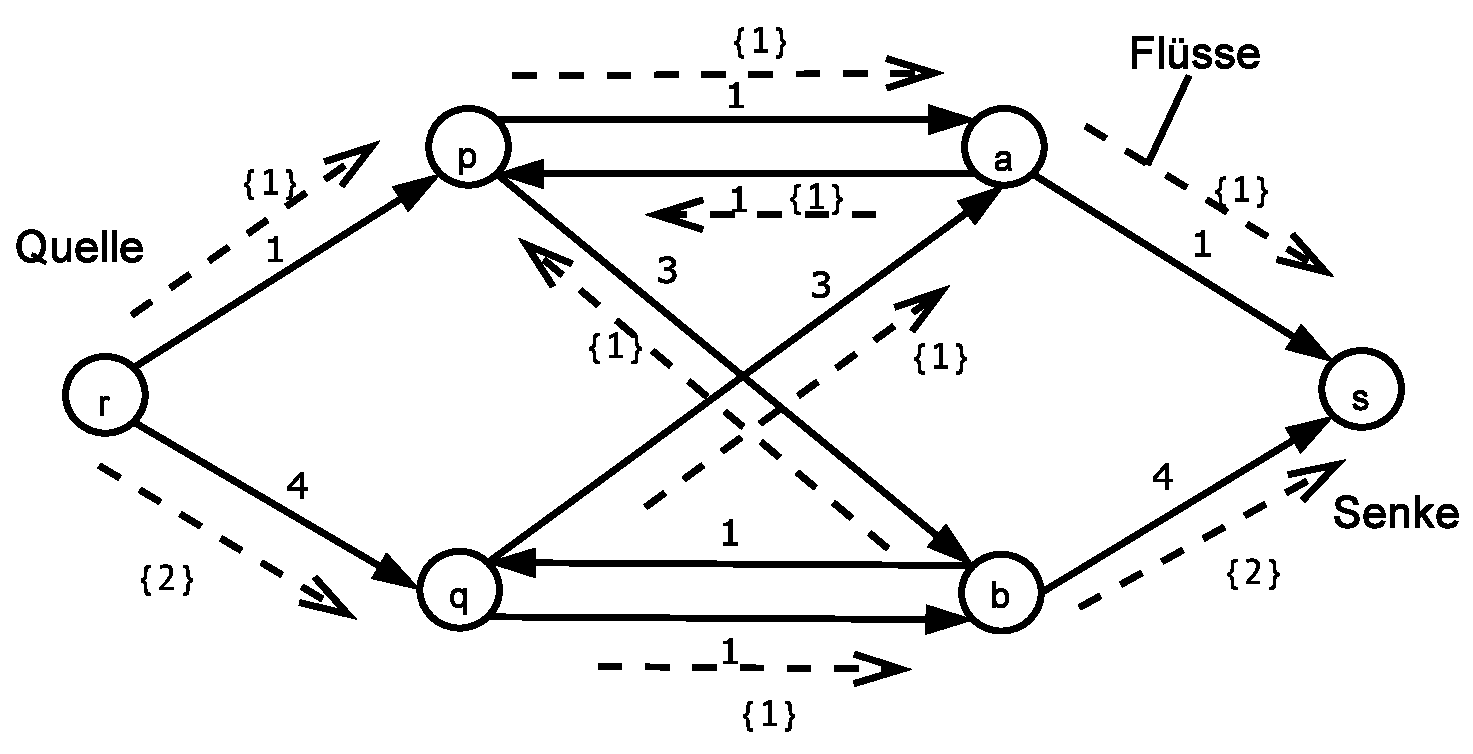
\includegraphics[height=4cm]{bilder/3-0Maxfluss}

Die Flüsse können nun als Kollektion von einfachen $(r,s)$-Wegen (die nicht
notwendigerweise verschieden sind) betrachtet werden. In der Grafik sind
allerdings nur die kumulierten Flüsse dargestellt. $\{ p_{1}, p_{2}, \ldots
p_{k} \}$ mit:
\begin{enumerate}
\item jedes $e \in E$ ist höchstens $u_{e}$
\item die Anzahl der Wege werden maximiert
\[ x_{e} = | \{ i | P_{i} \mbox{ benutzt } e\} |\]
\end{enumerate}
Bedingungen für $x$:\\
\[ (\ast) \hspace{3mm} \sum_{w \in V, \; w v \in E} x_{w v} - \sum_{w\in V,
\; v w \in E} x_{v w} = 0\]
\[(\ast \ast) \hspace{3mm} 0 \leqq x_{v w} \leqq u_{v w} \forall \; v w \in E\]
$x_{v w}$ ist ganzzahlig $\forall v w \in E$. Die Zielfunktion lautet:
\[ max \sum_{w \in V,\;  w s \in E} x_{w s} - \sum _{w \in V,\;   s w \in E}
x_{s w} = k \mbox{ ( $=$ Flusswert})\]

Damit haben wir das Maximum ganzzahlige Flussproblem formuliert.

$x \in R^{E}$ heißt Fluss, falls $x$ $(\ast)$ erfüllt.\\
$x \in R^{E}$ heißt zulässiger Fluss, falls $x$ $(\ast \ast)$ erfüllt.

$f_{x} (v) := \displaystyle \sum_{w \in V, \; w v \in E} x_{w v} -  \sum_{w \in V, \; v w
\in E} x_{v  w}$ Dies nennt man auch "`Nettofluss"' oder "`Überschuss"' bei
$v$

$(\ast)  = f_{x}(v) = 0 $ ist die "`Flusserhaltungsbedingung"' und $f_{s}$
ist der Flusswert.

\begin{lemma} \label{Familie}
Eine Familie $\{P_{1}, P_{2},\ldots, P_{k}\}$ von $(r,s)$-Wegen mit $|\{i |
P_{i} \mbox{ benutzt }e\}| \leqq u_{e}$ existiert genau dann wenn ein
ganzzahliger zulässiger $(r,s)$-Fluss mit Flusswert $k$ existiert.
\end{lemma}

Beweis: $\exists$ Familie von Wegen $\Rightarrow \exists$ ein Fluss,
klar.\\
"`$\Leftarrow$"' Gegeben sein ein Fluss $x \in R^{e}$ mit Flusswert $k$.
Entferne Kreise:
\[ x_{e} := x_{e} -1 \; \; \forall \; e \in \mbox{ Kreis } C\]
$\Rightarrow$ Flusswert $k$ bleibt.

Finde $P_{1}$ : $v \ldots s$ (mit alle n Kanten $> 0$) $x_{e} := x_{e} -1
\forall \; e \in P_{1}$. $\rightarrow$ Flusswert ist $k-1$.

Finde $P_{k}$

\paragraph{Maximales Flussproblem} \mbox{}\\
\[\begin{array}{rcl}
\max f_{x}(s)\\
f_{x}(v) &=&0 \; \; \forall v \in V \wout \{r,s\}\\
0 \leqq x_{e} &\leqq& u_{e} \; \; \forall\; e \in E
\end{array}\]

Für einen Kreisfluss der Menge $\alpha$ gilt: $0 < \alpha \leqq \min
\{u_{e}, e \in C\}$

\begin{lemma}
Jeder zulässige $(r,s)$-Fluss ist die Summe von höchstens $m$ Kreis und
Weg-Flüssen.
\end{lemma}

Beweis: Analog zu \ref{Familie} mit Kreis und Wegeflüssen.

\subsubsection{Maximale Flüsse und minimale Schnitte}

Definition des gerichteten Schnittes $R$:
\[ R \subseteq V, \; \; \delta(R) = \{v w | v w \in E, \; v \in R, \; w \not\in
R\}\]
Ein $(r,s)$-gerichteter Schnitt: $r \in R, \; s \not\in R$\\
$A \subseteq V, \; \bar{A} := V \wout A \hspace{3mm} \delta(v)$ für
$\delta(\{v\})$, $\delta(\bar{v})$ für $\delta(\bar{\{v\}})$.

\begin{lemma}\label{SchnittFluss}
Für jeden $(r,s)$-Schnitt $\delta(R)$ und jeden $(r,s)$-Fluss $x$ gilt
$x(\delta(R))$ - $x(\delta(\bar{R})) = f_{x}(s)$
\end{lemma}

Im Beispiel: $R=\{r,q,p\} \Rightarrow 4-1 = 3$

Beweis: 
\[\begin{array}{rcl}
\displaystyle \sum_{v \in \bar{R} \wout \{s\}} f_{x}(v) &=&0\\
f_{x} (s) &=& f_{x}(s)\\
\mbox{addiert: } \hspace{3mm} \displaystyle \sum_{v \in \bar{R}} f_{x}(v)
&=& f_{x}(s) 
\end{array}\]

Wenn Kante $e$ beide Endpunkte in $R$ hat:
\[\begin{array}{rcl}
e = v w, \; v,w \in R&:& \mbox{tritt nicht auf, 0-Koeffizient in Summe}\\
v, w \in \bar{R}&:& \begin{array}[t]{l}
\left. \begin{array}{l} 
\mbox{$v$-Gleichung, Koeffizient -1}\\
\mbox{$w$-Gleichung, Koeffizient 1}
\end{array}
\right\} \mbox{Koeffizient 0} \end{array}\\
v \in R, \; w \not\in  R&:& \mbox{Koeffizient 1}\\
v \not\in R, \; w \in R&:& \mbox{Koeffizient -1}
\end{array}
\]
$f_{x}(v) = \displaystyle \sum_{w v \in E} x_{w v} - \sum_{v w \in E}
x_{v w}$\\
$\Rightarrow \displaystyle \sum_{v \in R} f_{x}(v) = x(\delta(R)) - x (\delta(\bar{R}))
\hspace{3mm} \mbox{q.e.d.}$

\begin{korollar}\label{FlussSchnittKap}
Für jeden zulässigen $(r,s)$-Fluss $x$ und jeden $(r,s)$-Schnitt
$\delta(R)$ gilt:
\[f_{x}(s) \leqq u (\delta(R)) \hspace{7mm} \mbox{$u = $ Kapazität}\]
\end{korollar}
Im Beispiel: $ R = \{r,p,q\} \rightarrow f_{x}(s)\leqq 8$

Beweis: $\begin{array}[t]{rcl}
x(\delta(R)) &\leqq & u (\delta(R))\\
-x (\delta(\bar{R})) &\leqq &0\\
\stackrel{\ref{SchnittFluss}}{\Rightarrow} f_{x}(s) &\leqq & u (\delta(R))
\hspace{3mm} \mbox{q.e.d.}
\end{array}$\\
Dies ist ähnlich zur schwachen Dualität.


\begin{satz}\label{MaxFlowMinCut}
Max Flow Min Cut Theorem\\
Gibt es einen maximalen $(r,s)$-Fluss, so gilt
\[\max\{f_{x}(s) | x \mbox{ ist zul. $(r,s)$-Fluss}\} = 
\min \{u(\delta(R))| \delta (R) \mbox{ ist ein $(r,s)$-Schnitt}\}\]
\end{satz}
(entspricht der starken Dualität)

Beweisidee:
\begin{enumerate}
\item Finde $(r,s)$-Weg $P$ mit $x_{e} < u_{e} \forall \; e \in P$
\item Erhöhe Fluss (alle $x_{e} \in P$) um $\min\{u_{e} - x_{e} | e \in
P\}$
\end{enumerate}
Im Beispiel: kein maximaler Fluss, trotzdem funktioniert diese Idee nicht.

Generalisierung: $\forall$ Vorwärtskanten $x_{e} < u_{e}$ und $\forall$
Rückwärtskanten $x_{e} > 0$ 

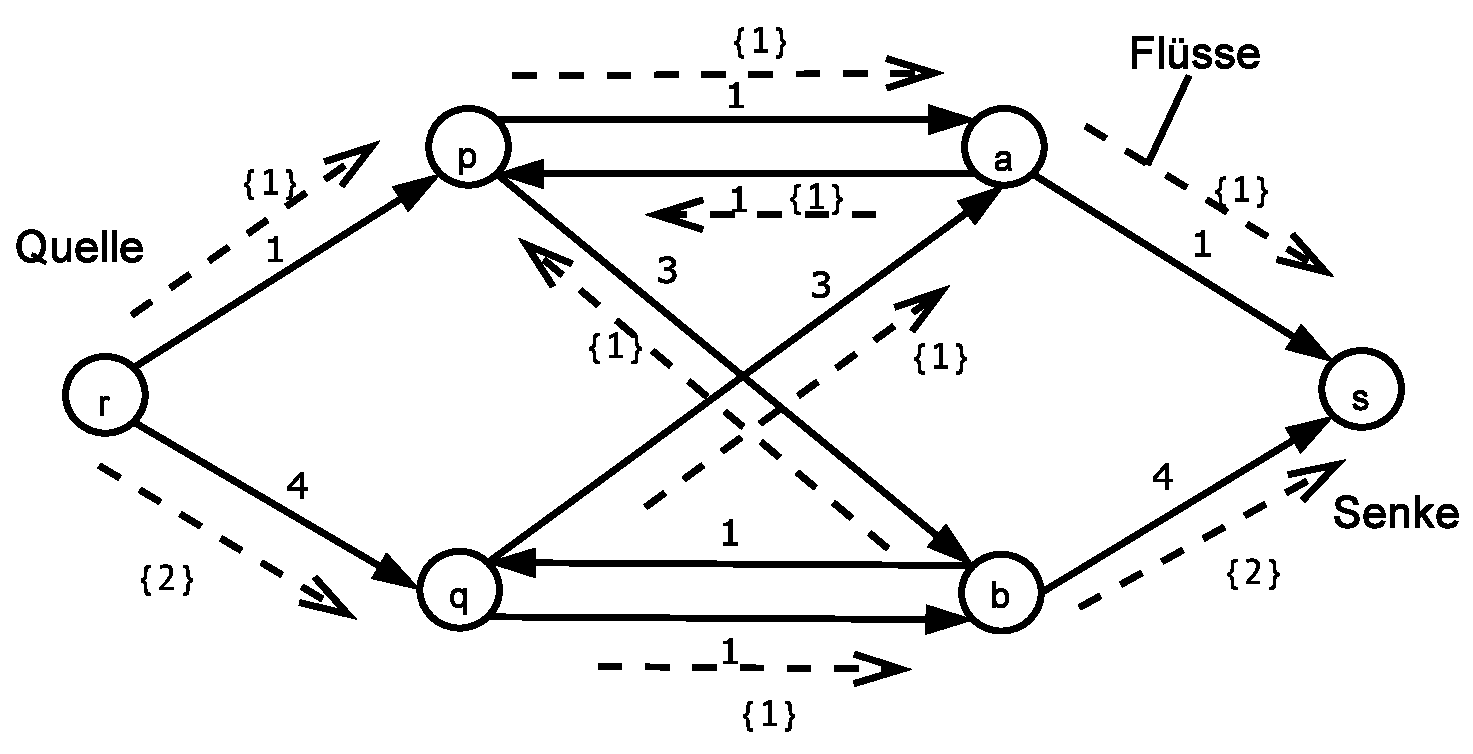
\includegraphics[height=4cm]{bilder/3-0Maxfluss}

Man betrachte den Weg $r,q,a,p,b,s$ und setze Kante $p,a$ zu 0.\\
$\rightarrow$ $p,b$ kann auf 2 gesetzt werden, $b,s$ auf 3, $r,q$ auf 3 und
$q,a$ auf 2.\\
Nun $R=\{r,q,a\}=4$, also ist 4 der optimale Fluss. (Der Schnitt $R$ muss
immer die Quelle enthalten).

Beweis: Mit Korollar \ref{FlussSchnittKap} ist zu zeigen:
\[\exists \mbox{ zul. Fluss x, } \exists \mbox{ Schnitt } \delta(R): \; \;
f_{x} = u (\delta(R))\]
Sei $x$ maximal zulässiger Fluss\\
Def: $R:= \{ v \in V| \exists \mbox{ $x$ erhöhender $(r,v)$-Weg} \}
\hspace{3mm}$ "`$(u\{r\})$"'

Behauptung: $\delta(R)$ ist zugehöriger optimaler Schnitt.\\
Es gilt: $r \in R$, $s \not\in R$ ($x$ optimal)\\
$\forall\;v w \in \delta(R) \; \; \; x_{v w} = u_{v w}$ (sonst
$r\rightarrow\ldots\rightarrow v \rightarrow w$, $x$ erhöhend, aber $w \not\in
R$)\\
$\forall \; v w \in  \delta(\bar{R}) \; \; \; x_{v w} = 0$ (analog).
$\stackrel{\ref{SchnittFluss}}{\Rightarrow} f_{x}(s) = \underbrace{ x
(\delta(R))}_{= u(\delta(R))} -  \underbrace{x (\delta (\bar{R}))}_{=0} =
u(\delta(R))$

\begin{satz}
Ein zulässiger Fluss ist maximal genau dann, wenn kein $x$-erhöhender Weg
existiert.
\end{satz}
Beweis: \\
"`$\Rightarrow$"' klar\\
"`$\Leftarrow$"' Beweis von Satz \ref{MaxFlowMinCut} liefert Schnitt
$\delta(R)$ mit $f_{x}(s) = u (\delta(R)) \stackrel{\ref{FlussSchnittKap}}{
\Rightarrow} x$ ist maximaler zulässiger Fluss. q.e.d.

\begin{satz}
Ist $u$ ganzzahlig und existiert ein maximal zulässiger Fluss, so existiert
ein ganzzahliger maximal zulässiger Fluss.
\end{satz}
Beweis: wähle ganzzahligen maximalen Fluss. $x$ und $u$ ganzzahlig.
$\exists$ x-erhöhender Weg $\Rightarrow \exists$ höherer ganzzahliger Fluss.\\
Einfacher: Existiert ein maximaler zulässiger Fluss so existiert auch der
minimal zulässige Schnitt. Der wiederum setzt sich als Summe der
ganzzahligen Kapazitäten zusammen $\Rightarrow$. Diese Summe ist dann auch 
ganzzahlig.

\begin{korollar}
Ist $x$ ein zulässiger $(r,s)$-Fluss und $\delta(R)$ ein
$(r,s)$-Schnitt, so ist $f_{x}(s)$ Maximum und $u(\delta(R))$ Minimum genau
dann wenn: 
$x_{e} = u_{e} \; \; \forall e \in \delta(R)$\\
$x_{e} = 0 \;\; \forall e \in \delta(\bar{R}) \mbox{ q.e.d.}$
\end{korollar}

\section{Erhöhender Weg (Augmenting Path) Algorithmus}

\begin{algorithmic}
\STATE Starte mit zulässigem Fluss $x$ (z.B. $x=0$)
\WHILE{($\exists x$-erhöhender Weg $P$)}
\STATE $E_{1} := \min \{ u_{e} - x_{e} | e \mbox{ ist Vorwärtskante in
}P\}$
\STATE $E_{2} := \min \{x_{e} | e \mbox{ ist Rückwärtskante in } P \}$
\STATE $E := \min \{E_{1}, E_{2} \}$ \hspace{3mm} "`$x$-Breite von $P$"'
\IF{$(E = \infty)$}
\STATE STOP \hspace{3mm} "`kein maximaler Fluss"'
\ELSE 
\STATE erhöhe Fluss auf $P$ um $E$
\ENDIF
\ENDWHILE
\STATE STOP $x$ maximaler Fluss
$R:= \{v \in V | \exists \mbox{$x$-erhöhender $(r,v)$-Weg} \}$ min Schnitt
$\delta(R)$.
\end{algorithmic}

\subsubsection{Suche nach einem $x$-erhöhendem Weg}
Hilfsdigraph $G(x)$: $V(G(x)) := V$\\
$v w \in E(G(x))$ genau dann wenn $v w \in E$ und $x_{v w} < u_{v w}$ oder $w v 
\in E$ und $x_{w v} > 0$.\\
$(r,s)$-Wege in $G(x) \Leftrightarrow x$-erhöhende Wege in $G$\\
Genannt Breitensuche: Zeit $O(m)$ pro Iteration. Im Beispiel 
(Hilfsdigraph zum ersten Fluss mit Flusswert 3):


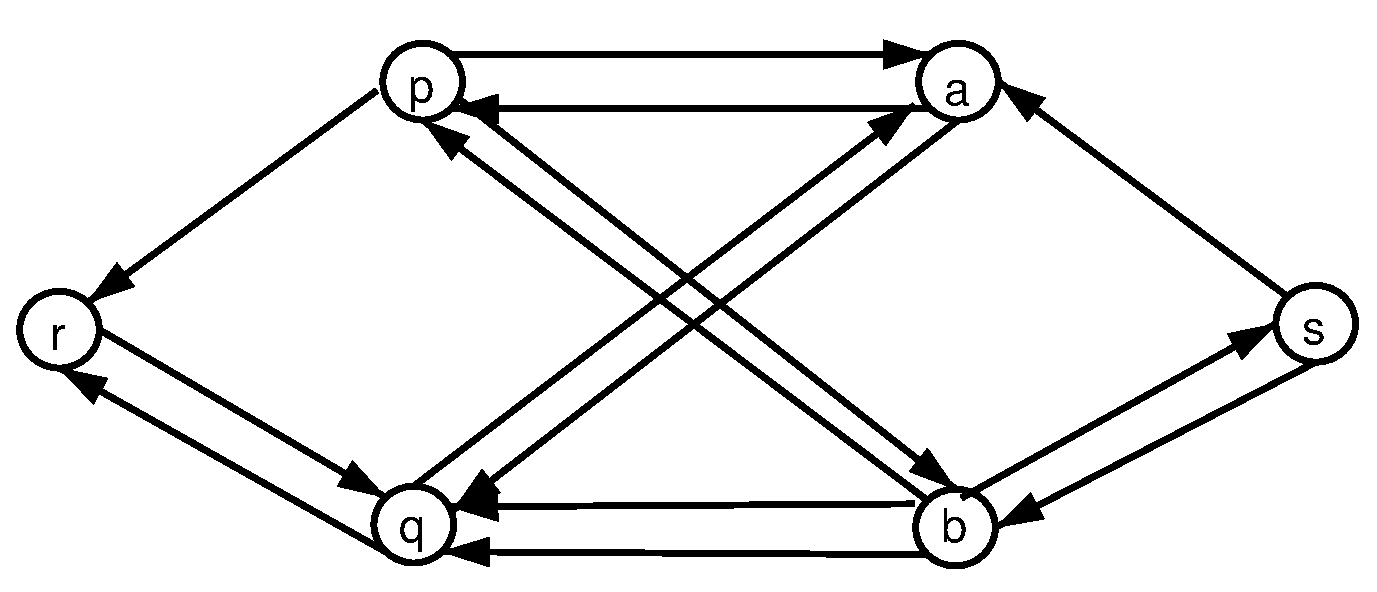
\includegraphics[height=3cm]{bilder/3-0MaxflussDig}

\begin{satz} \label{EW}
Ist $u$ ganzzahlig und der maximale Flusswert $k < \infty$, so terminiert
der erhöhender Wege Algorithmus nach höchstens $k$ Erhöhungen:
\end{satz}
Beweis: $u$ ganzzahlig $\Rightarrow$ alle $x$ ganzzahlig und jede Erhöhung
erhöht den Fluss mindestens um 1. q.e.d.

D.h. für rationale $u$ terminiert der E-W Algorithmus (Skalierung auf ganze
Kapazitäten) - dies gilt also nicht für irrationale Kapazitäten.

Problem:

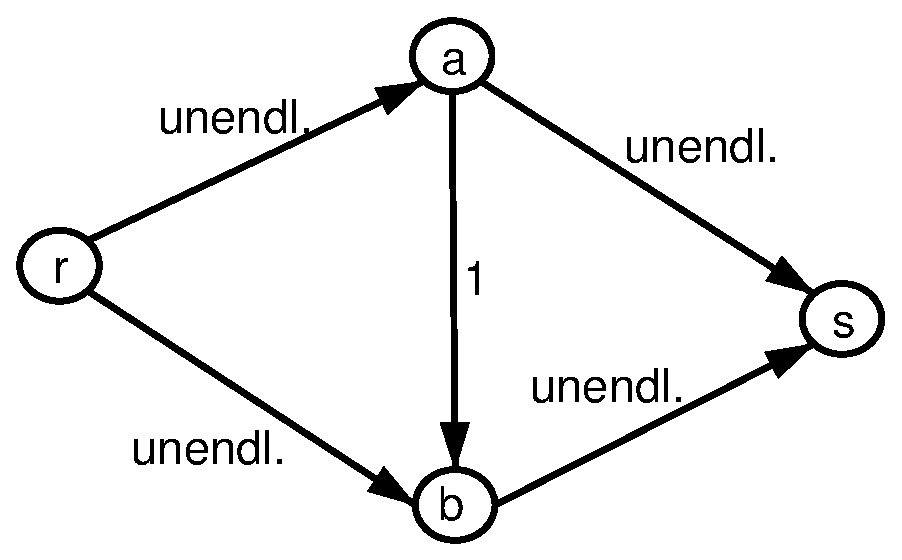
\includegraphics[width=6cm]{bilder/3-0EWTermnicht}

Der Algorithmus wählt immer abwechselnd $r a b s$ und $r b a s \rightarrow$
keine Terminierung wenn $P$ immer über $a b$ geht. Wenn nicht $\infty$
sondern große Zahl $M$, so macht der Algorithmus $M$ Iterationen und hat
einen Fluss von $2M$.\\
$\Rightarrow$ Schranke in \ref{EW} ist scharf

Inputlänge: $n+m+log M$

Ausweg: Kürzeste x-erhöhende, d.h. x-erhöhende Wege mit minimaler
Kantenzahl.

\begin{satz}\label{KEWZeit}
Dinitz [1970], Edmonds und Kasp [1972]\\
Wenn jede Erhöhung auf einem kürzesten, x-erhöhenden Weg statt findet, so
erfolgen höchstens $n \cdot m$ Erhöhungen.
\end{satz}
Beweis: weiter unten nach anderen Sätzen.

\begin{itemize}
\item Keine Annahmen über:
\begin{itemize}
\item Existenz eines maximalen Flusses
\item Rationalität von $u$
\end{itemize}
\item Breitensuche findet einen kürzesten $x$-erhöhenden Weg in Zeit
$O(m)$

Edmonds und Kasp: \begin{quote} "`\ldots so simple that it is likely to be
incorporated innocently into a computer implementation."'
\end{quote}
\end{itemize}

\begin{korollar}\label{ZeitEWA}
Der E-W-Algorithmus mit Breitensuche löst das Max Flow Problem in Zeit
$O(n m^{2})$
\end{korollar}
Zum Beweis von Satz \ref{KEWZeit} zwei Lemmata:

Fluss $x \rightarrow x$-erhöhender Weg $P$ $\underbrace{v_{0}}_{=r}, v_{1},
\ldots, \underbrace{v_{k}}_{=s}$ Fluss $x'$\\
$d_{x}(v,w)$ kürzeste Länge eines $v-w$-Weges in $G(x)$ ($=\infty$ falls
keiner existiert).\\
d.h. $\; d_{x}(r,v_{i}) = i$ \hspace{3mm} $d_{x}(v_{i}, s) = k -i$ $\;\forall\; 0
\leqq i \leqq k$\\
$w v \in E(G(x'))$, $w v \not \in E (G(x)) \Rightarrow (\exists i )\;  w =
v_{i}, \; v = v_{i-1}$

Kante ist jetzt in $G(x')$ da Fluss dort aufgebaut wurde.

\begin{lemma}\label{dxstrichgr}
Für jedes $v \in V$ gilt:
\[d_{x'}(r,v) \geqq d_{x}(r,v)\mbox{ und }d_{x'}(v,s) \geqq d_{x} (v,s)\]
\end{lemma} 
Beweis: Annahme: $(\exists v \in V)\; \; d_{x'}(r,v) < d_{x}(r,v)$\\
Wähle $v$ mit $d_{x'}(r,v)$ Minimum, es gilt $d_{x'} (r,v) > 0 \; \; (v
\not= 0)$\\

Zu $G(x')$: $P'$: $r\underbrace{\rightarrow \; \rightarrow \ldots
\rightarrow}_{\mbox{\scriptsize \begin{tabular}{c}Vorwärts- oder\\
Rückwärtskanten\end{tabular}}}w\rightarrow v$, $w$ ist also der vorletzte Knoten.\\
Länge des Weges $= d_{x'}(r,v)$

Annahme:
\[\begin{array}{rcl}d_{x}(r,v) &>& d_{x'}(r,v)\\
&=&d_{x'}(r,w) + 1 \hspace{3mm} (\ast)\\
&\geqq& d_{x} (r,w) +1 \end{array}\]
$\Rightarrow w v \in E (G(x')) \hspace{5mm} w v \not \in E(G(x))$\\
$\Rightarrow (\exists i ) \; w = v_{i}, \; v=v_{i -1}$\\
$\stackrel{\mbox{\scriptsize$(\ast)$}}{\Leftrightarrow} 
\underbrace{i -1}_{\mbox{
\scriptsize$=$ Distanz von $v=v_{i-1}$}} > \underbrace{i}_{\mbox{
\scriptsize$=$Distanz von $w=v_{i}$}}+1\hspace{3mm}\lightning$\\
$d_{x'}(r,s) \geqq d_{x}(v,s)$ analog q.e.d.

D.h. $\leqq n-1$ Phasen, in jeder Phase: Augmentierungen auf Wegen einer
festen Länge $k$. Frage: Wie oft?
\[E(x):= \{e \in E | e \mbox{ ist Kante eines kürzesten $x$-erhöhenden 
Weges}\}\]

\begin{lemma}\label{KWgroe}
gilt $d_{x'}(r,s) = d_{x}(r,s)$, so gilt $E(x') \subset E(x)$
\end{lemma}
Beweis: Sei $k=d_{x}(r,s) = d_{x'}(r,s)$, $e \in E(x')$\\
$\Rightarrow e = v_{i-1}v_{i}$ oder $e=v_{i}v_{i-1}$ in $x'$-erhöhendem
Weg:
\[P': \; \; \underbrace{\overbrace{v_{0}}^{=v},v_{i},\ldots v_{i-1},}_{
\mbox{\scriptsize$
d_{x'}(r,v)=i-1$}}
\underbrace{v_{i}, \ldots \overbrace{v_{k}}^{s}}_{\mbox{\scriptsize$
d_{x'}(w,s) = k-i$}}\]

$\stackrel{\ref{dxstrichgr}}{\Rightarrow} d_{x}(r,v) + d_{x}(w,s)=k-1$ 

Annahme: $e \not\in E(x) \Rightarrow x_{e} \not= x'_{e} \Rightarrow e \in P
\Rightarrow e \in E(x) \hspace{3mm} \lightning$\\
$\Rightarrow E(x') \subseteq E(x)$

Noch zu Zeigen: $E(x') \neq E(x)$: $\exists e \in P$: $e$ vorwärts und $x'_{e} = u_{e}$ oder $e$ rückwärts und
$x'_{e} = 0$

Annahme: $e \in E(x')$\\
$\Rightarrow$ Jeder $x'$-erhöhende Weg benutzt $e$ anders herum als in
$P$\\
$ (\exists i)$ Länge von $P' > -\underbrace{i}_{\mbox{\scriptsize$r
\ldots v_{i}$}} + \underbrace{k-i+1}_{\mbox{\scriptsize $v_{i-1}\ldots s$}} +
 \underbrace{1}_{v_{i}\ldots v_{i-1}} = k+2 \hspace{3mm}\lightning$\\
$\Rightarrow e \not\in E(x')$

Anschaulich: $e$ ist der Flaschenhals von $P$.

Beweis von Satz \ref{KEWZeit}:\\
Lemma \ref{dxstrichgr} $\Rightarrow$ höchstens $n-1$ Phasen\\
Lemma \ref{KWgroe} $\Rightarrow$ höchstens $m$ Erhöhungen pro Phase\\
$\Rightarrow m n$ Erhöhungen. q.e.d.

D.h. Gesamtlaufzeit für kürzeste erhöhende Wege Algorithmus $O(n m^{2})$.
Später noch ein Algorithmus mit Laufzeit $O(n^{2}m)$.

\section{Anwendungen von Max Flow Min Cut}

\subsection{Bipartite Matchings und Knotenüberdeckungen}
Bipartite Graphen $G(V,E)$ ungerichtet\\
$V=P \cup Q$ \hspace{3mm} $E = \{p q| p \in P, q \in Q\}$\\
$P \cap Q = \varnothing$ \hspace{3mm} $\{P,Q\}$ Bipartition der Graphen.

Bsp:


\includegraphics[height=2cm]{bilder/3-0BipMatch}

\paragraph{Bipartites Matching} $M$\\
$M \subseteq E$ mit keine zwei kanten in M haben einen gemeinsamen
Endknoten, b.z.w. $(\forall \; v \in V) | \{ e \in M | v \in e\}| \leqq 1$

Im Beispiel z.B: 


\includegraphics[height=2cm]{bilder/3-0BipMatch2}

\paragraph{Heiratsproblem} \mbox{}\\

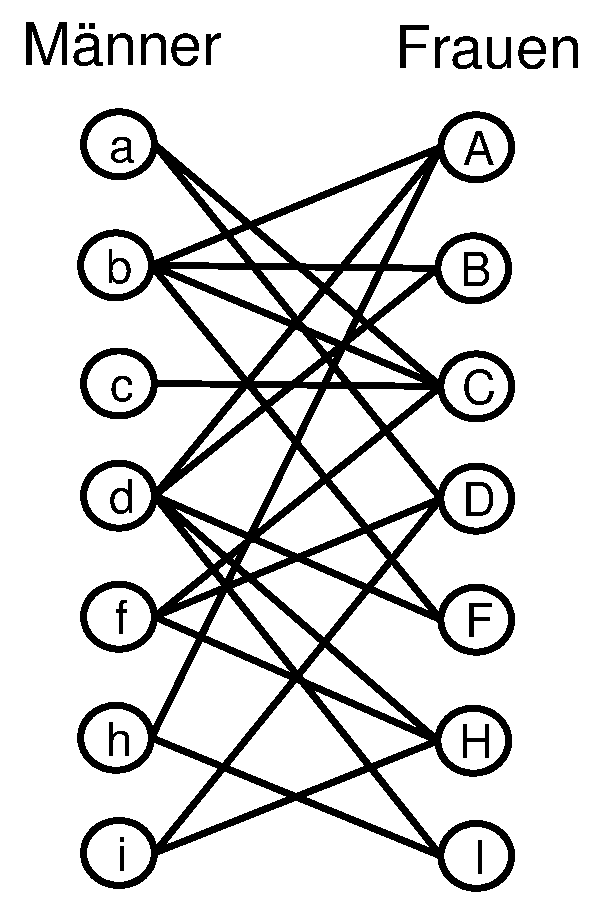
\includegraphics[height=4cm]{bilder/3-0Heiraten}

Hierbei verdeutlichen die Kanten ein "`sich mögen"' und es sollen möglichst
viele Paare verheiratete werden aber nur solche die sich mögen. Eine Lösung
ist:

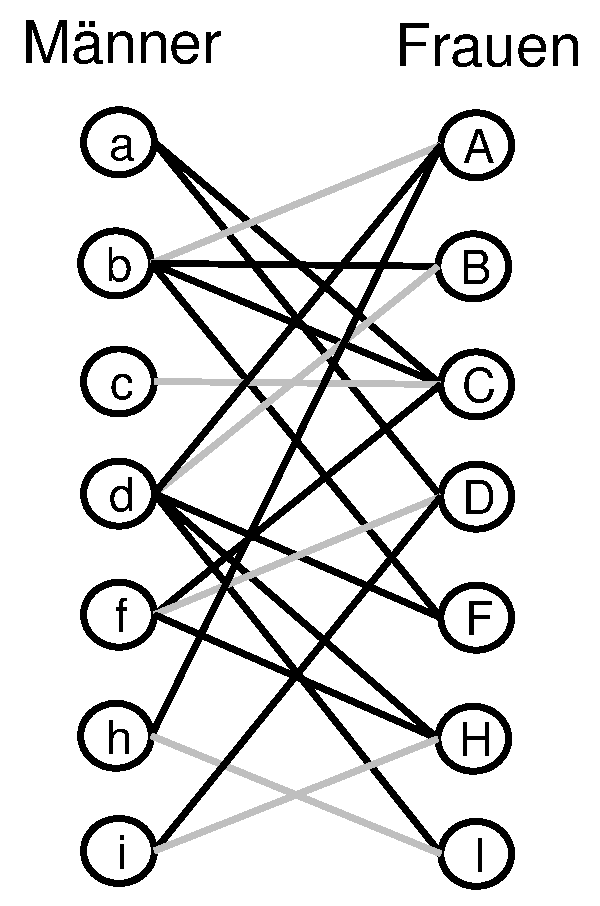
\includegraphics[height=4cm]{bilder/3-0Heiraten2}

Hierbei können also sechs Paare verheiratet werden, wären auch mehr
möglich?

$C \subseteq V$ heißt Knotenüberdeckung falls:
\[ (\forall v w \in E) \; v \in C \mbox{ oder }w \in C\]
Offensichtlich handelt es sich hier um Schwache Dualität.\\
$M$ Matching im bipartiten Graphen $G=(V,E)$\\
$C$ Knotenüberdeckung im bipartiten Graphen $G=(V,E)$\\
$\Rightarrow |M| \leqq |C|$\\

nun die Knotenüberdeckung (grau gefärbte Knoten:)

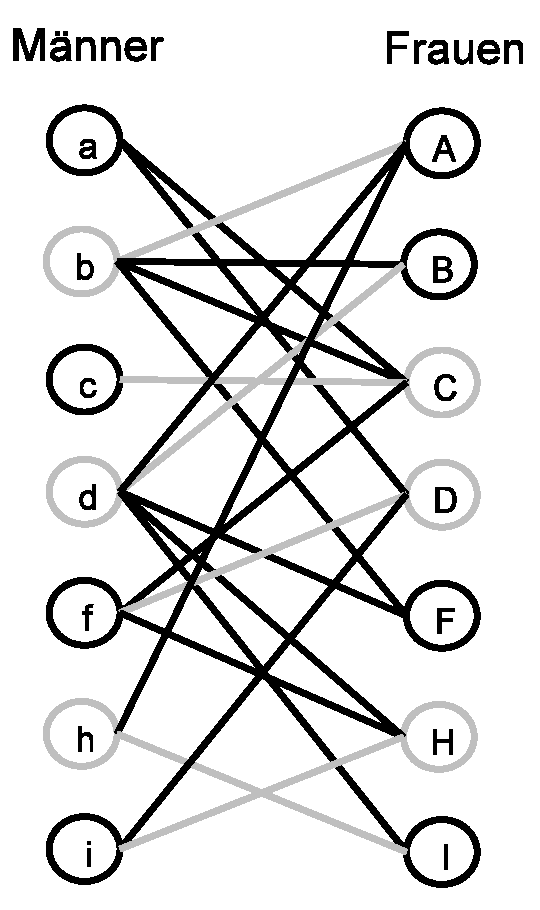
\includegraphics[height=4cm]{bilder/3-0Heiraten3}

Diese hat nun auch 6 Knoten also ist die Lösung auch optimal:\\
$6=\max |M| = \min |C|$

\begin{satz}
Satz von König [1931]\\
Für bipartite Graphen $G=(V,E)$ gilt:\\
\[ \max \{ |M| | \mbox{ ist Matching } \} = \min \{ |C|| \mbox{
ist Knotenüberdeckung } \}\]
\end{satz}
Beweis: Aus ungerichtetem Graphen $G=(V,E)$ konstruieren wir einen
gerichteten Graphen $G'(V',E')$ wie folgt:\\
$ V':= V \cup \{r,s\} \hspace{5mm} E': \forall p q \in E,\; p \in P, q \in
Q$ gerichtete Kanten $p q \in E'$ mit der Kapazität $u_{p q} = \infty$,
zusätzlich $\forall p \in P$ gerichtete Kante $r p$ mit Kapazität $u_{r p}=1$
und $\forall q \in Q$ gerichtete Kante $q s$ mit Kapazität $u_{q s}= 1$

Im Beispiel:

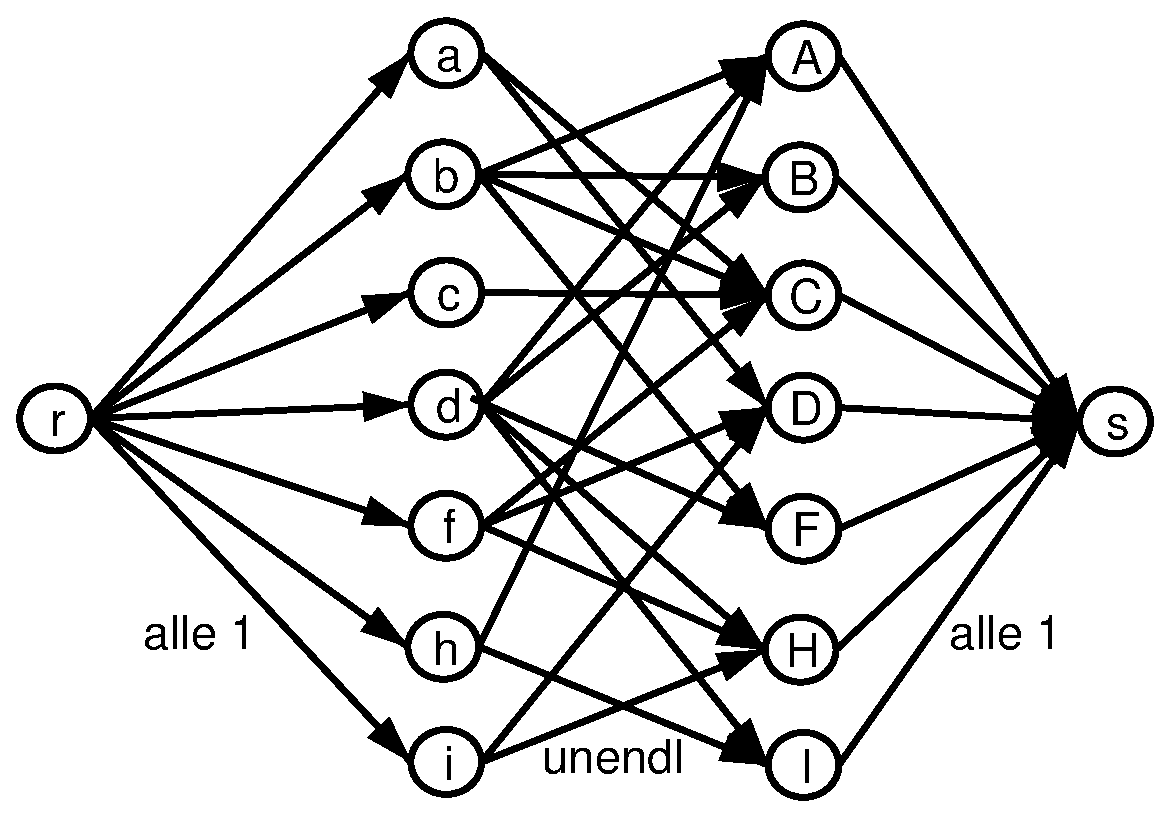
\includegraphics[height=4cm]{bilder/3-0Heiraten4}

Sei $x$ ein ganzzahliger (d.h. 0/1) Fluss in $G'$ mit Flusswert $k$.\\
Wir definieren $M\subseteq E$ durch:
\[\mbox{Für $p q \in E$ gilt } \left\{ \begin{array}{l}
p q \in M \; \mbox{ falls } x_{p q}=1\\
p q \not \in M \mbox{ falls } x_{p q} = 0\\
\end{array} \right.\]
Dann ist $M$ ein Matching in $G$ mit Kardinalität $k$.

Umgekehrt: Sei $M$ ein Matching in $G$ mit Kardinalität $k$.\\
Wir definieren $x_{v w}$ für $v w \in E'$ durch:
\[\begin{array}{ll}
v \in P , \; w \in Q&: x_{v w} = \left\{\begin{array}{l}
1 \mbox{ falls } v w \in M\\
0 \mbox{ falls } v w \not\in M\\
\end{array} \right.\\
v = r, \; w \in P&: x_{v w} = \left\{\begin{array}{l}
1\; (\exists e \in M) \; w \in e\\
0 \mbox{ sonst}\\
\end{array} \right.\\
v \in P, \; w=s&: x_{v w} = \left\{\begin{array}{l}
1\; (\exists e \in M) \; v \in e\\
0 \mbox{ sonst}\\
\end{array} \right.
\end{array}
\]
Dann ist $x$ ein ganzzahliger zulässiger Fluss in $G'$ mit Flusswert $|M|$.

D.h. wir können das maximale Kardinalität Matching mit Max-Flow Berechnung
bestimmen mit höchstens $\min \{|P|,|Q|\} \leqq n$ Flusserhöhungen. Satz
\ref{EW} liefert uns die Laufzeit $O(m n)$ Sei $\delta'(\{r\} \cup A)$ mit
$A \subseteq V$ ein minimaler $(r,s)$-Schnitt in $G'$

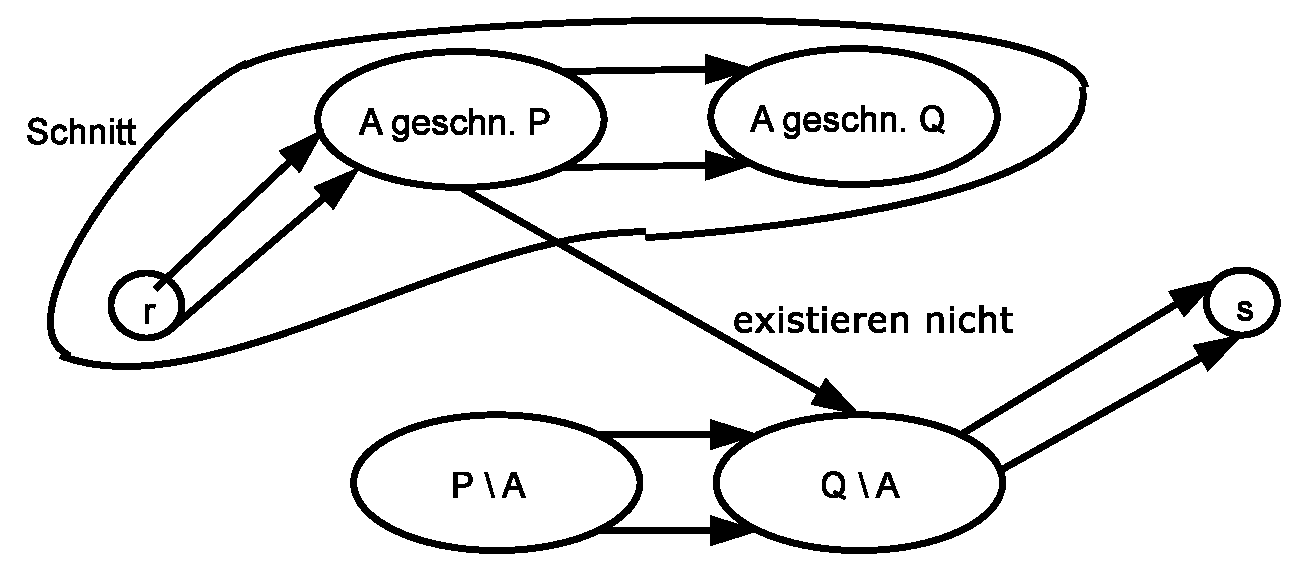
\includegraphics[height=3cm]{bilder/3-0MinKnotenueber}

Endliche Kapazität des Schnitts $\Rightarrow (\nexists v w \in G) \; v
\in  A \cap P, \; w \in Q \wout A$.\\
$\Rightarrow$ Jede Kante $e \in G$ ist inzident zu einem Knoten in $C := (P
\wout A) \cup (Q \cap A)$\\
$\Rightarrow C$ ist Knotenüberdeckung mit Kardinalität $|C| = |P \wout
A| + | Q \cap A| = $ Kapazität des Schnitts $= \max \{|M|| M \mbox{
Matching} \}$\\
D.h. der Algorithmus kann auch eine minimale Knotenüberdeckung berechnen. 

\subsection{Transportproblem}

Gegeben: bipartiter Graph $G=(V,E)$, $V=P\cup Q$, $a\in \ZZ^{P}_{+}$, $b \in
\ZZ^{Q}_{+}$\\
Gesucht: $x \in \RR^{e}$ mit:
\[\begin{array}{rcl}
\displaystyle \sum_{q \in Q, \; p q \in E}x_{p q}&\leqq& a_{p} \; \forall p \in
P\\
\displaystyle \sum_{p \in P, \; p q \in E} x_{p q} = b_{q}\\
x_{p q} &\geqq& 0 \; \forall p q \in E\\
x_{p q}&& \mbox{ganzzahlig } \forall \; p q \in E\end{array}
\]
Nun ist gefragt ob alle Nachfragen $b$ mit den gegebenen Kapazitäten $a$
überhaupt befriedigt werden können. Mathematisch ist also gefragt, ob
eine zulässige Lösung für das Problem existiert. Auch dieses Problem
ähnlich wie das Matching-Problem wird auf ein Max-Flow Problem übertragen:
Beispiel:

\begin{tabular}{c@{\hspace{5mm}}c}
Transportproblem&Flussproblem\\
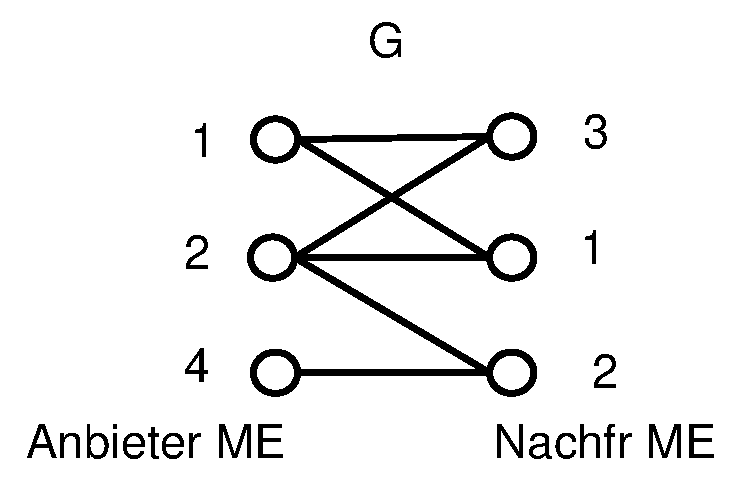
\includegraphics[height=3cm]{bilder/3-0Transport1}&
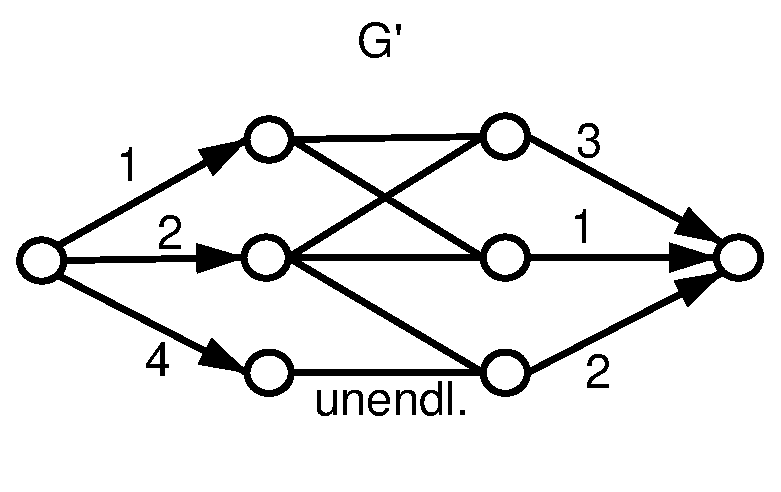
\includegraphics[height=3cm]{bilder/3-0Transport2}\\
$\exists$ Lösung $x\in \ZZ^{E}$ & $\Leftrightarrow \exists$ ganzzahliger
zul. Fluss mit Wert $\displaystyle \sum_{q\in Q} b_{q}$
\end{tabular}

Nach der Umformung kann man einfach den Max-Fluss Algorithmus anwenden:\\
Max-Flow-Min-Cut Theorem:\\
(TB) hat Lösung genau dann wenn jeder $(r,s)$-Schnitt in $G'$ als maximale
Kapazität wenigstens $\displaystyle \sum_{q\in Q} b_{q}$ hat.

Für $A \subseteq P$, $B \subseteq Q$ ist die Kapazität des Schnitts:
\[ \delta'(A\cup B \cup \{r\}) = \sum_{i \in P\wout A} a_{i} +
\sum_{j\in B} b_{j}\]

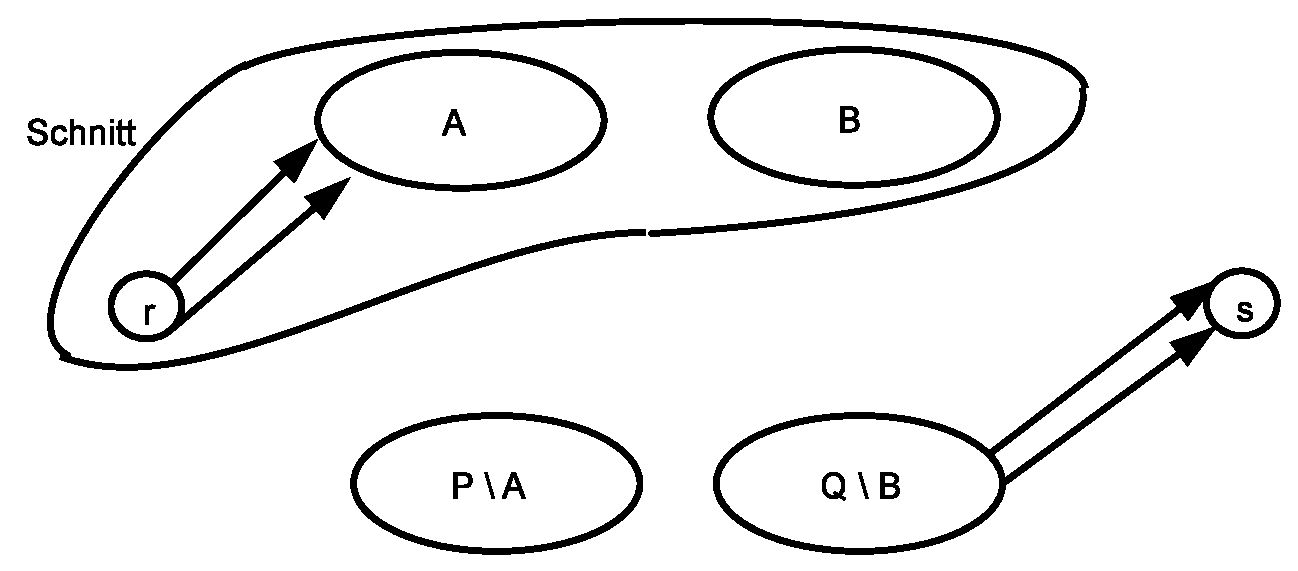
\includegraphics[height=4cm]{bilder/3-0TransportSchnitt}

\[\sum_{i \in P\wout A} a_{i} + \sum_{j \in B} b_{j} \geqq \sum_{q \in Q}
b_q \mbox{ g.d.w. }  \sum_{i \in P \wout A} a_{i} \geqq \sum_{j = Q \wout
B} b_{j}\]
Wir können die Überprüfung beschränken auf solche $A \subseteq P$ für die
gilt: Jeder Knoten aus $P \wout A$ ist mit einem Knoten aus $Q \wout B$
adjazent.

Für $C \subseteq V$:
\[N(C) := \{w \in V | v w \in E \mbox{ für ein v } \in C\} =
(\mbox{ungerichtete Nachbarmenge}) \]
also können wir annehmen:
\[N(Q \wout B) = P \wout A\]
Fazit:
\begin{satz}
$\exists$ Lösung für (TB) genau dann wenn $(\forall \; C \subseteq Q)
\hspace{3mm} a(N(C)) \geqq b(C)$
\end{satz}

Interpretation: Für jede Kundenteilmenge muss der Bedarf durch die
möglichen Produzenten gedeckt sein.

\section{Minimale Schnitte und lineare Optimierung}

Max-Fluss Problem als LP
\[\begin{array}{lrcl}
(LPMF)& \max \displaystyle \sum_{w \in V,\; w s \in E} x_{w s} -
\sum_{w \in V, \; s w \in E} x_{s w}\\
(y_{v})& \displaystyle \sum_{w \in V, \; w v \in E} x_{w v} - \sum_{w \in V,
\; v w \in E} x_{v w}&=& 0 \; \; \forall \; v \in V \wout \{r,s\}\\
(z_{v w})& x_{v w } &\leqq& u_{v w} \; \; \forall \; v w  \in E\\
&x_{v w} &\geqq & 0 \; \; \forall \; v w \in E
\end{array}
\]
Duales LP
\[\begin{array}{lrcl}
(DLPMF)& \min \displaystyle \sum_{v w \in E} u_{v w} z_{v w}\\
&-y_{v} + y_{w} + z_{v w } &\geqq &0 \; \; \forall \; v w \in E, \; v,w \in
V \wout \{r,s\}\\
&y_{w} + z_{r w} &\geqq& 0 \; \; \forall \; r w \in E\\
&-y_{v} + z_{v r} &\geqq& 0 \; \; \forall \; v r \in E\\
&-y_{v} + z_{v s} &\geqq& 1 \; \; \forall \; vs \in E\\
&y_{w} + z_{s w} &\geqq& -1 \; \; \forall \; s w \in E\\
&z_{v w } &\geqq& 0 \; \; \forall \; v w  \in E
\end{array}\]

Vereinfachung durch setzen der neuen Dualvariablen:
\[ y_{r}=0 \hspace{7mm} y_{s} = -1\]
erhalten wir die gemeinsame Form:
\[ -y_{v} + y_{w} + z_{v w} \geqq 0 \; \; \forall \; v w \in E\]

Die Addition von 1 zu allen $y_{v} \; (v \in V)$ ändert die Restriktion
nicht, also ist (DLPMF) äquivalent zu:

\[\begin{array}{lrcl}
(DLPMF')& \min \displaystyle \sum_{v w \in E} u_{v w} z_{v w}\\
&y_{r} &=& 1\\
&y_{s} &=& 0\\
&-y_{v} + y_{w} + z_{v w} &\geqq& 0 \; \;  \forall \; v w \in E\\
&z_{v w} &\geqq & 0 \; \; \forall \; v w \in E
\end{array}\]

\begin{satz}
Falls (DLPMF') eine Optimallösung hat, so hat (DLPMF') eine Optimallösung
 der folgenden Form:\\
Für einen $(r,s)$-Schnitt $\delta(R)$ ist $y$ der charakteristische Vektor
von $R$ und $z$ der charakteristische Vektor von $\delta(R)$
\end{satz}

Beweis:\\
Wähle $\delta(R)$ MIT $r \in R$ als minimalen Schnitt und $y,z$ als die
entsprechenden charakteristischen Vektoren. Dann gilt:

\[ y_{r} = 1, \; \; y_{s} = 0, \; \; z_{v w } \geqq 0 \; \; \forall v w
\in E\]
und:

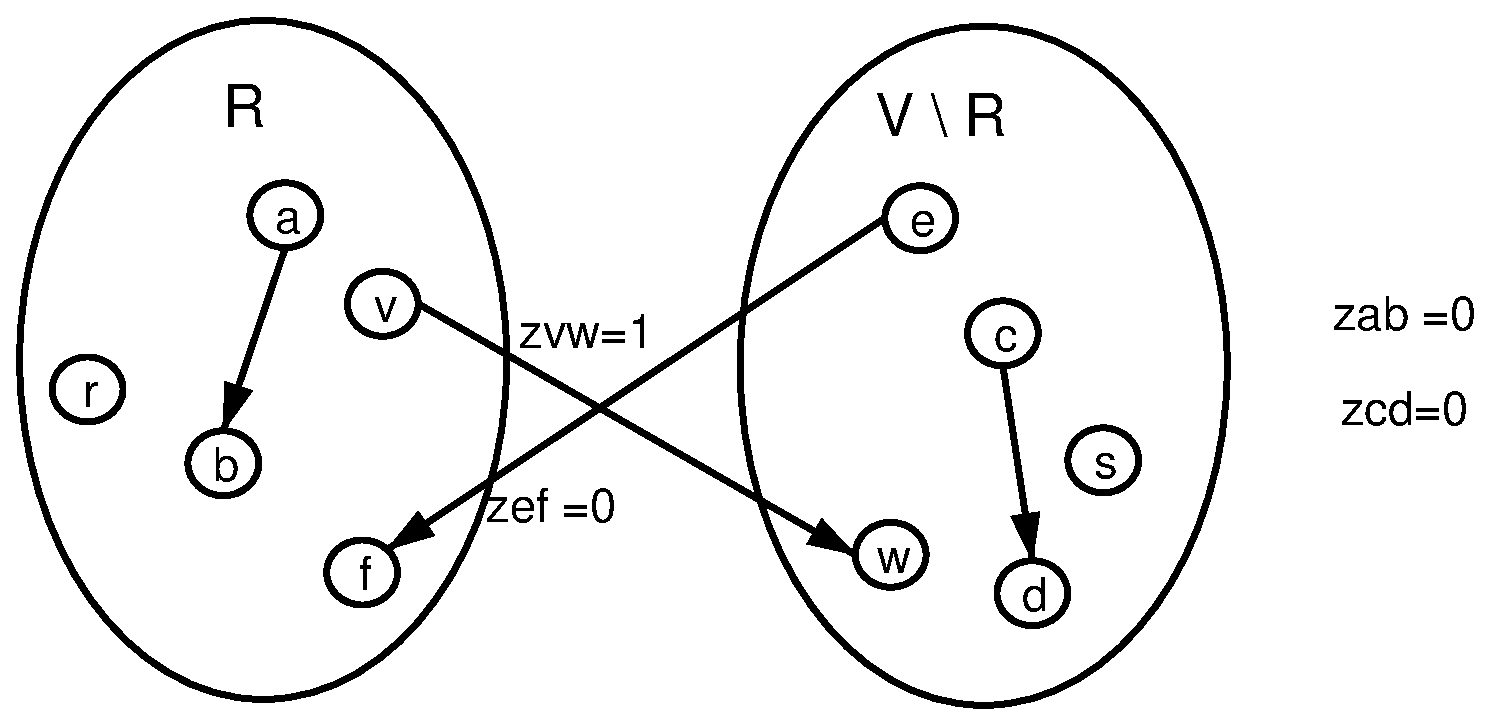
\includegraphics[height=4cm]{bilder/3-0DLPMF}

\[\begin{array}{rcl@{\hspace{5mm}}rcl}-y_{a }- y_{b} + z_{a b}&&&
-y_{c} + y_{d} - z_{c d}\\
-1 + 1 +0 &=&0&=0+0+0&=&0\vspace{2mm}\\
-y_{v}+y_{w}+z_{w}&&&-y_{e}+y_{f}+z_{e f}\\
=-1+0+1&=&0&=0+1+0&>&0\\
\end{array}\]

Somit ist $y_{z}$ zulässig für (DLPMF') und der ZF-Wert ist:

\[\begin{array}{rcl}
\displaystyle \sum_{v w \in E} u_{v w} z_{v w } &=& u(\delta(R))\\
&\stackrel{\mbox{\scriptsize Max-Flow-Min-Cut}}{=}&\mbox{Wert des max.
Flusses}\\
&=& \mbox{Optimaler Wert (LPMF)}\\
&\stackrel{\mbox{\scriptsize Dualitätsth.}}{=}& \mbox{Optimaler Wert von
(DLPMF')} 
\end{array}\] 

\subsubsection{Formulierung des minimalen Schnitt Problems ohne y-Variable}

\[\begin{array}{rrcl}
(LPMC)\hspace{7mm}& \min \displaystyle \sum_{e \in E} u_{e} z_{e}\\
\mbox{s.t.}& \displaystyle \sum_{e\in P} z_{e} &\geqq& 1 \; \; \forall \;
\mbox{einfache $(r,s)$-Wege $P$}\\
&z_{e} &\geqq&0 \; \; \forall \; e \in E \end{array} 
\]
Offensichtlich: Jeder charakteristische Vektor eines $(r,s)$-Schnittes
$\delta(R)$ $z_{e}=\left\{ \begin{array}{l}\mbox{1 falls $e \in \delta(R)$}\\
\mbox{0 sonst}\end{array}\right.$ ist zulässig für (LPMC).
\begin{satz}
Falls (LPMC) eine Optimallösung hat, so hat (LPMC) eine Optimallösung, die
charakteristischer Vektor eines $(r,s)$-Schnittes ist.
\end{satz}
Beweis: Wäre $u_{e} < 0$ für ein $e \in E$, so wäre (LPMC) unbeschränkt,
also gilt: $u_{e} \geqq 0 \; \forall \; e \in E$\\
Sei $z'$ charakteristischer Vektor eines minimalen $(r,s)$-Schnittes
$\delta(R)$. Das duale LP lautet:
\[\begin{array}{rrcl}
(DLPMC)\hspace{7mm}& \max \displaystyle \sum_{P \mbox{ einf. $(r,s)$-Weg }}
w_{P}\\
\mbox{s.t.}&\displaystyle \sum_{P} w_{P} &\leqq & u_{e} \; \; \forall \; e \in E\\
&w_{P} &\geqq & 0 \; \; \forall \mbox{ einf. $(r,s)$-Wege } P \end{array}
\]
Sei $x$ ein maximaler Fluss mit Wert $F$.\\
Wiederhole:\\
Finde einfachen $(r,s)$-Weg $P$ der Form:
\[r\stackrel{x_{e_{1}}>0}{\longrightarrow}\bullet
\stackrel{x_{e_{2}}>0}{\longrightarrow}\bullet\longrightarrow \ldots
\stackrel{x_{e_{k-1}}>0}{\longrightarrow}\bullet
\stackrel{x_{e_{k}}>0}{\longrightarrow}s\]
Setze $w_{p} := \min\{x_{e_{i}} | 1 \leqq i \leqq k\}$\\
Setze für $1 \leqq i \leqq k: \; x_{e_{i}} := x_{e_{i}} -w_{p}$ bis $f_{x} = 0$. Nun gilt $\displaystyle \sum_{P} w_{p} = F$\\
Die Prozedur terminiert, da immer wenigstens ein $x_{e}$ Null wird.\\
$w$ ist zulässig für (DLPMC) und 
\[\sum_{P} w_{p} = \sum u_{e} z'_{e}\]
$\Rightarrow z'$ ist optimal für (LPMC)

\section{Der Algorithmus von Goldberg und Tarjan [1988]}
Vereinbarung: Falls $v w \in E$ und $ w v \not\in E$ setzen wir $u_{w v} =
x_{w v}=0$ (nur für Beschreibung des Algorithmus, die Implementierung fügt
Kante nicht hinzu).

Für $x \in R^{e}$ (nicht notwendigerweise Fluss) mit $0 \leqq x_{e} \leqq
u_{e} \; \forall \; e \in E$ definieren wir den Hilfsdigraphen $G(x)$.\\
$v w \in E(G(x)) \Leftrightarrow x_{v w} < u_{v w}$ oder $x_{w v} > 0$.
Parallele Kanten in $G(x)$ sind nicht erlaubt.

Restkapazität von $v w$: $\bar{u}_{v w} := u_{v w } - x_{v w} + x_{w v}$\\
($\bar{u}_{v w}$ kann auf $v w$ zusätzlich fließen ohne $0 \leqq x_{v w}
\leqq u_{v w}$ zu verletzen. Eine solche Lösung verletzt im Allgemeinen aber
die Flusserhaltungsbedingung)

$x$ heißt Präfluss (Preflow) falls:
\[f_{x}(v) \geqq 0 \; \; \forall \; v \in V \wout \{r,s\}\]

\paragraph{Push Operation} für $v w \in E$ mit $\bar{u}_{v w} > 0$ und
$f_{x}(v)>0$ 
\[x_{v w}\ \leftarrow x_{v w} + \underbrace{\min (\bar{u}_{v w},\; f_{x}(v))
}_{:= \epsilon}\]
Erhält die "`zulässiger Präfluss"' Eigenschaft. (Falls auch $w v \in E$ und
$\epsilon < \bar{u}_{v w })$\\
\[\begin{array}{rcl}
x_{w v} &\leftarrow& x_{w v} - \underbrace{\min(\epsilon, \; x_{w v})}_{ :=
\epsilon'}\\
x_{v w} &\leftarrow & x_{v w} + \epsilon - \epsilon'\end{array}
\]

Beispiel:

\begin{tabular}{l}
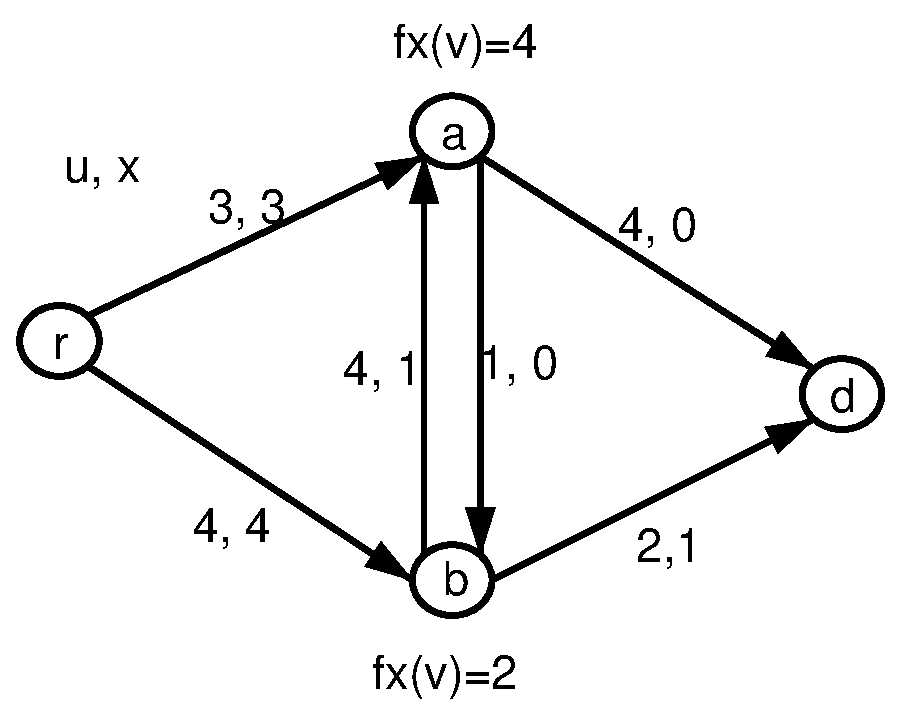
\includegraphics[height=3cm]{bilder/3-0Praefluss1}
\end{tabular}
$\stackrel{\mbox{push}(a,b)}{\Longrightarrow}$
\begin{tabular}{l}
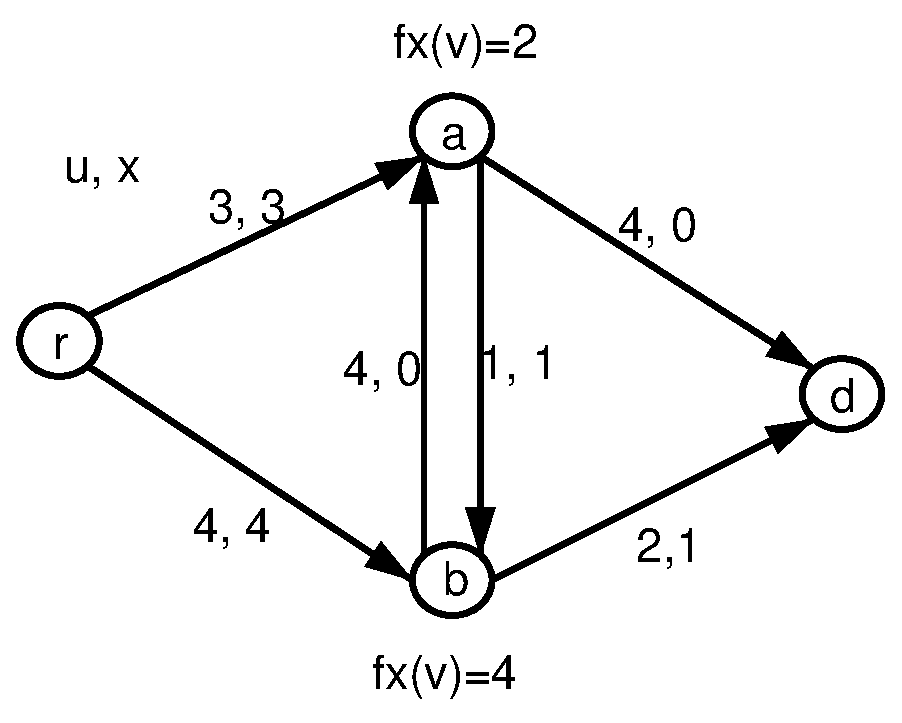
\includegraphics[height=3cm]{bilder/3-0Praefluss2}
\end{tabular}


Zu erkennen ist dass hier auch die "`zulässiger Präfluss"' Eigenschaft
erhalten bleibt.\\
Knoten $v \in V \wout \{r,s\}$ ist {\em aktiv} falls $f_{x}(v) > 0$\\
$\Rightarrow$ Ein Präfluss ist ein Fluss, falls es keine aktiven Knoten
gibt.

Grundoperationen:
\begin{enumerate}
\item Wähle einen aktiven Knoten $v$
\item Wähle $v w \in G(x)$
\item push $v w$
\end{enumerate} 
Wesentlich ist die richtige Reihenfolge, sonst könnte der Algorithmus
unendlich operieren: push$(v w)$, push$(w v)$, push$(v w)$, push$(w v),
\ldots$

$d \in (\ZZ^{+} \cup \{\infty\})^{V}$ ist eine gültige Nummerierung (valid
labeling) bezüglich eines Präflusses $x$ falls:
\[\begin{array}{rcl}
d(r)&=&n\\
d(s)&=& 0\\
d(v) &\leqq& d(w) +1 \; \; \forall \; v w \in G(x)  
\end{array}\]

Invariante des GT-Algorithmus: Zulässiger Präfluss mit gültiger Nummerierung.

{\bf Initialisierung:}\\
Initialisiere $(x,d)$;\\
$\forall \; i j \in E$ setze  $x_{i j} = \left\{ \begin{array}{l}u_{i j}, \mbox{
falls } i=r\\ 0 \mbox{ sonst}\end{array} \right.$\\
$\forall \; i \in V$ setze $d_{i} = \left\{ \begin{array}{l}n, \mbox{
falls } i=r\\ 0 \mbox{ sonst}\end{array} \right.$

$x$, $d$ erfüllen gültige Nummerierung (wir müssen annehmen, dass alle
$u_{r v} < \infty$ falls nicht, so kann man diese Bedingung herstellen. In
der Übungsaufgabe...)

Beispiel:

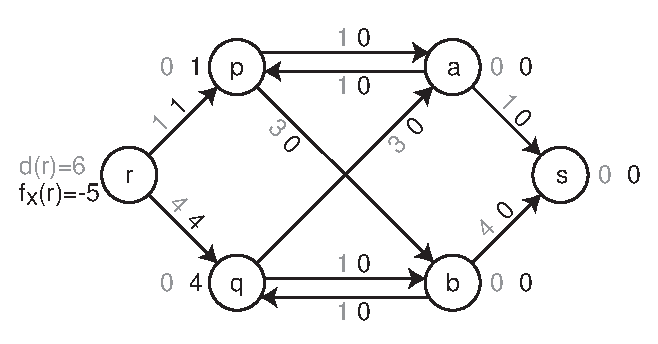
\includegraphics[height=4cm]{bilder/3-0GoldbTarjan}

\begin{lemma}
Ist $x$ ein zulässiger Präfluss und $d$ eine gültige Nummerierung bezüglich
$x$, so existiert ein $(r,s)$-Schnitt $\delta(R)$, so dass\\
\[\begin{array}{rcl}
x_{v w}&=& u_{v w} \; \; \forall \; v w \in \delta(R)\\
x_{v w}&=& 0 \; \; \forall \; v w \in \delta(\bar{R})
\end{array}\]
\end{lemma}
Beweis: In einer gültigen Nummerierung $\exists k, \; 0 < k < n, \; d(v)
\not= k \forall \; v \in V$ ($n-1$ Zahlen auf $n-2$ Knoten, einer bleibt
über)\\
Setze $R:= \{v \in V | d(v) > k\}$\\
dann ist $r \in R, \; s \not\in R$ und wegen gültiger Nummerierung kann
keine Kante in $G(x)$ $R$ verlassen $\Rightarrow$ Behauptung.

\begin{korollar}\label{GueltmaxFluss}
Hat ein zulässiger Fluss eine gültige Nummerierung, so ist $x_{e}$ ein
maximum Fluss.
\end{korollar}
Korollar \ref{GueltmaxFluss} liefert Terminierungsbedingung.
Invariante:
\begin{enumerate}
\item zulässiger Präfluss
\item gültige Nummerierung (d.h. saturierter Schnitt)
\end{enumerate} 
Terminierung sobald Fluss.

vgl. Erhöhender Wege-Algorithmus:
Invariante:
\begin{enumerate}
\item zulässiger Fluss
\item Terminierung, sobald ein Schnitt saturiert ist.
\end{enumerate}
Die gültige Nummerierung approximiert Distanzen in $G(x)$
\begin{lemma}
Für jeden zulässigen Präfluss $x$ und jede gültige Nummerierung $D$
bezüglich $x$ gilt:
\[d_{x}(v,w) \geqq d(v) - d(w) \; \; \forall v, w \in V\]
\end{lemma}
Beweis: für $d_{x}(v,w) = \infty$ trivial.\\
für $d_{x}(v,w) < \infty$, $P$ ein kürzester gerichteter (v,w)-Weg in
$G(x)$.\\
Wir addieren die Ungleichungen $d(p) - d(q) \leqq 1$ für alle $p q \in P$.
\\ Summe: $d(v) - d(w)$ q.e.d.

Insbesondere gilt:
\[\begin{array}{rcl}d(v) &\leqq& d_{x}(v,s)\\
d(v)-n &\leqq & d_{x}(v,r)\end{array}\]
Also $d(v) \geqq n \Rightarrow d_{x}(v,s) = \infty$\\
D.h. in diesem Fall sollte der Fluss Richtung Quelle "`gepusht"' werden.

\paragraph{Strategie}: $push(v w)$ mit $d(w) < d(v)$\\
\[\left.\begin{array}{l}
\mbox{gültige Nummerierung}\\
v w \in G(x)\\
d(w) < d(v)\end{array} \right\}\rightarrow d(w) = d(v) -1\]
$v w$ eine {\em zugelassene Kante} (admissible arc) falls $v w \in E(G(x)), d(v) =
d(w) +1$\\
Ein $push(v w)$ auf $v w$ erhält die gültige Nummerierung. $w v$ könnte in
$E(G(x'))$ sein, aber $d(w) \leqq d(v)+1$ gilt bereits vorher.

Was ist aber nun wenn $v$ aktiv ist aber $(\nexists v w \in G(x)) \; d(v) =
d(w) +1$? Antwort: $relabel(v)$: $d(v) \leftarrow min\{d(w) +1| v w \in
E(G(x))\}$.

Auch danach ist die Nummerierung in $G(x)$ noch gültig:

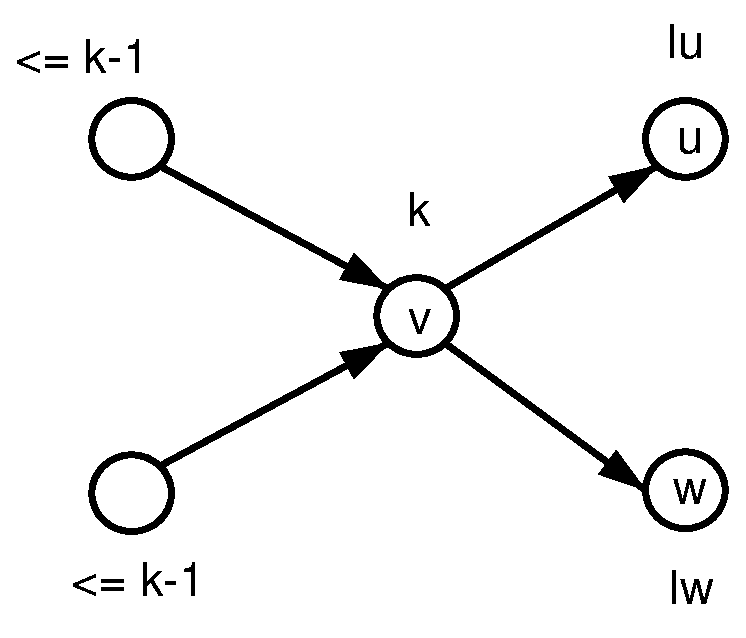
\includegraphics[height=3cm]{bilder/3-0PushOp}
\\$\begin{array}{l}l_{u} \geqq k -1\\
\mbox{hier: }l_{u}\ \geqq k\\
l_{w} \geqq k -1\\
\mbox{hier: }l_{w}\geqq k\end{array}$

Wenn $l_{w}$ Minimum ist, dann erhält $v$ also die Nummer $l_{w}+1$

$process(v)$
\begin{algorithmic}
\WHILE{$\exists$ zugelassene Kante $v w$}
\STATE $push(v w)$;
\IF{$v$ aktiv}
\STATE $relabel(v)$
\ENDIF
\ENDWHILE
\end{algorithmic}

\paragraph{Der Goldberg-Tarjan Algorithmus} \mbox{}\\
\begin{algorithmic}
\STATE initialize $(x,a)$;
\WHILE{$x$ is not a flow}
\STATE choose active node $v$;
\STATE $process(v)$
\ENDWHILE
\end{algorithmic}

Beispiel: Wir wählen immer $v$ mit größter Distanz $d(v)$ "`maximum
distance"'-Version des GT-Algorithmus. 
%Vielen Dank an Prof. Jünger dafür,
%dass er freundlicherweise Scans der Zeichnungen zur Verfügung gestellt hat.
Vielen Dank an Daniel Teske für die Zeichnungen...

An den Knoten sind die grauen Zahlen die Distanzlabel, die dunklen
Nettofluss/Überschuss, an den Kanten sind die Kapazitäten hell und der
Fluss dunkel.

%\begin{tabular}{ccc}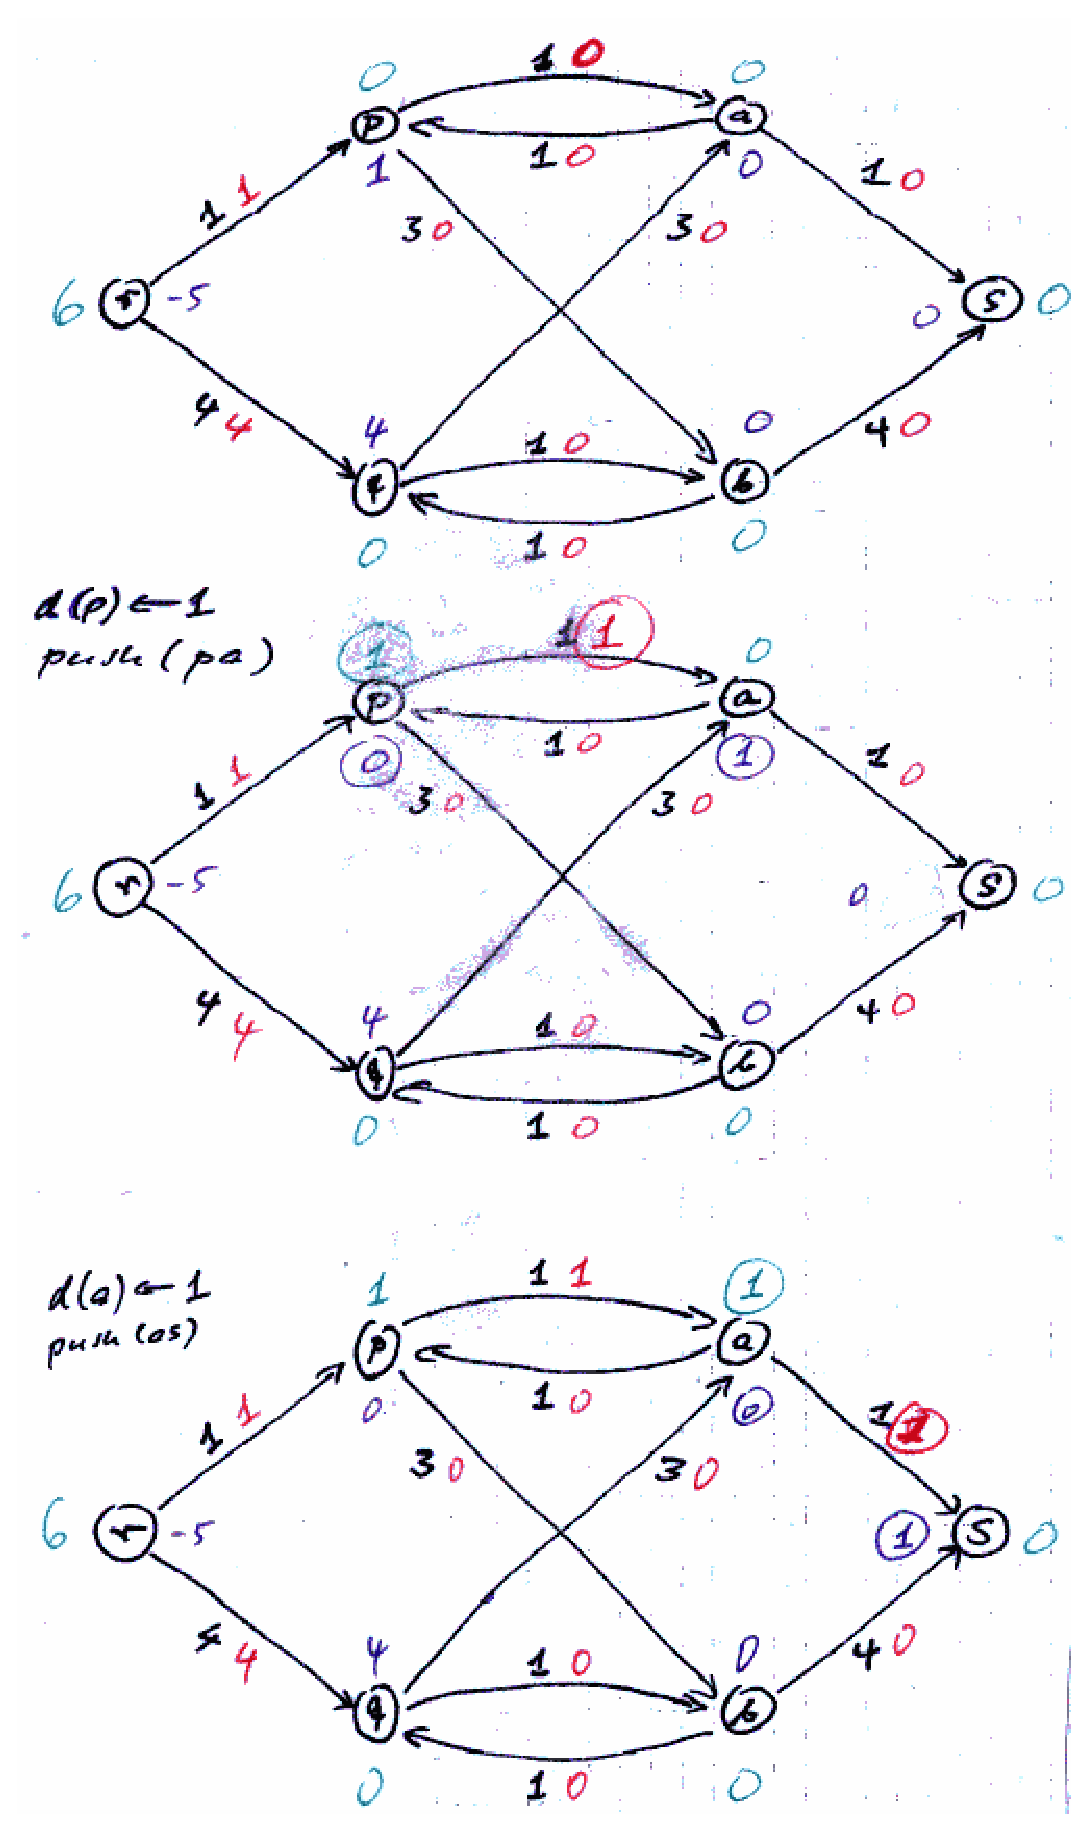
\includegraphics[width=5cm]{bilder/3-0Tarjan1}
%&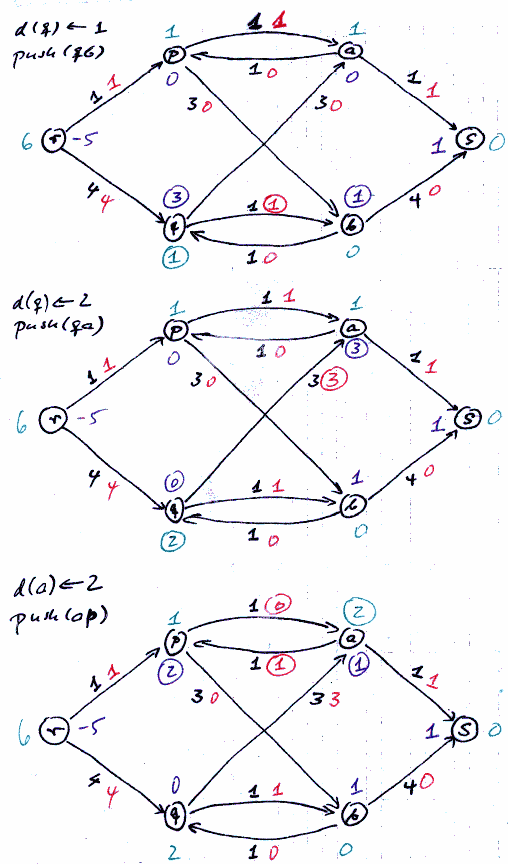
\includegraphics[width=5cm]{bilder/3-0Tarjan2}
%&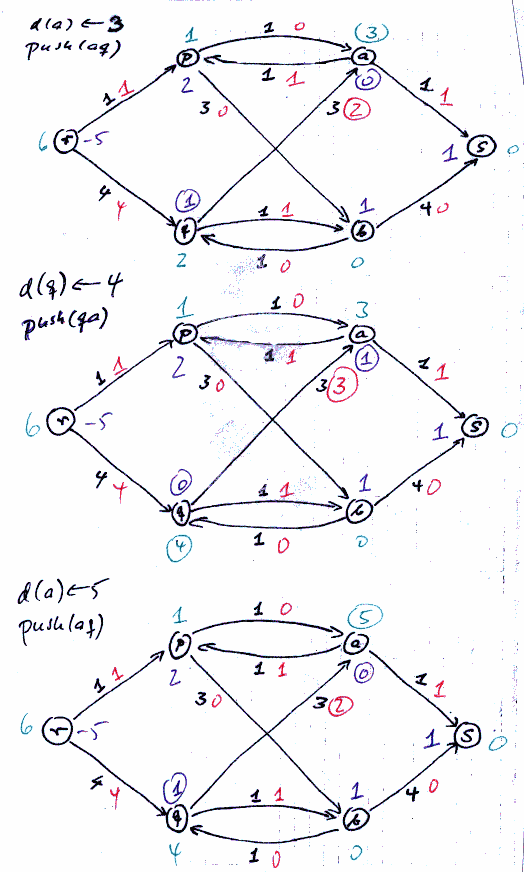
\includegraphics[width=5cm]{bilder/3-0Tarjan3}\end{tabular}

%\begin{tabular}{cc}
%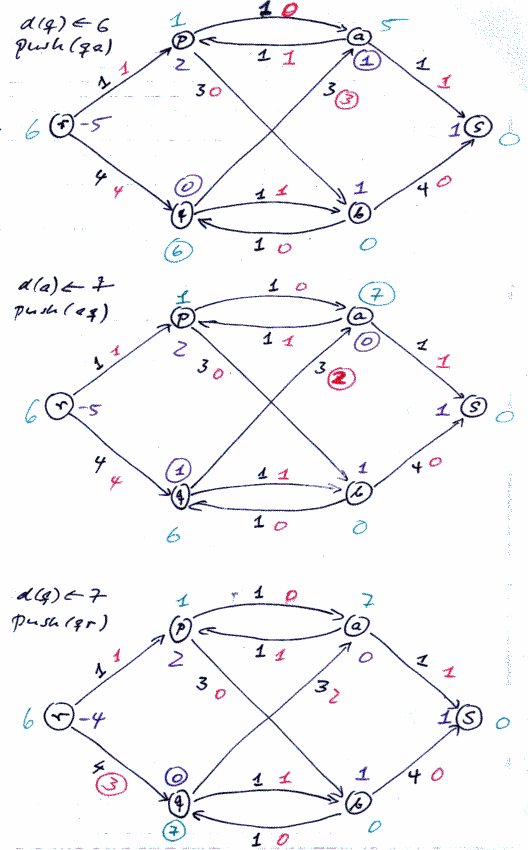
\includegraphics[width=5cm]{bilder/3-0Tarjan4}&
%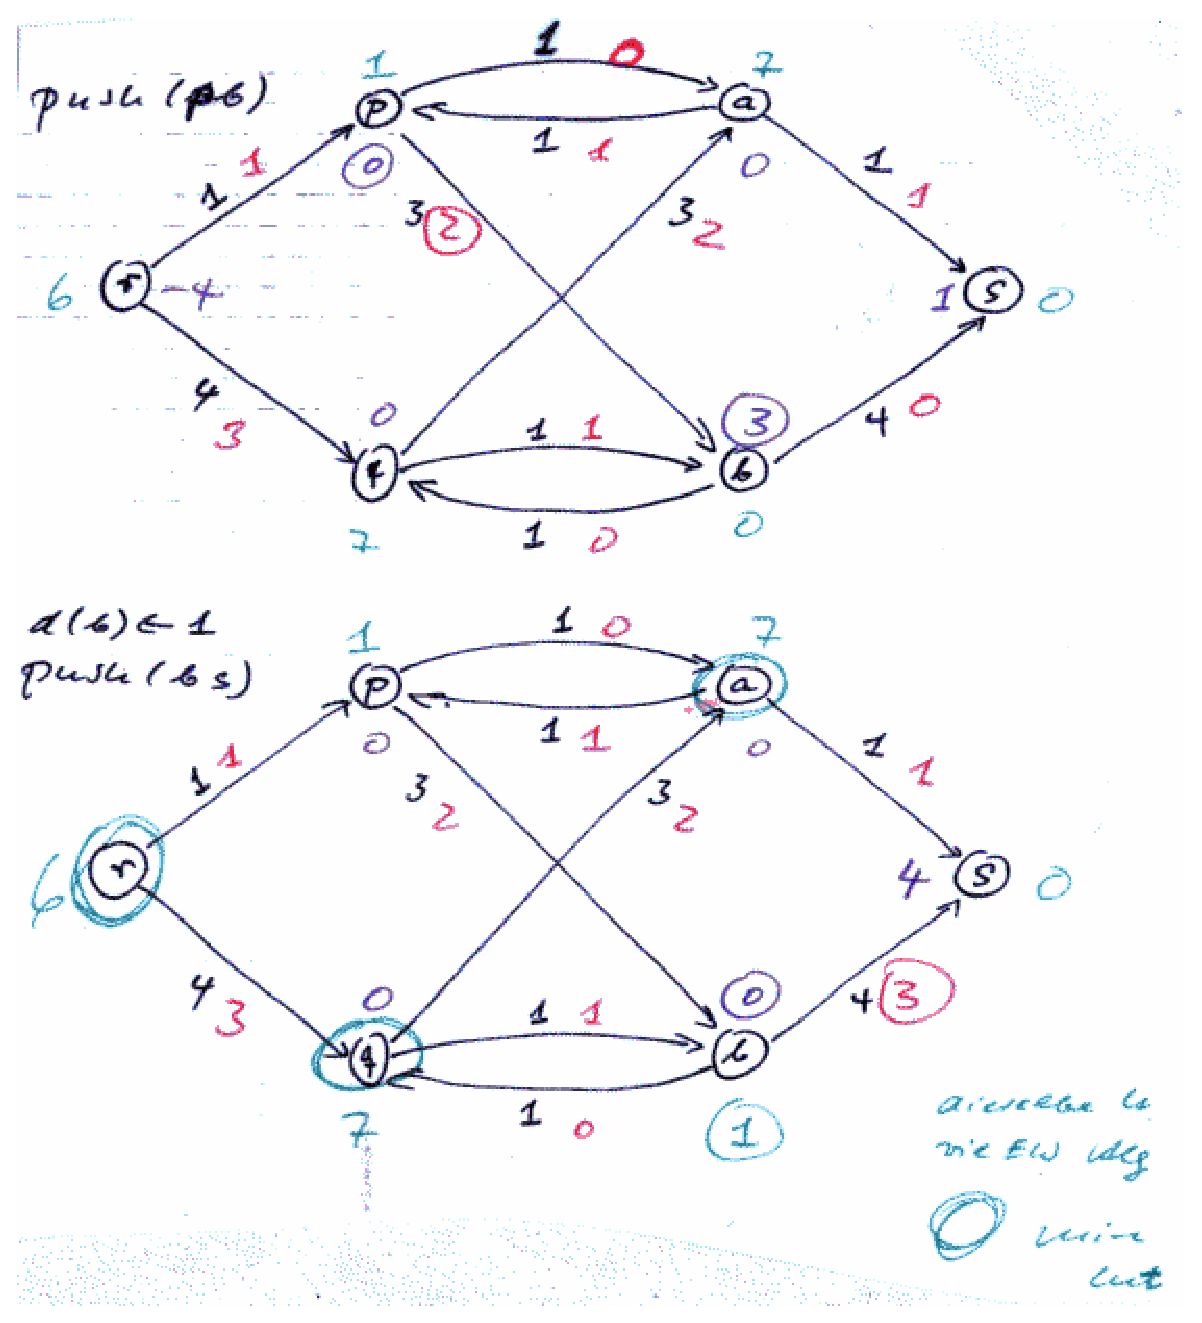
\includegraphics[width=5cm]{bilder/3-0Tarjan5}\end{tabular}

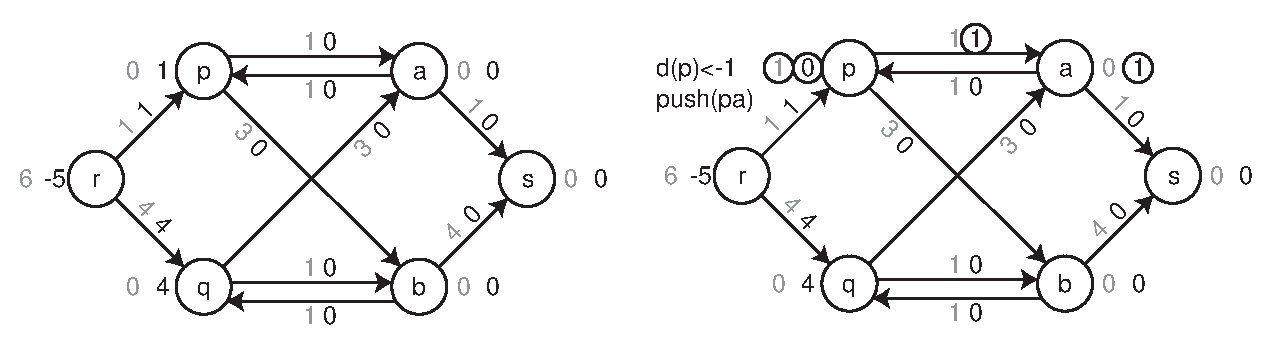
\includegraphics[width=15cm]{bilder/3-0GBTarjan1}

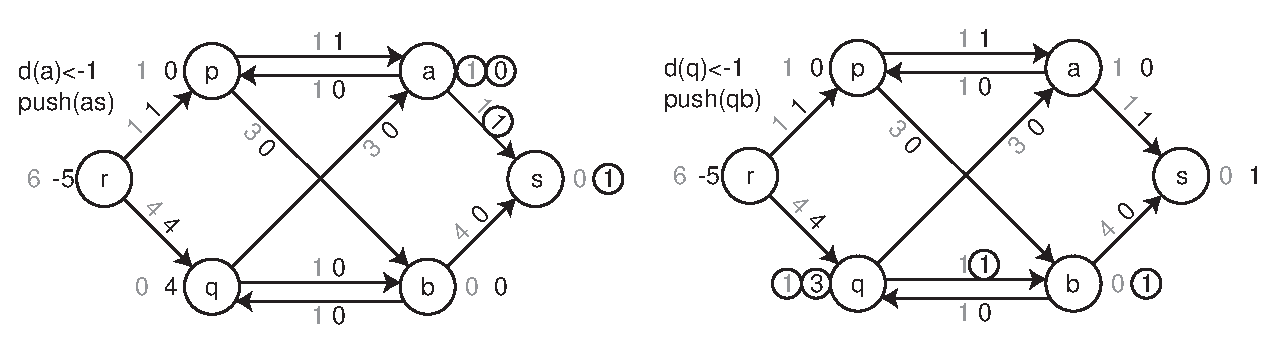
\includegraphics[width=15cm]{bilder/3-0GBTarjan2}

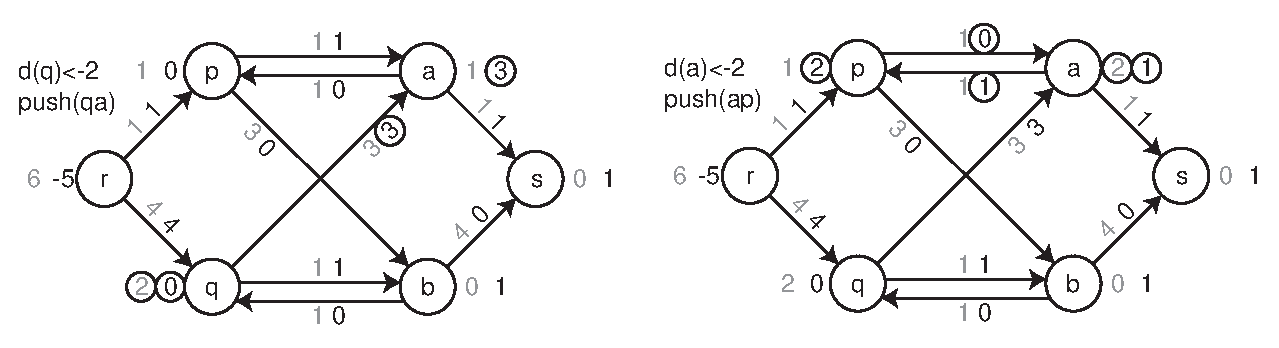
\includegraphics[width=15cm]{bilder/3-0GBTarjan3}

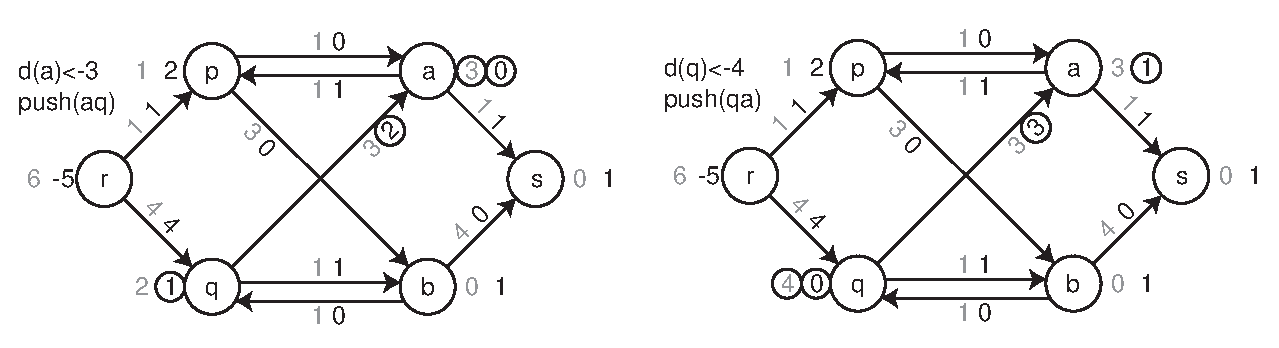
\includegraphics[width=15cm]{bilder/3-0GBTarjan4}

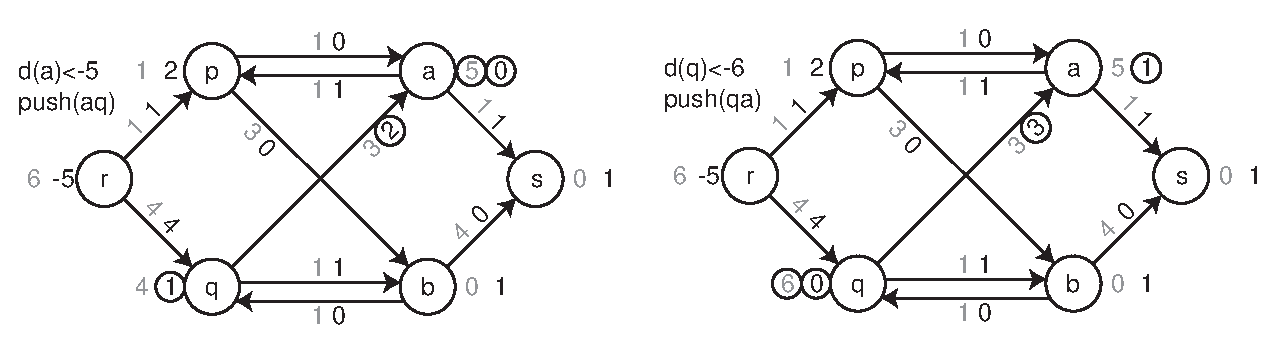
\includegraphics[width=15cm]{bilder/3-0GBTarjan5}

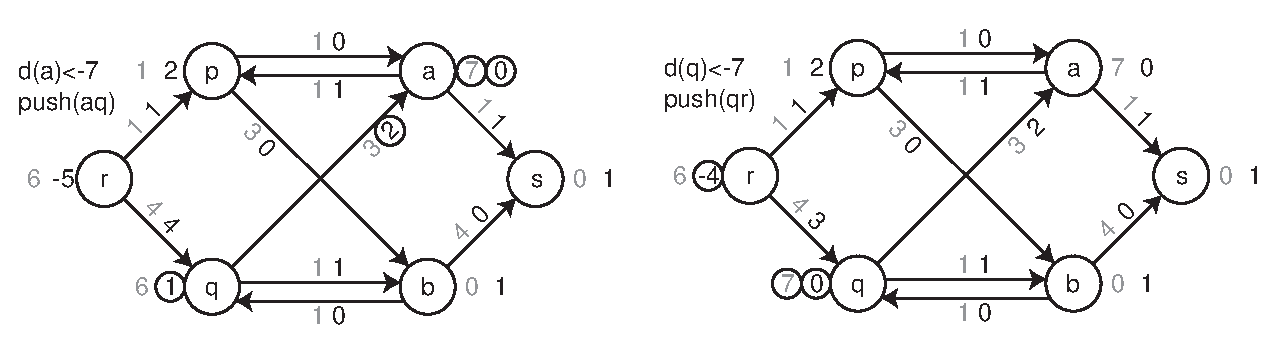
\includegraphics[width=15cm]{bilder/3-0GBTarjan6}

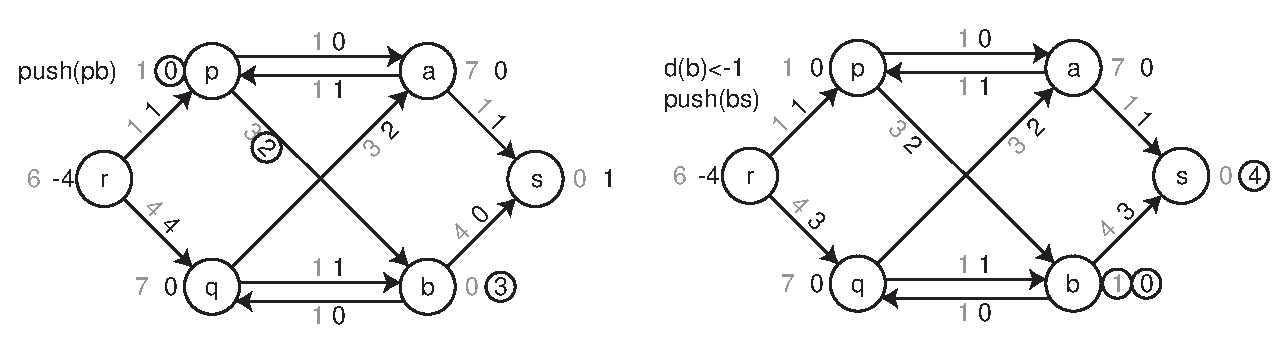
\includegraphics[width=15cm]{bilder/3-0GBTarjan7}


\begin{satz}
Der (max-distance) GT-Algorithmus ist korrekt. Der GT-Algorithmus führt
$O(n^{2})$ relabel Operationen durch, sowie $O(n^{2}m)$ push-Operationen in
der Urversion und $O(n^{2}\sqrt{m})$ in der max-dist-Version.

Die Urversion kann so implementiert werden, dass sie $O(n^{2}m)$ Zeit
benötigt, die max-dist-Version so, dass sie $O(n^{2}\sqrt{m})$ Zeit
benötigt.
\end{satz}
Beweis: Korrektheit folgt aus Korollar \ref{GueltmaxFluss}: Falls
GT-Algorithmus terminiert, so mit einem maximalen Fluss.

Die Laufzeit ist sehr aufwendig zu beweisen, deswegen verzichten wir an
dieser Stelle darauf.

Aus der Praxis kann man sagen das der GT-Algorithmus dort gute Ergebnisse
erzielt.

\section{Minimale Schnitte in ungerichteten Graphen ("`Min-Cut"')}

Gegeben: ungerichteter Graph $G=(V,E)$ mit Kantenkapazitäten $z_{e} \geqq 0
\; \; \forall \; e \in E$.

Gesucht: $\varnothing \neq S \subset V$ mit $z(\delta(S))$ Minimum.\\
Dieses Problem tritt z.B. als Teilproblem des TSP auf.

Spezialfall: $z_{e} = 1 \forall \; e \in E$: Bestimmung des
Knotenzusammenhangs. (minimale Anzahl von Kanten die entfernt werden müssen
um $G$ unzusammenhängend zu machen).

Sei $G$ zusammenhängend (sonst ist es trivial), z.B. Breitensuche findet in
Linearzeit ein $S$ mit $z(\delta(S))=0$. Das Problem kann
offensichtlich via ${n \choose 2}$ $(r,s)$-Max Flow-Min-Cut Berechnungen
gelöst werden. $\rightarrow$ Laufzeit $O(n^{5})$

\paragraph{Schrumpfen eines Knotenpaares $i,j \in V$} \mbox{} \\
\begin{enumerate}
\item $V \leftarrow V \wout \{ i,j\} \cup \{p\}\; \; \; $ $p$ ist also 
neuer Knoten.
\item Ersetze in $p$ jedes Paar von Kanten
\[e'=i k \hspace{5mm} e''= j k\]
durch:
\[e^{\ast} = p k \mbox{ mit } z_{e}^{\ast} = z_{e'} + z_{e''}\]
\item Ersetze in $E$ alle Kanten $i e$ durch $p e$ mit $z_{p e} = z_{i e}$
\item Ersetze in $E$ alle Kanten $je$ durch $p e$ mit $z_{p e} = z_{je}$
\end{enumerate}
Beispiel:

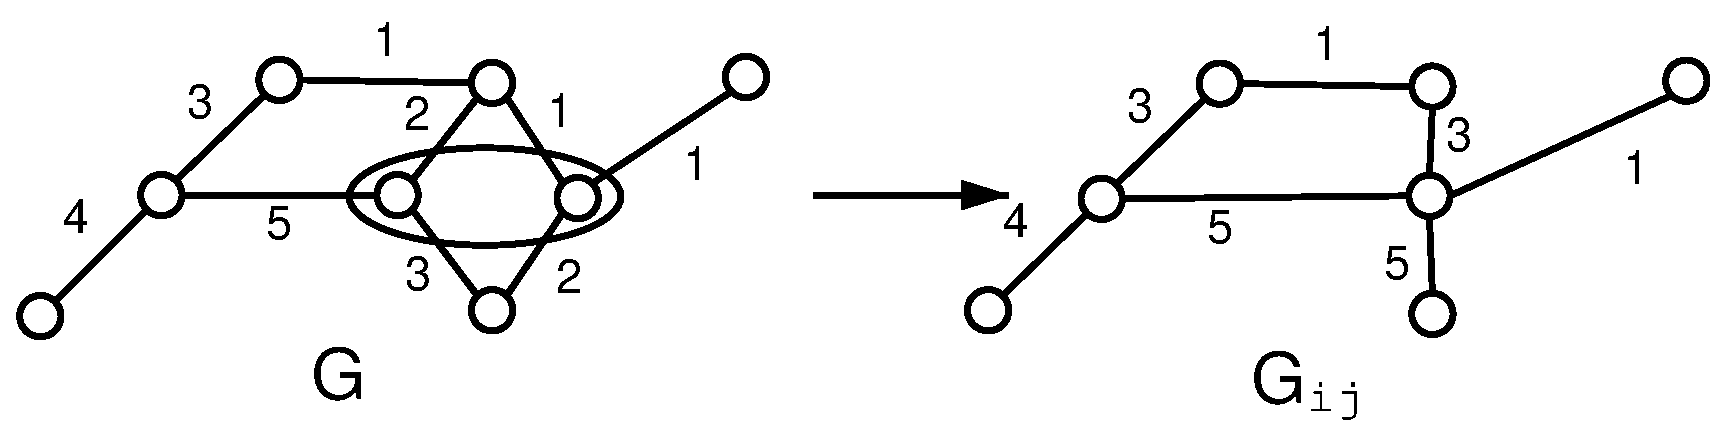
\includegraphics[height=3cm]{bilder/3-0KnotenSchrumpf}

$\lambda(G)$: Kapazität eines minimum Schnittes in $G$\\
$\lambda(G;i,j)$: Kapazität eines minimum i-j Schnittes in $G$

\begin{lemma}
$\lambda(G) = \min(\lambda(G_{i j}), \; \lambda(G;i,j))$
\end{lemma}

Beweis: trivial

\paragraph{Das Verfahren} \mbox{}\\
{
\renewcommand{\labelitemi}{\mbox{}}
\renewcommand{\labelitemii}{\mbox{}}
\renewcommand{\labelitemiii}{\mbox{}}
\renewcommand{\labelitemiv}{\mbox{}}
\begin{itemize}
\item $z^{\ast} := \infty$;
\item wiederhole $n-1$ mal:
\begin{itemize}
\item wähle $r,s \in V$;
\item Bestimme $(r,s)$-min-cut $\delta(S)$;
\item Falls $z(\delta(s)) < z^{\ast}$
\begin{itemize}
\item $S^{\ast} := S$;
\item $z^{\ast} := z(\delta(S))$;
\end{itemize}
\item Schrumpfe $r$ und $s$
\end{itemize}
\end{itemize}
}
liefert (mit G-T Algorithmus) eine Lösung in $O(n^{4})$ Zeit.

\subsubsection{Ein einfacher Min-Cut Algorithmus}

Grundidee: Nagamochi und Iberaki [1992]\\
Effiziente Implementierung von Nagamochi, Ono und Iberaki [1993]\\
einfache Korrektheitsbeweise: Frank [1994], Stoer u. Wagner [1994]\\
Beschreibung von Stoer und Wagner:\\
Notation $z(A:B)$: $\displaystyle \sum_{\begin{array}{c}a \in A\\b \in B
\end{array}} z_{ab} \; \; \mbox{ für } A, B \subseteq V$\\
$z(A:b)$ statt $z(A,\{b\})$

Erinnerung: Prims Algorithmus für einen minimum spannenden Baum: Min
Spanning Tree (G,z,a) [$a\in V$ beliebig].

\begin{algorithmic}
\STATE $W := \{a\}$;
\STATE $T := \varnothing$;
\WHILE{$W \not=V$}
\STATE wähle $v \not\in W$ mit $z_{w v} = \min \{z_{w v} | w \in W, w v \in
E\}$
\STATE $W := W \cup \{v\}$; \hspace{3mm} (Füge einen am schwächsten mit W
verbundenen Knoten hinzu)
\STATE $T := T \cup \{u v\}$;
\ENDWHILE
\end{algorithmic}
ähnlich:\\
{\bf Min\_Cut\_Phase}
\begin{algorithmic}
\STATE $W:= \{a\}$;
\WHILE{$W \neq V$}
\STATE wähle $v\not\in W $ mit $z(W:v) = \max\{z(W:v)|v \not\in W\}$;
\STATE $W:= W \cup \{v\}$; \hspace{3mm}(Füge einen am stärksten mit $W$ 
verb. Knoten hinzu)
\ENDWHILE
\STATE Sei $s$ der vorletzte, $t$ der vorletzte zu $W$ hinzugefügte Knoten.
\STATE $z^{\ast} := z(\delta(t))$;
\STATE $\delta^{\ast} :=$ Menge der von $t$ repräsentierten Orginalknoten
(Phasenschnitt);
\STATE Schrumpfe $s$ und $t$
\end{algorithmic}

{\bf Berechnung des Min-Cut($g,z,a$);}
\begin{algorithmic}
\STATE $z_{\min} := \infty$;
\WHILE{$|V| > 1$}
\STATE Min\_Cut\_Phase($G,z,a$);
\IF{$z^{\ast} < z_{\min}$}
\STATE $z_{\min} := z^{\ast}$;
\STATE $\delta_{\min} := \delta^{\ast}$;
\ENDIF
\ENDWHILE
\end{algorithmic}

\begin{lemma}
Jeder Phasenschnitt ist ein minimum $(s,t)$-Schnitt im jeweiligen
"`Phasengraphen"', wobei $s$ vorletzter und $t$ letzter zu $W$
hinzugefügter Knoten ist.
\end{lemma}

Beweis:\\
Situation: $\begin{array}{c}\stackrel{\mbox{\scriptsize
Hinzufügungsreihenfolge}}{\Longrightarrow}\\a \rightarrow \bullet \rightarrow 
\ldots \rightarrow s \rightarrow t\end{array}$\\
Sei $C \subseteq E$ ein beliebiger$(s,t)$-Schnitt in $G$\\
Wir zeigen $z(C) \geqq z^{\ast}=z(\delta(t))$\\
$v\neq a$ heißt {\it aktiv} bezüglich $C$, falls $w v \in C$ mit
$w=$ direkter Vorgänger von $v$.\\
$A_{v} \subseteq V$: Menge aller Vorgänger von $v$ (ohne $v$)\\
$C_{v} := \left\{x y \in C | x,y \in A_{v} \cup \{v\}\right\} \subseteq C$

Beispiel:

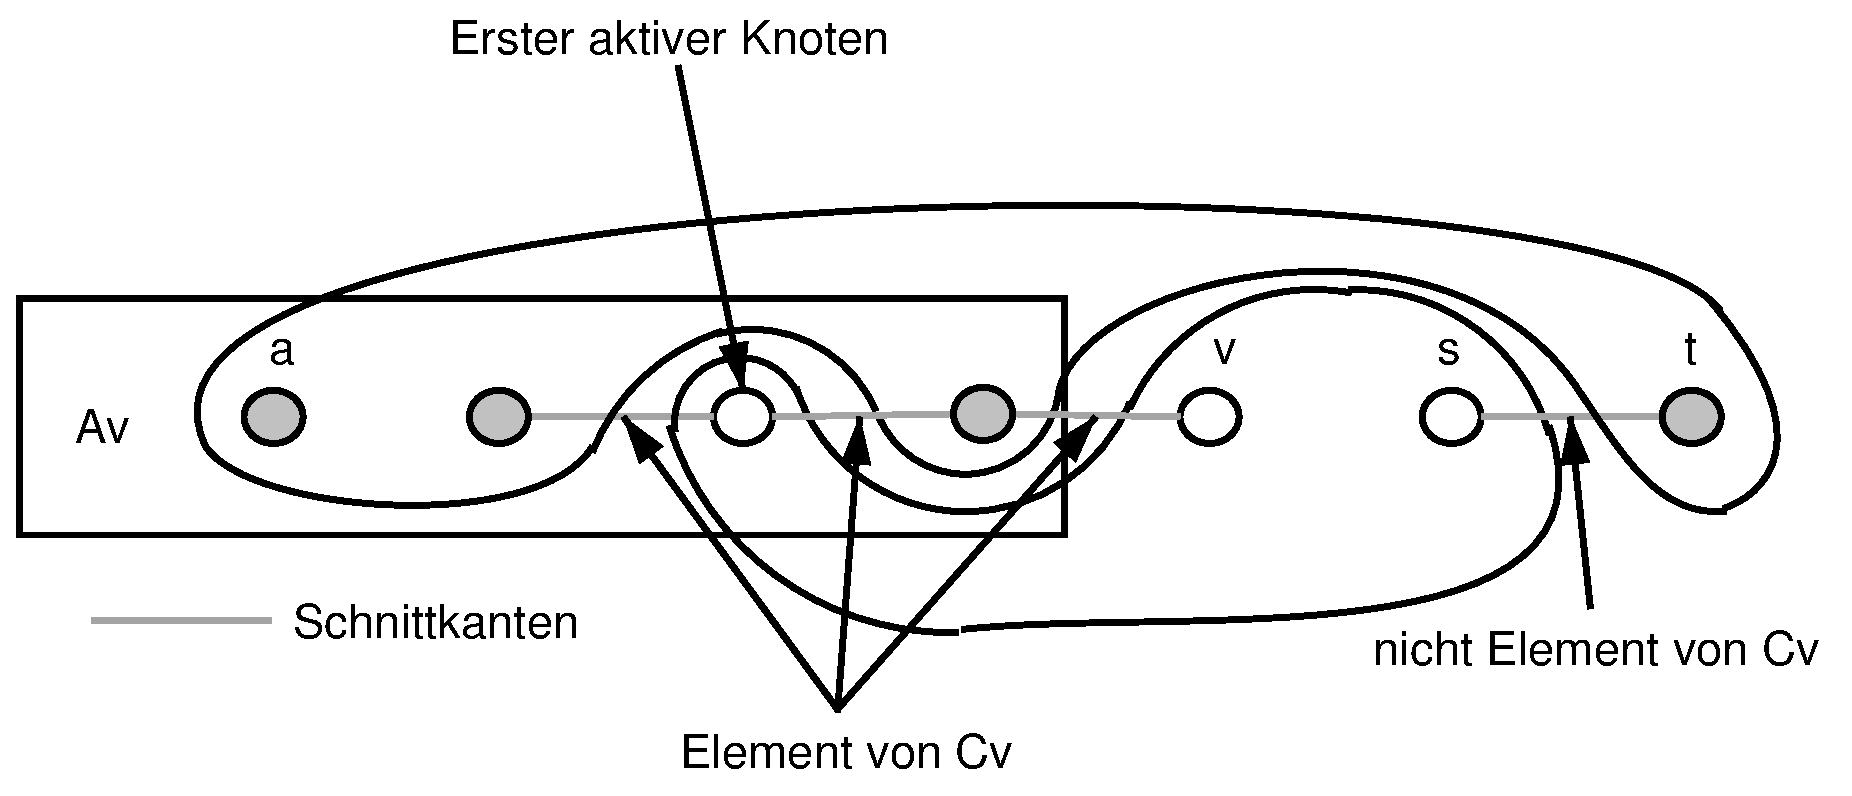
\includegraphics[width=12cm]{bilder/3-0Phasenschnitt1}

Behauptung: Für jeden aktiven Knoten gilt $z(A_{v}:v) \leqq z(C_{v})$.
Beweis: Induktion über aktive Knoten:\\
Für den ersten aktiven Knoten $v_{1}$ gilt $z(A_{v_{1}}:v_{1}) =
z(C_{v_{1}})$. Die Behauptung gelte für alle aktiven Knoten bis zu $v$. Sei
$n$ der nächste aktive Knoten.

Situation:\\
\[\underbrace{\underbrace{a \bullet\ldots \bullet}_{A_{v}\bullet}
\stackrel{\in C}{-} \underbrace{v\circ \ldots \circ}_{A_{u} \wout
A_{v}}}_{A_{u}}
\stackrel{\in C}{-}u \ldots s \ldots  t\]

Es gilt: $\begin{array}{rcl}z(A_{u}:u) &=& z(A_{v}:u) + z(A_{u} \wout A_{v} : 
u)\\
&\leqq& z(A_{v}:v) \hspace{5mm} (\mbox{Da $v$ stärkster mit $A_{v}$ verb.
Knoten})\\
&\leqq& z (C_{v})\\
&\leqq& z (C_{v}) + z ( A_{u} \wout A_{v} : u)
\end{array}$

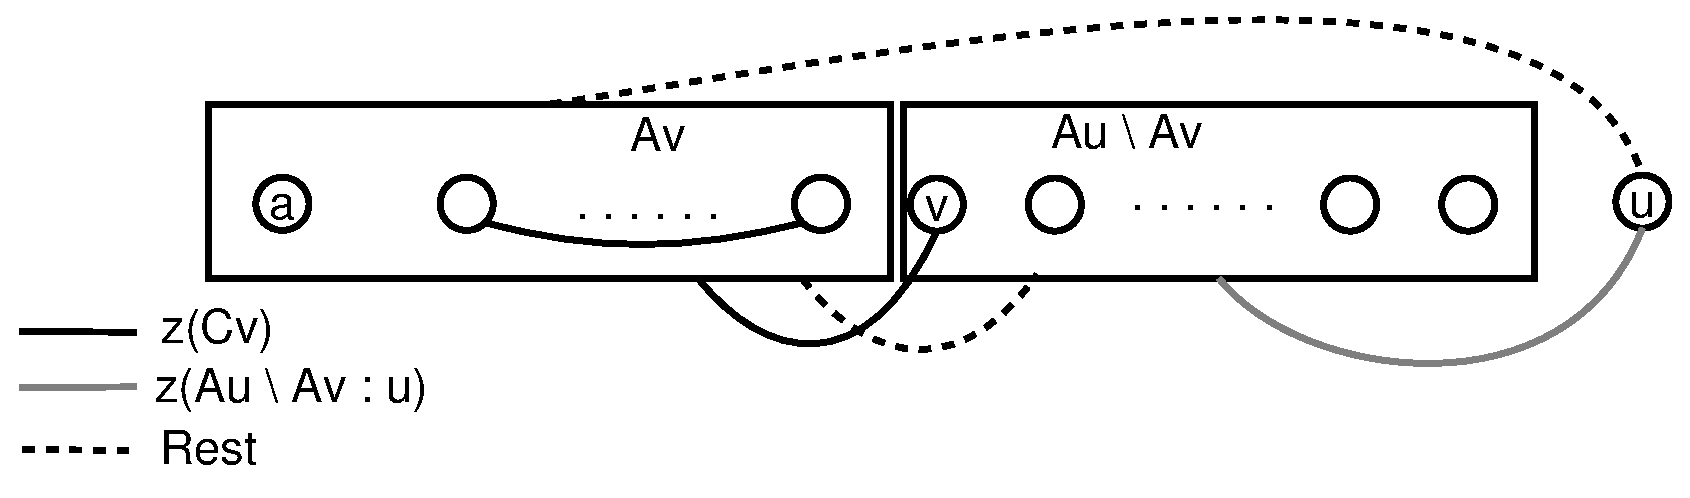
\includegraphics[width=12cm]{bilder/3-0Phasenschnitt2}

alles zusammen: $z(C_{u}) \leqq z(C_{u})$ q.e.d (Beh.)\\
$s t \in C \Rightarrow t \mbox{ aktiv } \Rightarrow  z^{\ast} = z(\delta(t))
= z(A_{t}:t) \leqq z(C_{t}) = z(C)$ q.e.d. (Lemma)

\paragraph{Laufzeit} \mbox{}\\
MINIMUM\_CUT\_PHASE\\
Prioritätsschlange für Knoten in $V\wout \{a\}$\\
\mbox{} \hspace{3mm}Schlüssel für $v \in V \wout \{a\}$\\
\mbox{} \hspace{6mm} key$(v) = z(W:v)$: Gesamtkapazität der Kanten zwischen
$v$ und derzeitigem $W$.
Neu hinzuzufügender Knoten $v$ via EXTRACT\_MAX\\
Update: key$(u) := key(u) + z_{v u}$ für $u \not \in W$ falls $v u \in E
\rightarrow$ INCREASE\_KEY\_OPERATION für jede Kante $e \in E$ genau einmal

insgesamt:\\
$\left. \begin{array}{rcll} n&=& |V| &\mbox{ EXTRACT\_MAX}\\
m&=& |E| &\mbox{ INCREASE\_KEY}\end{array} \right\}$ Operationen\\
mit Binär-Heaps (Informatik I) je:
$\left. \begin{array}{l} O(\log n)\\O(\log n)\end{array}\right\}$ Zeit\\
mit Fibonacci-Heaps je
$\left. \begin{array}{l}O(\log n)\\O(1)\end{array}\right\}$ Zeit

d.h. $O(m+n \log n)$ Zeit für MIN\_CUT\_PHASE\\
$O(n)$-Phasen $\rightarrow  O(m n + n^{2}\log n)$ Gesamtzeit.

\begin{satz}
Der Phasenschnitt-Algorithmus findet einen minimum Schnitt in einem
ungerichteten Graphen in $O(n m+n^{2}\log n)$ Zeit.
\end{satz}

In dieser Vorlesung teilte Prof. Jünger noch ein Blatt mit Beispielen zum
Phasenschnittalgorithmus sowie einen Artikel (Jünger M.; Rinaldi G.;
Thienel S. (2000). {\it Practical performance of efficient minimum cut
algorithms}. Algorithmica v26n1 S. 172-195).


}

\chapter{Minimale Kostenfl�sse}

{
\section{Optimalit�tsbedingungen, Reduktionen}

%\newcommand{\bc}{\bar{c}}

\[\begin{array}{rcl}
(\mbox{LPMKFP}) \hspace{7mm} \min \displaystyle \sum_{e \in E} c_{e} x_{e}\\
f_{x}(v) & = & b_{v} \; \; \; \forall \; v \in V\\
0 \leqq x_{e} &\leqq& u_{e} \; \; \; \forall e \in E
\end{array}\]
Man kann es auch ganzzahlig betrachten, dann gilt $x_{e} \in \ZZ$. 

$u \in (\RR \cup \{\infty\})^{E} \hspace{3mm} b(V) = 0 \hspace{3mm}
\begin{array}[t]{rcll}b_{v} &>& 0 & \mbox{Nachfrage an Knoten $v$}\\
b_{v} &<& 0 & \mbox{Vorrat}\end{array}$

Spezialf�lle:
\begin{itemize}
\item $c=0$: Zul�ssigkeitsproblem (L�sbar als Max-Fluss Problem)
\item $r,s \in V, \; b_{r}=-1, \; b_{s} = 1, \; b_{v} = 0 \; \forall \; v
\in V \wout \{r,s\}$, $ u_{e} = \infty \; \forall \; e \in E$ $\rightarrow$
dann ist es das LPKW
\item Transportproblem:\begin{itemize}
\item $G$ bipartit $V = P \cup Q$ (Bipartition)
\item $a_{p}$ $(p \in P)$ Vorrat
\item $b_{q}$ $(q \in Q)$ Nachfrage
\item $c_{p q}$ $(p q \in E)$  Transportkosten
\end{itemize}
\[\begin{array}{rcl}
\min \displaystyle \sum_{p q \in E} c_{p q} x_{p q}\\
\displaystyle \sum_{p q \in E} x_{p q} &=& b_{q} \; \; \forall \; q \in Q\\
\displaystyle \sum_{p q \in E} x_{p q} &=& a_{p} \; \; \forall p \in P
\mbox{ ( $\cdot -1$ macht daraus ein LPMKFP)}\\
x_{p q} &\geqq& 0 \; \; \forall p q \in E
\end{array}
\]
wenn zus�tzlich $x_{p q} \leqq u_{p q}$ gilt handelt es sich um ein
kapazitiertes Transportproblem.
\item $u_{e} = \infty \; \forall e \in E$: Transshipment Problem
\end{itemize}

Dualisieren:
\[\begin{array}{rcl@{\hspace{6mm}}l}
(\mbox{LPMKFP}) \hspace{7mm} \min \displaystyle \sum_{e \in E} c_{e}
x_{e}\\
f_{x}(v) & = & b_{v} \; \; \; \forall \; v \in V& (y)\\
- x_{v w} &\geqq& - u_{v w} \; \; \forall \; v w \in E& (z)\\
x_{v w} &\geqq& 0 \; \; \forall \; v w \in E
\end{array}\]

\[\begin{array}{rcl}
(\mbox{DLPMKFP}) \hspace{7mm} \max \displaystyle \sum_{v\in V} b_{v}y_{v} -
\sum_{v w \in E} u_{v w} z_{v w}\\
- y_{v} + y_{w} - z_{v w} &\leqq& c_{v w} \; \; \forall \; v w \in E\\
z_{v w} &\geqq& 0 \; \; \forall \; v w \in E
\end{array}\]
falls $u_{v w} = \infty \rightarrow$ keine Variable $z_{v w}$

$\bar{c}_{v w} := c_{v w} + y_{v} - y_{w}$ "`reduzierte Kosten von $v w$"'\\
$u_{e} = \infty \Rightarrow \bar{c}_{e} \geqq 0$\\
$u_{e} \neq \infty \Rightarrow z_{e} \geqq - \bar{c}_{e}$, $z_{e} \geqq 0$\\
Setze $z_{e} = \max\{0, -\bar{c}_{e}\}$ d.h. $z_{e}$ "`unn�tig"'

Beschr�nkung auf $y$:\\
Komplement�re Schlupfbedingungen\\
$\begin{array}{rcl} x_{e} > 0 &\Rightarrow& -\bar{c}_{e} = z_{e} = \max\{0,
- \bar{c}_{e}\}\\
&\Leftrightarrow& \bar{c}_{e} \leqq 0\end{array}$\\
$z_{e} > 0 \Rightarrow -\bar{c}_e>0 \Rightarrow \bar{c}<0 \Rightarrow 
x_{e} = u_{e}$\\
$\Leftrightarrow -\bar{c}_{e} > 0 \Leftrightarrow c_{e} < 0$

\begin{satz} \label{ZulLLPMKFP}
Eine zul�ssige L�sung $x$ von (LPMKFP) ist optimal genau dann wenn ein $y
\in \RR^{V}$ existiert, so dass f�r alle $e \in E$ gilt:
\[\begin{array}{rcl}
\bar{c}_{e} < 0 &\Rightarrow& x_{e} = u_{e} \hspace{5mm} (\neq \infty)\\
\bar{c}_{e} > 0 &\Rightarrow& x_{e} = 0
\end{array}\]
\end{satz}

Kosten eines Weges $P$ $\bullet\rightarrow\bullet\rightarrow\bullet
\rightarrow\ldots \rightarrow\bullet\rightarrow\bullet$:
\[C_{p} = \sum_e \in P, \; e \mbox{ vorw�rts } c_{e} -  \sum_e \in P, \; e
\mbox{ r�ckw�rts } c_{e}\]
Ein $x$-erh�hender Weg $P$ mit Erh�hung um $\epsilon$, entspricht einer
Kosten�nderung 
\[c^{T}x \rightarrow c^{T}x + \epsilon C_{P}\]
Verbesserung eines zul�ssigen $x$-erh�henden Kreises mit negativen
Kosten mit einem Hilfsdigraph G(x):\\
$\forall vw \in E$ mit $x_{vw} < u_{vw}$ Kosten $c'_{vw} = c_{vw}$\\
$\forall vw \in E$ mit $x_{vw} > 0 $ Kosten $c'_{wv} = - c_{vw}$\\
Beispiel (c,u,x):

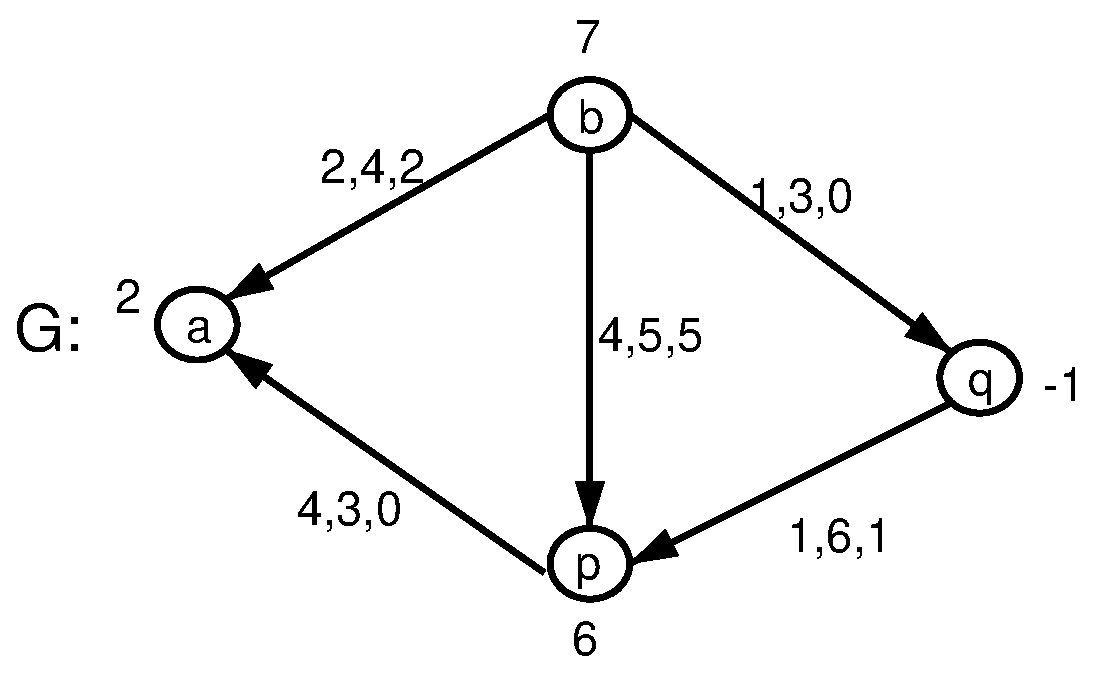
\includegraphics[width=6cm]{bilder/4-1Hilfsdigr1} \hspace{1cm} 
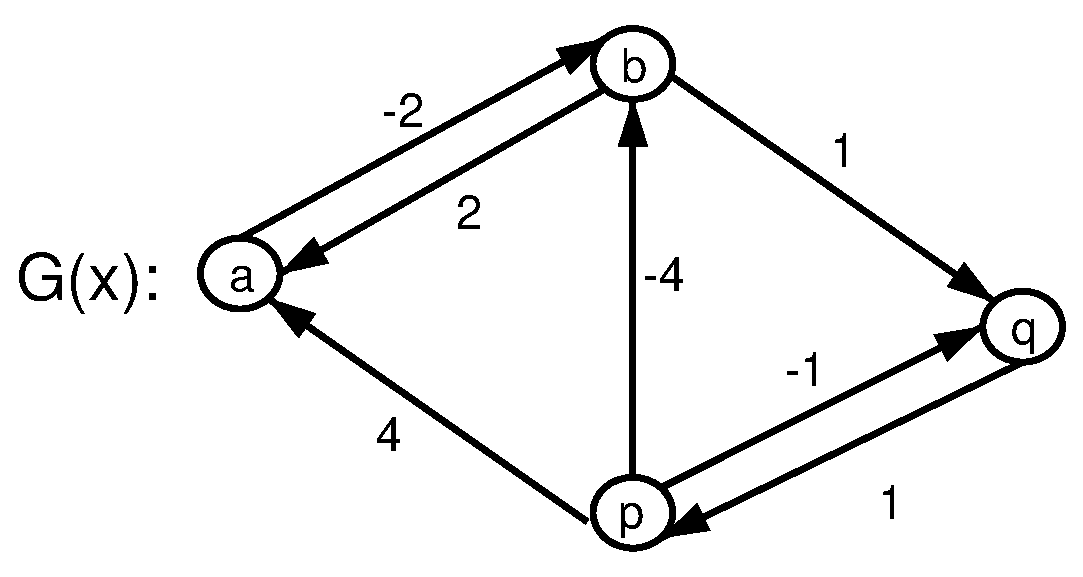
\includegraphics[width=6cm]{bilder/4-1Hilfsdigr2}

z.B. negativen Kreis $p b q$ um 3 erh�hen (Kostenminderung um 6):

\includegraphics[width=6cm]{bilder/4-1Hilfsdigr3}

\begin{satz} \label{L�sungLPMKFPopt}
Eine Zul�ssige L�sung $x$ von (LPMKFP) ist optimal g.d.w. kein
$x$-erh�hender Kreis mit neg. kosten existiert.
\end{satz}

Beweis:

\includegraphics[width=7cm]{bilder/4-1BeweisSatz42}


L�se das k�rzeste Wege Problem in $G'$.\\
Resultat: Entweder negativer Kreis oder zul�ssiges Potential:
\begin{enumerate}
\item M�glichkeit: Negativer Kreis: enth�lt $r$ nicht, liefert also
$x$-erh�henden Kreis mit negativen Kosten.
\item M�glichkeit: zul. Potential:
\[\begin{array}{ll}
&y_{v} + c'_{v w} \geqq y_{w} \; \forall \; v w \in E(G(x))\\
\Leftrightarrow&\left\{\begin{array}{l}
y_{v} + c_{v w} \geqq y_{w} \mbox{ falls }x_{v w} < u_{v w}\\
y_{v} - c_{w v} \geqq y_{w} \mbox{ falls }x_{w v} > 0 \end{array} \right\}\\
\Leftrightarrow&\left\{\begin{array}{l}
x_{e} < u_{e} \Rightarrow \bar{c}_{e} \geqq 0\\
x_{e} > 0 \Rightarrow \bar{c}_{e} \leqq 0\end{array} \right\}
\mbox{\begin{tabular}{l}"`Konstruktion eines optimalen $y$\\ 
aus einem optimalen $x$"'\end{tabular}}\\
\Leftrightarrow & \left\{\begin{array}{l} \bar{c}_{e} < 0 \Rightarrow x_{e}
= u_{e}\\
\bar{c}_{e} > 0 \Rightarrow x_{e} = 0 \end{array} \right\} \hspace{2mm}
\mbox{Optimalit�tsbed. aus Satz \ref{ZulLLPMKFP} q.e.d. }
\end{array}\]
\end{enumerate}

\begin{satz}
Hat (LPMKFP) eine Optimall�sung und ist ganzzahlig, so kann $y$ in Satz
\ref{ZulLLPMKFP} ganzzahlig gew�hlt werden, d.h. (DLPMKFP) hat eine
ganzzahlige Optimall�sung.
\end{satz}
Beweis:
Kantengewichte ganzzahlig $\Rightarrow$ K�rzeste Wege Kosten ganzzahlig
q.e.d.
\begin{satz} \label{L�sungLPMKFPopt3}
hat (LPMKFP) eine zul�ssige L�sung so existiert eine Optimall�sung genau
dann, wenn es keinen negativ gerichteten Kreis gibt, dessen Kapazit�ten
alle unbeschr�nkt sind.
\end{satz}
Beweis:\\
"`$\Rightarrow$"' $\exists$ negativer Kreis$\ldots$ $\Rightarrow$ (LPMKFP)
unbeschr�nkt. trivial.\\
"`$\Leftarrow$'" $\nexists$ negativer gerichteter Kreis ...\\
Es reicht zu zeigen (DLPMKFP) hat zul�ssige L�sung $(y,z)$\\
F�r $u_{e} \neq \infty$ w�hle $z_{e} = \max\{0,-c_{e}\}$\\
Also brauchen wir $y$ mit $\bar{c}_{e} \geqq 0 \; \; \forall e$ mit $u_{e} =
\infty$

\includegraphics[width=8cm]{bilder/4-1BeweisSatz44}

w�hle $y$ als zul�ssiges Potential in $G'$. q.e.d.

\paragraph{Konstruktion eines optimalen $x$ aus optimalem $y$} \mbox{}\\
Bedingungen f�r $x$:
\[(\ast)\left\{\begin{array}{l}
f_{x}(v) = b_{v} \; \; \forall \; v \in V\\
0 \leqq x \leqq u\\
\bar{c}_{e} > 0 \Rightarrow x_{e} = 0\\
\bar{c}_{e} < 0 \Rightarrow x_{e} = u_{e}
\end{array} \right.
\]
Definiere:
\[\begin{array}{rl}
u'_{e} = & \left\{ \begin{array}{l} 0 \mbox{ falls }\bar{c}_e > 0\\
u_{e} \mbox{ sonst}\end{array}\right.\\
l'_{e} = & \left\{ \begin{array}{l} u_{e} \mbox{ falls } \bar{c}_{e} < 0\\
0 \mbox{ sonst}\end{array}\right.\\
(\ast) \Leftrightarrow (\ast\ast)& \left\{ \begin{array}{l} f_{x}(v) =
b_{v}\\ l' \leqq x \leqq u'\end{array} \right.
\end{array}\]
L�se $(\ast\ast)$ mittels Maximum-Fluss-Algorithmus.

\begin{satz}
Sind $b$ und $u$ ganzzahlig und hat (LPMKFP) eine Optimall�sung, so
existiert eine ganzzahlige Optimall�sung. q.e.d.
\end{satz}

Reduktionen:
\begin{description}
\item[A] \[\begin{array}{rcll} \min c^{T}x\\
a_{v}\leqq f_{v}(x) &\leqq& b_{v} &\; \; \forall \; v \in V\\
l_{e} \leqq x_{e} &\leqq& u_{e} & \; \; \forall e \in E \end{array} \]
auf (MKFP)\\
Wir d�rfen annehmen, dass
\item[A1] $(\forall \; v \in V) \; \; a_{v} = b_{v} $

\begin{tabular}{cc}\includegraphics[width=8cm]{bilder/4-1Reduktion1}&
$\begin{array}[b]{lcl}
c_{r v} &=&0\\
l_{r v} &=& 0\\
u_{r v} &=& b_{v}- a_{v}\\
b_{r}&=& \displaystyle - \sum_{v \in V} b_{v}\\
\multicolumn{3}{l}{\mbox{Ersetze alle $a_{v}$ durch $b_{v}$}}
\end{array}$
\end{tabular}

im neuen Problem gilt:
\[\begin{array}{l}x_{r v} + f_{x}(v) = b_{r} \; \; \forall r \in V\\
\Rightarrow x_{r v} = b_{v} -f_{x}(v)\end{array}\]
D.h.:\\
\[\begin{array}{l}a_{v} \leqq f_{x}(v) \leqq b_{v} \Leftrightarrow 0 \leqq x_{r v} \leqq b_{v} -
a_{v}\\
\Leftrightarrow a_{v} \leqq b_{v} - \underbrace{x_{r v}}_{\geqq 0}
\underbrace{\leqq}_{\mbox{redundant}} l_{v}\\
\Leftrightarrow x_{r v} \leqq b_{v} - a_{v}
\end{array}\]
Zul�ssige L�sungen des neuen Problems eingeschr�nkt auf die alten Kanten
sind genau die zul�ssigen L�sungen des alten Problems:
\begin{itemize}
\item Gleicher ZF-Wert
\item $O(m)$ Kanten $O(n)$ Knoten, d.h. keinen Effizienzverlust
\end{itemize}
\item[A2] $(\forall \; e \in E) \; l_{e} \neq -\infty$ oder $u_{e} \neq
\infty$\\ Dies wird eine �bungsaufgabe sein!
\item[A3] $(\forall \; e \in E)\;  l_{e} \neq \infty$\\
Nach A2 gilt: $l_{e} = -\infty \Rightarrow u_{e} \neq \infty$\\
Ersetze $v\stackrel{e}{\rightarrow}w$ durch $v\stackrel{e'}{\leftarrow}w$
\[\begin{array}{lcl}
c_{e'}&=& -c_{e}\\
l_{e'} &=& -u_{e}\\
u_{e'} &=& \infty
\end{array}\]
\item[A4] $(\forall \; e \in E)\; l_{e} = 0$\\
$u_{e} := u_{e} - l_{e}$\\
$\begin{array}{rcl}(e=vw) \; b_{v} &:=& b_{v} + l_{e}\\
b_{w} &=& b_{w} - l_{e} \end{array}$\\
$l_{e} := 0$

\begin{tabular}{llc}
vorher:&$\overbrace{v}^{b_{v}}\stackrel{l_{e}\leqq x_{e} \leqq
u_{e}}{\longrightarrow}\overbrace{b_{w}}^{b_{w}}$& Fluss mit Kosten $k$\\
nachher:&$\overbrace{v}^{b_{v}+l_{e}}{v}\stackrel{0\leqq x_{e} - l_{e} \leqq
u_{e} - l_{e}}{\longrightarrow}\overbrace{w}^{b_{w}-l_{e}}$& Fluss mit Kosten
$k - c_{e} l_{e}$\end{tabular}
\item[B] (MKFP) auf das Transshipment\\
$v\stackrel{c_{e}, \; u_{e} \neq \infty}{\longrightarrow} w \; \; \;
\rightarrow \;\; \; v
\stackrel{c_{e},\, \infty}{\longrightarrow}p\stackrel{0,\;
\infty}{\longleftarrow}q\stackrel{0,\, \infty}{\longrightarrow}w$ mit
$b_{p} = u_{e}$ und $b_{q} = -u_{e}$ \\
Vor der Umwandlung $O(m+n)$ Knoten und $O(m)$ Kanten. Nach der Umwandlung
$O(n+2m)$ Knoten und $O(3m)$ Kanten. Das ist in der Praxis ineffizient,
aber genug um zu zeigen, dass gewisse Algorithmen polynomiell sind.
\end{description}

\section{Primale Minimum Kosten Fluss Algorithmen}
\subsection{Basis-Algorithmus}
Dieser Algorithmus stammt von Kanorovich [1942]. Er l�uft so:\\
\begin{algorithmic}
\STATE Finde eine zul�ssige L�sung $x$;
\WHILE{($\exists$ $x$-erh�hender Kreis mit negativen Kosten)}
\STATE Finde einen $x$-erh�henden Kreis $C$ mit negativen Kosten;
\IF{($C$ hat keine R�ckw�rtskanten und keine Vorw�rtskanten mit endl.
Kapazit�t)}
\STATE STOP "`unbeschr�nkt"';
\ENDIF
\STATE Augmentiere $x$ auf $C$;
\ENDWHILE
\end{algorithmic} 

Dabei stellt sich die Frage, wie viele Flusserh�hungen durchgef�hrt
werden.\\
Max-Fluss-Problem als spezielles MKFP

\includegraphics[height=4cm]{bilder/4-2MaxFlussalsMKFP}

$x$-erh�hende Wege $\entspricht$ negative Kreise.\\
$\Rightarrow$ evtl. keine Terminierung.

\paragraph{Abhilfe} Max-Fluss: K�rzeste augmentierende Wege\\
hier: "`negativste"' Kreise?\\
nein: die Kreise im Beispiel sind "`negativst"', stattdessen:\\
minimale Durchschnittskosten f�r Kreis $C$
\[ := \frac{\mbox{Kosten }C}{\mbox{L�nge }C}\]
$\entspricht$ k�rzeste Wege im Max-Fluss.\\
Zeit pro Iteration $O(m n)$ mit Bellmann Ford $\leftarrow$ zu teuer\\
aber: ergibt polynomiellen Algorithmus (nach Goldberg u. Tarjan [1989])

\subsection{Die Netzwerk-Simplex Methode}

Erinnerung: Satz \ref{Spaltenb-Baum}: Spaltenbasen entsprechen eins zu eins
den aufspannenden B�umen.

Hier anderer Zugang: Spezialisierung des Basis-Algorithmus.
Annahme: $G$ ist zusammenh�ngend (OBdA: sonst Zusammenhangs-Komponenten 
getrennt behandeln)

$\rightarrow G$ hat aufspannenden Baum (ab jetzt genannt Baum)\\
Zun�chst Spezialisierung auf das Transshipment-Problem. ($u_{e} = \infty \;
\forall \; e \in E)$

Baum-L�sung $x \in \RR^{E}$ mit:
\[\begin{array}{rcll} f_{x}(v) &= &b_{v} &\; \; \forall v \in V\\
x_{e}&=&0 &\; \; \forall \; e \not\in T \end{array}\]
f�r einen Baum $T$

\begin{lemma}
Zu je zwei Knoten $u$ und $v$ eines Baumes $T$ existiert ein eineindeutiger
$(u,v)$-Weg in $T$. Beweis klar. q.e.d
\end{lemma}

\begin{lemma}
Ein Baum $T$ bestimmt eindeutig seine Bauml�sung.
\end{lemma}

Beweis:\\
$r \in V(T)$ beliebig fest "`Wurzel"'\\
$h=p q \in E(T)$\\
$R(T,h) = \{v \in V(T) | \mbox{eindeutiger $(r,v)$-Weg in T benutzt $h$
nicht}\}$

\includegraphics[height=4cm]{bilder/4-2BeweisL47}

$\Rightarrow x_{h} = \left\{\begin{array}{ll}-b(R(T,h)) \mbox{ falls } p
\in R(T,h)\\ b(R(T,h)) \mbox{ falls } q \in R(T,h)\end{array}\right.
\mbox{q.e.d.}$\\
Die Umkehrung gilt nicht, z.B. alle $b_{v} = 0 \Rightarrow$ alle
Bauml�sungen $\entspricht x=0$

\begin{satz}
Hat $(G,b)$ eine zul�ssige L�sung, so auch eine zul�ssige Bauml�sung, hat
$(G,b)$ eine optimale L�sung, so auch eine optimale Bauml�sung.
\end{satz}
Beweis: Sei $x$ eine zul�ssige L�sung, aber keine Bauml�sung\\
$\Rightarrow \exists$ Kreis $C$ mit positivem Fluss auf jeder Kante (OBdA
habe $C$ eine R�ckw�rtskante, sonst w�hle $C$ anders herum).

$\epsilon := \min \{x_{e} | e \mbox{ ist R�ckw�rtskante} \}$
$x_{e} \rightarrow \left\{ \begin{array}{ll} x_{e} + \epsilon \mbox{ falls $e$
Vorw�rtskante in $C$}\\
x_{e}-\epsilon  \mbox{ falls $e$ R�ckw�rtskante in $C$} \end{array}
\right.$

Resultat: Ein neues zul�ssiges $x$ mit weniger Kanten mit positivem Fluss\\
Schlie�lich: Bauml�sung

Jetzt $x$ optimale L�sung, Kreis $C$ mit positivem Fluss.\\
Aus Satz \ref{L�sungLPMKFPopt}: (zul�ssiges $x$ ist optimal g.d.w. kein
neg. Kreis)
$\Rightarrow C$ hat Kosten 0\\
Weiter wie oben 

\subsubsection{Grundidee der Netzwerk-Simplex-Methode}
\begin{itemize}
\item Erzeuge Eine Folge von Bauml�sungen
\item Suche nach speziellen negativen Kreisen zu jeder Kante $e=v w \not\in
T$ existiert ein eindeutiger Kreis C(T,e) mit:
\begin{itemize}
\item $f \in C(T,e) \rightarrow f \in T \cup \{e\}$
\item $e$ ist Vorw�rtskante in $C(T,e)$
\item Der "`Anfangsknoten"' $s$ von $C(T,e)$ ist der erste gemeinsame
Knoten der einfachen $(v,r)$- und $(w,r)$-Wege in $T$
\end{itemize}
\end{itemize}

\includegraphics[height=3cm]{bilder/4-2NetzSimpl1}

\begin{satz}\label{NSBaumopt}
Definiert der Baum $T$ die zul�ssige Bauml�sung und hat $C(T,e)$
nicht-negative Kosten f�r alle $e \not \in T$, so ist $x$ optimal.
\end{satz}
Beweis: Sei $y\in \RR^{V}$ mit $y_{v} =$ Kosten des einfachen $(r,v)$-Wege
in $T$. F�r alle $v,w \in V$ gilt: Kosten des einfachen $(v,w)$-Wege
$=y_{w} - y_{v}$.

\includegraphics[height=3cm]{bilder/4-2NetzSimpl2}

Also gilt f�r die reduzierten Kosten: $\bar{c}_{v w} = c_{v w } + y_{v} -
y_{w}$\\
falls $v w \in T$: $\bar{c}_{v w} = c_{v w} + y_{v} - y_{w} = y_{w} - y_{v}
+ y_{v}-y_{w} = 0$\\
$\mbox{falls }v w \in E \wout T: \; \bar{c}_{v w} \begin{array}[t]{l}= \underbrace{c_{v
w}}_{\mbox{\small Kosten $v w$}} + \underbrace{y_{v} -y_{w}}_{\mbox{\small Kosten im Baum
von $w$ nach $v$}}\\ =$ Kosten von $C(T, v w) \geqq 0\end{array}$
 
\includegraphics[height=3cm]{bilder/4-2NetzSimpl3}

D.h. die Bedingung von Satz \ref{ZulLLPMKFP} (Komplement�rer Schlupf
$\bar{c}_{e} > 0 \Rightarrow x_{e} = 0$) sind erf�llt.
$\stackrel{\mbox{\footnotesize Satz \ref{ZulLLPMKFP}}}{\Rightarrow}$ Optimalit�t.

Test ob $T$ diese Optimalit�tsbedingungen erf�llt:\\
$\left.\begin{array}{l}
\mbox{- Berechne $y$: Zeit $O(n)$}\\
\mbox{- Berechne $\bar{c}$: Zeit $O(m)$}\end{array} \right\}
\mbox{Besser als $O(m n)$ f�r Bellmann-Ford aber:}$\\
Problem: Verbessert $C(T,e)$ die L�sung?\\
$C(T,e)$ kann eine R�ckw�rtskante mit 0-Fluss haben.

\includegraphics[height=3cm]{bilder/4-2NetzSimpl4}

$C(T,w r)$ hat positive Kosten 1.\\
$C(T, v q)$ hat negative Kosten -2, aber R�ckw�rtskante $v w $ mit
0-Fluss.\\ Aber $x$ ist nicht optimal.\\
Eine Einheit Fluss auf dem durch die kurzen Pfeile markierten Kreis liefert
eine bessere L�sung (um -1).

Trotzdem:

\includegraphics[height=3cm]{bilder/4-2NetzSimpl5}


\subsubsection{Netzwerk-Simplex-Algorithmus f�r das 
Transshipment-Problem}

\begin{algorithmic}
\STATE Finde Baum $T$ mit zul�ssiger Bauml�sung $x$;
\STATE Berechne f�r alle $v\in V$ $y_{v} =$ Kosten des $(r,v)$-Weges in
$T$;
\WHILE{($\exists e = v w$ $(e\not\in T)$ mit $\bar{c}_{e} = c_e+ y_{v} - y_{w} < 0$)}
\STATE Finde solches $e$;
\IF{($C(T,e)$ hat keine R�ckw�rtskante)}
\STATE STOP unbeschr�nkt;
\ENDIF
\STATE Berechne $\Theta = \min\{x_{j} | j \mbox{ r�ckw�rts in } C(T,e)\}$
\STATE Bestimme R�ckw�rtskante $h$ von $C(T,e)$ mit $x_{h} = \Theta$;
\STATE Augmentiere $x$ um $\Theta$ auf $C(T,e)$;
\STATE Setze $T := (T \cup \{e\}) \wout \{h\}$;
\STATE Berechne neue $y$;
\ENDWHILE
\end{algorithmic}

Erzeugung eines ersten Baumes (Initialisierung):

\includegraphics[height=3.5cm]{bilder/4-2NetzSTrans}

K�nstliche Kanten, Hohe kosten $M$ falls $\not\in G$\\
$M := n\cdot \max\{|c_{e}|:\;  e \in E\} + 1$

\begin{lemma}\label{EntfNetzS}
Sei $T$ der alte $\hat{T}$ der neue Baum, so gilt f�r $e=v w$:
\[\hat{y}_{q} = \left\{ \begin{array}{ll}
y_{q} & \forall \; q \in R(T,h)\\
y_{q} + \bc_{e} & \forall \; q \not\in R(T,h) \mbox{, falls } v \in
R(T,h)\\
y_{q} - \bc_{e} & \forall q \not\in R(T,h)  \mbox{, falls } w \in R(T,h) 
\end{array}\right.\]
\end{lemma}
Beweis:

\includegraphics[height=3cm]{bilder/4-2NetzSTransB}

f�r $q \in R(T,h)$: gleicher Weg $\rightarrow$ gleiche Kosten\\
f�r $q \not\in R(T,h)$ und $v \in R(T,h)$\\
\[\begin{array}{rcl}
\hat{y}_{q} &= &y_{v} + c_{e} + (y_{q}-y_{w})\\
&=& y_{q} + \bar{c}_{e}\end{array}
\]
f�r $q \not\in R(T,h)$, $w\in R(T,h)$ analog. q.e.d.

\subsubsection{Endlichkeit des Netzwerk Simplex-Algorithmus}

Sei $T$ Baum mit 0-Flusskante ist {\em degeneriert} (hat 0-Kante), dann ist
Zykeln m�glich (�bungsaufgabe), aber vermeidbar. Daf�r zun�chst eine
Definition:\\
$h=p q \in T$ ist {\em von} $r$ gerichtet, falls $p \in R(T,h)$\\
$h=p q \in T$ ist {\em auf} $r$ gerichtet, falls $q \in R(T,h)$

$T$ ist {\em stark zul�ssig} falls f�r den zugeh�rigen Fluss gilt:\\
$\forall \; h \in T$ mit $x_{h} =0$ ist $h$ von $r$ gerichtet.\\ 

Jeder nicht degenerierte Baum und der Anfangsbaum sind stark zul�ssig.

C-Regel: W�hle $h$ als {\em erste} R�ckw�rtskante von $C(T,e)$ mit $x_{h} =
\Theta$. Diese Regel wurde 1976 von Cunningham aufgestellt.

\begin{lemma}
Ist $T$ stark zul�ssig und entsteht $\hat{T}$ aus $T$ mit der C-Regel, so
ist auch $\hat{T}$ stark zul�ssig.
\end{lemma}
Beweis: Situation $Ee$ rein, $h$ raus, $x$ alter, $\hat{x}$ neuer Fluss.
\begin{enumerate}
\item $g\not \in C(T,e)$\\
$g$ von $r$ in $\hat{T} \Leftrightarrow g$ ist von $r$ in T:\\
$\hat{x}_{g} = x_{g}$
\item $g \in C(T,e)$
\begin{enumerate}
\item $\Theta > 0$:\\
$\hat{x}_{g} = 0 \Leftrightarrow$ r�ckw�rts in $C(T,e)$ und $x_{q} =
\Theta$\\
$h$ ist erste von diesen

\includegraphics[height=3cm]{bilder/4-2NetzSTransB2}

Es wird $h$ genommen $\Rightarrow$ alle anderen sind von $r$.
\item $\Theta = 0$\\
$\hat{x}_{g}=0$ g.d.w. $x_{g} = 0 $ (incl. $\hat{x}_{e} = 0$)\\
$T$ stark zul�ssig $\Rightarrow$ alle diese au�er $e$ vorw�rts in $(s,v)$
und $(s,w)$-Wegen in $T$. Letzter von diesen wird gew�hlt.\\
$ \Rightarrow$ alle anderen sind von $r$ in $\hat{T}$\\
$e$ ist vorw�rts in $C(T,e) \Rightarrow e$ von $r$ in $\hat{T}$\\
$\Rightarrow \hat{T}$ ist stark zul�ssig q.e.d.\\
\end{enumerate}
\end{enumerate}
\begin{satz}
Startet der Netzwerk-Simplex-Algorithmus mit einem stark zul�ssigen Baum
und benutzt er die C-Regel, so terminiert er.
\end{satz}
Beweis: Wir zeigen: Zykeln unm�glich.

Sei $\begin{array}{c}T\\(y)\end{array} \stackrel{h\mbox{ raus, } e 
\mbox{ rein}}{\Longrightarrow} \begin{array}{c}\hat{T}\\(\hat{y})\end{array}$
degenerierte Iteration.

$h$ sei Vorw�rtskante auf $(s,w)$-Weg.
\[R(T,h)\stackrel{h}{\rightarrow}\ldots\rightarrow w\]
$\Rightarrow w \not\in R(T,h) \Rightarrow v \in R(T,e)$\\
$\stackrel{\ref{EntfNetzS}}{\Rightarrow} \hat{y}_{w} = y_{w}+
\underbrace{\bc_{e}}_{< 0} < y_{w}$\\
$\Rightarrow \hat{y}_{a} \leqq y_{a} \; \; \forall\; a \in V$ und
$\hat{y}_{w} < y_{w}$\\
$\Rightarrow \displaystyle \sum_{a\in V} \hat{y}_{a} < \sum_{a \in V}
y_{a}$\\
$\Rightarrow$ keine Wiederholung derselben Situation. q.e.d.

\subsubsection{Generalisierung von Transshipment auf Minimum Fluss}
(Skizze) analog Simplex-Algorithmus mit unteren und oberen Schranken.\\
Baum-L�sung: $x\in \RR^{E} \; \; \exists$ Baum $T$ und eine Partition (L,U)
von $E \wout T$ mit:
\[\begin{array}{lcl}
f_{x}(v)&=& b_{v}\\
x_{e}&=&0 \; \; \forall \; e \in L\\
x_{e} &=& u_{e} \forall \; e \in U;  
\end{array}\]
\begin{satz}
Hat $(G,b,u)$ eine zul�ssige (b.z.w optimale) L�sung so auch eine zul.
(b.z.w. optimale) Bauml�sung
\end{satz}

Beweis analog. q.e.d.

Iteration wie vorhin, aber wenn $x_{e} = u_{e}$ dann Kreis andersherum ($e$
r�ckw�rts).

Gegeben: $(T,L,U)$, $e \in L \cup U$\\
Kreis $C(T,L,U,e)$:\\
\begin{itemize}
\item Kanten alle aus $T\cup\{e\}$
\item $e$ vorw�rts, falls $e \in L$, sonst r�ckw�rts
\item Anfangsknoten $s$ wie gehabt.
\end{itemize} 
$y_{v}$ $(v\in V)$ wie gehabt, Kosten von $C(T,L,U,e) = \left\{\begin{array}{rl}
\bc_{e}&\mbox{falls }e \in L\\-\bc_{e}&\mbox{falls }e \in U \end{array}\right. $

Analogon zu Satz \ref{NSBaumopt}:
\begin{satz}
Definiert der Baum $(T,L,U)$ die zul. Bauml�sung $x$ und hat $C(T,L,U,e)$
nicht-negative Kosten f�r alle $e\not\in T$, so ist $x$ optimal.
\end{satz}

\subsubsection{Netzwerk-Simplex-Methode f�r Minimum-Kosten-Flussprobleme}

\begin{algorithmic}
\STATE Finde Baum $(T,L,U)$ mit zul. Bauml�sung;
\STATE Berechne f�r alle $v \in V \; \; y_{v} =$ Kosten eines $(r,v)$-Weges
in $T$;
\WHILE{($\exists e = v w \in L$ mit $\bc_{e} < 0$ oder $\exists e \in U$ mit
$\bc_{e} > 0$)}
\STATE Finde ein solches $e$;
\IF{($C(T,L,U,e)$ hat keine R�ckw�rtskante und keine Vorw�rtskante endl.
Kapazit�t)} 
\STATE STOP "`unbeschr�nkt"';
\ENDIF
\STATE Berechne $\begin{array}[t]{l}\Theta_{1} := \min\{x_{j}|j \mbox{
r�ckw�rts in }C(T,L,U,e)\}\\
\Theta_{2} := \min\{u_{j} -x_{j}|j \mbox{ vorw�rts in }C(T,L,U,e)\}\\
\Theta := \min\{\Theta_{1}, \, \Theta_{2}\};\\
\end{array}$
\STATE Finde $h \in C(T,L,U,e)$ mit $h$ r�ckw�rts und $x_{h} = \Theta$ oder
$h$ vorw�rts und $u_{e} - x_{h} = \Theta$;
\STATE Augmentiere $x$ um $\Theta$ auf $C(T,L,U,e)$;
\STATE $T := (T \cup \{e\}) \wout \{h\}$;
\STATE Berechne neues $L$ und neues $U$;
\STATE Berechne neues $y$;
\ENDWHILE
\end{algorithmic}

Stark zul�ssige Bauml�sung $T,x$:\\
$\forall \; e \in T$ mit $x_{e} =0$ ist $e$ von $r$ gerichtet\\
$\forall \; e \in T$ mit $x_{e} =u_{e}$ ist $e$ auf $r$ gerichtet

C-Regel: W�hle erste m�gliche Kante

\section{Primal-Duale min Kosten Flussalgorithmen}

Idee: In jeder Iteration haben wir ein Paar $(x,y)$ mit $0 \leqq x \leqq u$
und Optimalit�tsbedingungen aus Satz \ref{ZulLLPMKFP}:
\[
\begin{array}{l}
x_{e}=u_{e} \; \; \forall \; e \in E \mbox{ mit } \bc_{e} < 0\\
x_{e}=0 \; \; \forall \; e \in E \mbox{ mit }\bc_{e} > 0
\end{array}
\]
Zusammen mit $0 \leqq x \leqq u$ sind dies die Primal-Dual-Bedingungen.

Ziel: Erf�llung der Flussbedingungen:
\[f_{x}(v)=b_{v} \; \; \forall \; v \in V\]

Erste L�sung:\\
$c \geqq 0: \; x=0, \; y = 0$\\
sonst L�sen des k�rzesten Wege-Problems wie in Satz
\ref{L�sungLPMKFPopt3}.\\
Resultat: Entweder $\nexists$ Optimall�sung oder $y$ mit $\bc_{e} \geqq 0$
wenn $u_{e} = \infty$

W�hle $\begin{array}[t]{ll}x_{e} = u_{e} & \mbox{falls } \bc_{e} < 0\\
x_{e} = 0& \mbox{sonst}\end{array}$ 

Also: Anfangsl�sung kann durch h�chstens eine k�rzeste Wege-Berechnung
ermittelt werden.\\
Und Existenz einer L�sung: Max-Fluss-Problem\\
Ab jetzt (OBdA): Existenz einer Optimall�sung gesichert.

$v \in V$ hei�t \begin{tabular}[t]{lll}$x$-Quelle,&falls $b_{v} <f_{x}(v)$& 
"`zu viel Fluss"'\\
$x$-Senke,&falls $b_{v} > f_{x}(v)$&"`zu wenig Fluss"'\end{tabular} 


Beispiel:

\includegraphics[height=4cm]{bilder/4-3PDMinKostFL}

$p$ ist einzige $x$-Quelle und $w$ ist einzige $x$-Senke.\\
Es sind alle Bedingungen erf�llt $\rightarrow$ Zul�ssiges Paar $x,\,y$

Suche $x$-erh�henden Weg von $x$-Quelle zu einer $x$-Senke, Hoffnung: mehr
erf�llte Flussbedingungen.

Begrenzung der Erh�hung $\epsilon$:
\[\begin{array}{rcl}
\epsilon &\leqq& b_{s} - f_{x}(s)\\
\epsilon &\leqq& f_{x}(r)-b_{r}\\
\epsilon &\leqq& \mbox{ Kapazit�t von P}
\end{array}\]

1. Versuch: $P=p,q,d,w$\\
Erh�hung von $x$ scheitert an $\bc_{q d} = 8 > 0$\\
Analog bei $\bc_{i j} < 0$ kann $x_{i j}$ nicht erniedrigt werden.\\
Also: $P$ darf nur "`Gleichheitskanten"' $e$ haben, d.h. $\bc_{e} = 0$

Annahme $\nexists$ solches $P$\\
$\Rightarrow (\exists R \subseteq V) \; R$ enth�lt alle $x$-Quellen und
keine $x$-Senken ($R$ enth�lt alle von einer $x$-Quelle erreichbaren
Knoten auf $x$-erh�henden Wegen aus Gleichheitskanten) und:
\[\begin{array}{lcl}
e \in \delta(R) &\Rightarrow& \bc_{e} \neq 0 \mbox{ oder } x_{e} = u_{e}\\
e \in \delta(\bar{R}) &\Rightarrow& \bc_{e} \neq 0 \mbox{ oder } x_{e} =
0
\end{array}\]

Im Beispiel $R=\{p,q,a\}$

Definiere Partition:
\[\delta(R) \cup \delta(\bar{R}) = T_{1} \cup T_{2} \cup T_{3} \cup T_{4}\]
mit $\begin{array}[t]{lcl}
T_{1} = \{ e \in \delta(R) | \bc_{e} \leqq 0, \; x_{e} = u_{e}\}\\
T_{2} = \{ e \in \delta(R) | \bc_{e} > 0, \; x_{e} =0\}\\
T_{3} = \{e \in \delta(\bar{R}) | \bc_{e} \geqq 0, \; x_{e} =0\}\\
T_{4} = \{e \in \delta(\bar{R}) | \bc_{e} <0, x_{e} = u_{e}\} 
\end{array}$

Im Beispiel:
\[\begin{array}{rcl}
T_{1}=\{a t\}\\
T_{2}=\{q d\}\\
T_{3}=\varnothing\\
T_{4}=\{t q\}
\end{array}\]

Duale �nderung: Erh�he $y_{v} \; (v\in \bar{R})$ um $\sigma > 0$\\
$e\in \gamma(R) \cup \gamma (\bar{R})$: $\bc_{e}$ unver�ndert, mit
$\gamma(R) = $ "`innerhalb R"'\\
$e \in \delta(R): \; \bc_{e} \rightarrow \bc_{e} - \sigma$\\
$e \in \delta(\bar{R}): \; \bc_{e} \rightarrow \bc_{e} + \sigma$\\
$\Rightarrow$ Bedingungen sind noch erf�llt, falls $\begin{array}{l}
\sigma \leqq \bc_{e} \; \; \forall \; e \in T_{2}\\
\sigma \leqq -\bc_{e} \; \; \forall \; e \in T_{4}
\end{array}$

$\sigma$ maximal: F�r eine Kante $e\in T_{2} \cup T_{4}$ ist
$\bc_{e}^{\mbox{\footnotesize (neu)}}  = 0$. D.h. $R$ blockt nicht mehr die Suche nach
$x$-erh�hendem Weg mit Gleichheitskanten.

Im Beispiel: $\begin{array}[t]{rcl}\sigma &:=& \min \{\bc_{q d}, \; -\bc_{t q}
\}\\ &=& \min \{8,\, 1\}\\ &=& 1\end{array}$\\
$\Rightarrow t q$ wird Gleichheitskante. 

\includegraphics[height=4cm]{bilder/4-3PDMinKostFL2}

zweite Duale �nderung:

\includegraphics[height=4.4cm]{bilder/4-3PDMinKostFL3}

Also erfolgt eine Flusserh�hung um 1 auf dem Gestrichelten Weg.

Was aber tun, wenn $T_{2}=T_{4} = \varnothing$

Annahme:  $T_{2}=T_{4} = \varnothing$\\
$\bar{R}$ enth�lt wenigstens eine $x$-Senke und keine $x$-Quelle.\\
\[\begin{array}{rcl}
\Rightarrow b(\bar{R}) &>& \displaystyle \sum_{v \in \bar{R}} f_{x}(v)\\
&=& \underbrace{x(\delta(R))}_{T_{1}} -
\underbrace{x(\delta(\bar{R}))}_{T_{3}}\\
&=& u(\delta(R)) - 0\\
&=& u(\delta(R)) \; \; \mbox{ Widerspruch}
\end{array}\]
Denn Bedarf $\bar{R} >$ Kapazit�t $R$.\\
Also ist $T_{2} = T_{4} = \varnothing$ unm�glich. Eine duale �nderung
erzeugt immer wenigstens eine neue Gleichheitskante.

\paragraph{Primal Dualer Algorithmus f�r das Minimum Kosten Flussproblem}
von Ford-Fulkerson, (1956):
\begin{algorithmic}
\STATE Finde $\begin{array}[t]{ll}x,y$ mit $x_{e} = u_{e} & \forall \; e 
\in E \mbox{ mit } \bc_{e} < 0\\
x_{e} = 0 & \forall \; e \in E \mbox{ mit } \bc_{e} > 0\\
0 \leqq x_{e} \leqq u_{e} & \forall \; e \in E\end{array}$\\
\WHILE{($x$ ist nicht zul�ssig)}
\IF{($\exists$ erh�hender Weg $P$ mit Gleichheitskanten)}
\STATE Finde solches $P$ und erh�he $x$ auf $P$;
\ELSE
\STATE Finde $\bar{R} \subseteq V$ das alle solche Wege blockt und �ndere $y$ f�r
$\bar{R}$;
\ENDIF
\ENDWHILE
\end{algorithmic}

\begin{itemize}
\item Augmentierungen nach h�chstens $n-1$ sukzessiven �nderungen von $y$
\item \# Augmentierungen $\leqq \displaystyle \sum_{\begin{array}{c}v\in V,\\ 
v \mbox{ \footnotesize ist $x$-Senke}\end{array}}  b_{v} - f_{x}(v)$ falls  $u,b$ ganzzahlig.
\end{itemize}

Falls Anfangsfluss $x'$ nicht ganzzahlig dann nur:

\begin{satz}
Falls der P-D-MKFP Algorithmus $x$-erh�hende Wege mit minimaler Kantenzahl
benutzt, so terminiert er nach endlich vielen Schritten.
\end{satz}

Beweis: �bung q.e.d. (Hach, ich liebe diese kurzen Beweise :)

\paragraph{Billigste Augmentierende Wege} \mbox{}\\

Wenn $x$ und $y$ die Bedingungen des P-D--Algorithmus erf�llen, $r,s \in V$
und $P$ ein $x$-erh�hender $(r,s)$-Weg, so hat:

\begin{tabular}{cc} $\begin{array}{rcl }c(P) &= &\displaystyle
\sum_{\begin{array}{c}v w\\\mbox{\footnotesize vorw�rts in
$P$}\end{array}} c_{v w}- \sum_{\begin{array}{c}v w\\\mbox{\footnotesize
r�ckw�rts in $P$}\end{array}} c_{v w}\\ &\geqq& \displaystyle
\sum_{\begin{array}{c}v w\\\mbox{\footnotesize vorw�rts in
$P$}\end{array}} y_{w} - y_{v} - \sum_{\begin{array}{c}v
w\\\mbox{\footnotesize  r�ckw�rts in $P$}\end{array}}
y_{w}-y_{v}\\ &=& y_{s} - y_{r} \end{array}$& $\begin{array}{rcl}
\multicolumn{3}{l}{\mbox{Vorw�rtskanten}}\\ x_{v w} < u_{vw}
&\Rightarrow& \bc_{v w} \geqq 0\\ &\Leftrightarrow&c_{v w} \geqq y_{w}
- y_{v}\\ \multicolumn{3}{l}{\mbox{R�ckw�rtskanten}}\\ x_{v w} > 0
&\Rightarrow&\bc_{v w} \leqq 0\\ &\Leftrightarrow&c_{w v} \leqq y_{w} -
y_{v} \end{array}$ 
\end{tabular} 
nur Gleichheitskanten in $P$:\\
$c(P) = y_{s}-y_{r}$\\
d.h. $P$ ist billigster augmentierender Weg.

Idee: Finde Augmentierung durch L�sen k�rzester Wege Probleme. K�rzeste
Wege Berechnung in G(x), d.h. i.A. negative Kosten: Bellmann-Ford $O(m
n)$.\\
Aber Trick aus Kapitel 2:

Statt $c_{v w}$ Kosten $\bc_{v w} + y_{v} - y_{w}$\\
$\forall \; (r,s)$-Wege $\bc(P)= c(P) + y_{r} -y_{s}$\\
P-D-Bedingungen erf�llt $\Rightarrow$ $G(x)$ hat nicht-negative Kosten,
d.h. wir k�nnen Dijkstra anwenden.

Wir m�ssen die $y$ berechnen.\\
$\sigma_{v} := $ Kosten eines billigsten (bzgl. $\bc$) $x$-erh�henden Wegs
von einer $x$-Quelle nach $v$ ($=\infty$ falls keiner existiert).\\
Berechnung:

\includegraphics[height=3cm]{bilder/4-3BerechnY}

Augmentierung auf $(r,s)$-Weg $P$ (mit Kosten $\bc$ berechnet).\\
Es gilt f�r alle Vorw�rtskanten $v w$ in $P$:
\[\begin{array}{ll}
&\sigma_{v} + \bc_{v w} = \sigma_{w}\\
\Rightarrow&c_{v w} + y_{v} - y_{w} + \sigma_{v} - \sigma_{w} = 0\\
\Rightarrow& (c_{v w} + y_{v} + \sigma_{v}) - (y_{w} + \sigma_{w}) = 0
\end{array}\]
Gleiches gilt f�r die R�ckw�rtskanten analog.\\
Also f�r $y'_v := y_{v} + \sigma_{v}$ ist $P$ ein Weg mit
Gleichheitskanten.\\
$\Rightarrow x'$ neues $x$  und $y'$ erf�llen die P-D-Bedingungen f�r alle
$e \in P$.\\
(andere Kanten ?) 

\subsection{Primal-Dualer Algorithmus mit billigsten augmentierenden Wegen}
\begin{algorithmic}
\STATE Finde $x,y$ die P-D-Bedingungen erf�llen;
\WHILE{($x$ ist nicht zul�ssig)}
\STATE Finde f�r alle $v\in V$ einen bez�glich $\bc$ billigsten
$x$-erh�henden Weg $P_{v}$ von einer $x$-Quelle zu $v$;
\STATE $\sigma_{v} := $ Kosten von $P_{v}$ ($\infty$, falls $\nexists
\; P_{v}$);
\STATE W�hle $x$-Senke mit minimalem $\sigma_{s}$;
\STATE Augmentiere $x$ auf $P_{s}$;
\STATE F�r alle $v\in V$ $y_{v} \leftarrow y_{v} + \min\{\sigma_{v},
\sigma_{s}\}$;
\ENDWHILE
\end{algorithmic}

\begin{lemma}
$x$ und $y$ im P-D-Algorithmus mit billigsten augmentierenden Wegen erf�llt
die P-D-Bedingungen.
\end{lemma}

Beweis:\\
$(x,y) \rightarrow (x',y')$, $(x,y)$ erf�llt die P-D-Bedingungen.

Zu Zeigen: $(x',y')$ erf�llt P-D-Bedingungen.\\
$0\leqq x_{e} \leqq u_{e}$ bleiben bei jeder Augmentation erhalten.\\
Komplement�re Schlupfbedingungen gelten f�r alle $e\in P_{s}$

Sei $v w \not\in P \Rightarrow x'_{v w} = x_{v w}$\\
Z.Z.:
\begin{itemize}
\item[] (a) $x_{v w} \leqq u_{v w} \Rightarrow c_{v w} + y'_{v} - y'_{w}
\geqq 0$
\item[] (b) $x_{v w} > 0 \Rightarrow c_{v w} + y'_{v} - y'_{w} \leqq 0$ 
\end{itemize}

\begin{itemize}
\item[(a)]
\begin{enumerate}
\item Fall: $\sigma_{v} \leqq \sigma_{s}$\\
\[\begin{array}{rcl}
c_{v w} + y'_{v} - y'_{w} &=& \bc_{v w} - y_{v} + y_{w } + y'_{v} - y'_{w}\\
&=& \bc_{v w} - y_{v} + y_{w} + y_{v} + \min\{\sigma_{v}, \sigma_{s}\} -
y_{w} - \min\{\sigma_{w},\sigma_{s}\}\\
&=& \bc_{v w} + \min\{\sigma_{v},\sigma_{s}\} -
\min\{\sigma_{w},\sigma_{s}\}\\
&\stackrel{\sigma_{v} < \sigma_{s}}{=}& \bc_{v w} + \sigma_{v} -
\min\{\sigma_{w},\sigma_{s}\}\\
&\geqq& \bc_{v w} + \sigma_{v} - \sigma_{w}\\
&\geqq& 0
\end{array}
\]
\item Fall: $\sigma_{v} \geqq \sigma_{s}$
\[\begin{array}{rcl}
c_{v w} + y'_{v} - y'_{w} &=& \bc_{v w} + \min\{\sigma_{v},\sigma_{s}\} -
\min\{\sigma_{w},\sigma_{s}\}\\
&\stackrel{\sigma_{v} \geqq \sigma_{s}}{=}& \bc_{w} + \underbrace{
\sigma_{s} - \min\{\sigma_{w},\sigma_{s}\}}_{\geqq 0}\\
&\geqq& \bc_{v w}\\
&\geqq& 0
\end{array}\]
\end{enumerate}
$x,y$ erhalten P-D-Bedingungen
\item[(b)] analog q.e.d.
\end{itemize}

\begin{satz}
Sind $b$ und $u$ ganzzahlig, $x$ der ganzzahlige Ausgangsfluss, und
\[B_{x} = \sum_{\begin{array}{c}v \in V\\\mbox{\footnotesize $v$ $x$-Senke}\end{array}
} (b_{v} - f_{x}(v))\]
so l�st der primal-duale Algorithmus mit billigsten augmentierenden Wegen
das Minimum-Kosten-Flussproblem  in Zeit $O(S(n,m)B_{x})$.

Spezialfall Transshipment: Der Anfangsfluss kann als 0-Fluss gew�hlt
werden, d.h:
\[B_{x} = B = \sum_{\begin{array}{c}v \in V\\b_{v} > 0\end{array}} b_{v}\]
\end{satz}

\begin{lemma}
Ist $b$ ganzzahlig, so l�st der primal-duale Algorithmus mit billigsten
augmentierenden Wegen das Transshipment-Problem in Zeit $O(S(n,m)B)$.
q.e.d.
\end{lemma}
Anm.: also kein polynomieller Algorithmus

\section{Skalierungsalgorithmen f�r das MKFP}
Annahmen:
\begin{itemize}
\item Transshipment ($u_{e} = \infty \; \forall \; e \in E$) (O.B.d.A.)
\item $b_{v} \in \ZZ \; \forall v \in V$
\item Existenz einer Optimall�sung gesichert (O.B.d.A.)
\item $(\exists r \in V) \; b_{r} = 0$
\[(\forall \; v \in V \wout \{r\}) \; r v \in E, \; v r \in E, c_{v r} = 0\]

\includegraphics[height=3cm]{bilder/4-4Skalierung1}
\end{itemize}
In jeder zul�ssigen L�sung $x_{v r} = 0$ d.h. O.B.d.A.

\paragraph{Skalierung von $(G,c,b)$ mit $\Delta >0$}:\\
$b_{v} \rightarrow b'_{v} = \left\lfloor \frac{b_{v}}{\Delta}\right\rfloor
\; \; \forall \; v \in V \wout \{r\}$\\
$b_{r} \rightarrow b'_{r} = - b'(V \wout \{r\})$\\
$\Rightarrow b'(v) = 0$\\
Beispiel:

\includegraphics[width=4cm]{bilder/4-4Skalierung2} 
$\stackrel{\Delta=4}{\rightarrow}$ 
\includegraphics[width=4cm]{bilder/4-4Skalierung3}

\begin{lemma}
Hat $(G,c,b)$ eine Optimall�sung, so auch jede Skalierung von $(G,c,b)$
\end{lemma}
Beweis:\\
$\begin{array}{ccc}
(G,c,b)&\stackrel{\mbox{\footnotesize Skaliert mit
$\Delta$}}{\longrightarrow}&(G,c,b')\\
\mbox{\footnotesize kein negativer}&&\mbox{\footnotesize kein negativer}\\
\mbox{\footnotesize gerichteter Kreis}&&\mbox{\footnotesize gerichteter
Kreis}
\end{array}$

$\Rightarrow (G,c,b')$ ist nicht unbeschr�nkt, d.h. zu zeigen $(G,c,b')$ hat
eine zul�ssige L�sung.

Der �bergang zur n�chsten Aussage wurde mit einem langen Handout von Herrn
Professor J�nger gezeigt, dieses sei an dieser Stelle nun zitiert:

\begin{quote}
In �bungsaufgabe 36 wurde gezeigt, dass die Zul�ssigkeit von
\[\begin{array}{rcl@{\hspace{6mm}}l}
f_x(v) &=& b_v& \forall \; v \in V\\
0 \leq x_e &\leq& u_e& \forall \; e \in E
\end{array}\]
f�r $G=(V,E)$ und $b(V)=0$ mit Hilfe einer Maximum-Fluss-Berechnung
entschieden werden kann. Eine L�sung besteht in der Definition eines
Hilfsdigraphen $G'$:

\includegraphics[height=6cm]{bilder/4-4Handout}

Dann gilt offensichtlich:
\[\begin{array}{rcl@{\hspace{6mm}}l}
(\exists x) \; \; f_x(v) &=& b_v &\forall \; v \in V\\
0 \leq x_e &\leq& u_e & \forall \; e \in E
\end{array}
\]
genau dann, wenn $b(v) = 0$ und $\exists$ $(r,s)$-Fluss in $G'$ mit
Flusswert $\displaystyle \sum_{v\in V,\; b_{v}>0} b_{v}$.

Wir k�nnen daraus eine andere notwendige und hinreichende Bedingung
herleiten:

$\exists$ $(r,s)$-Fluss in $G'$ mit Flusswert $\displaystyle \sum_{v \in
V,\; 
b_{v} > 0} b_v$ genau dann, wenn $b(v) = 0$ und 
\[(\nexists A \subseteq V) \; \; u(\delta'(A \cup \{r\})) < \sum_{v \in V, \;
b_v > 0} b_v (\mbox{Max-Flow-Min-Cut})\]
genau dann, wenn $b(v) = 0$ und:
\[ (\nexists A \subseteq V) \; \; u(\delta(A)) + \sum_{v \not\in A, \; b_v
< 0}(-b_v) + \sum_{v \in A, \; b_v >0} b_v <  \sum_{v \in V, \; b_v > 0}
b_v\]
genau dann, wennn $b(v)=0$ und
\[\begin{array}{rcl}
 (\nexists A \subseteq V) \; \; u(\delta(A)) &< &\displaystyle \sum_{v \in V, \; b_v > 0}
b_v - \sum_{v \in A, \; b_v >0} b_v +  \sum_{v \not\in A, \; b_v
< 0} b_v\\
&=& \displaystyle  \sum_{v \not\in A, \; b_v > 0} b_v +  \sum_{v \not\in A,
\; b_v < 0} b_v\\
&=& \displaystyle \sum_{v \not\in A} b_v
\end{array}\]
genau dann, wenn $b(v)=0$ und 
\[(\forall \; A \subseteq V) \; \; b(A) \leq u(\delta(\bar{A}))\]
Es gilt also der\\
{\bf Satz}
\[\begin{array}{rcl@{\hspace{6mm}}l}
(\exists x) \; \; f_x(v) &=& b_v&\forall \; v \in V\\
0\leq x_e &\leq&u_e&\forall \; e \in E
\end{array}\]
genau dann, wenn $b(v) = 0$ und $(\forall \; A \subseteq V) \; \; b(A) \leq
u(\delta(\bar{A}))$.

F�r den Spezialfall des Transshipment-Zul�ssigkeitsproblems ($u_e=\infty$
$\forall \; e \in E$) folgt sofort das\\
{\bf Korollar}
\[\begin{array}{rcl@{\hspace{6mm}}l}
(\exists x) \; \; f_x(v) &=& b_v&\forall \; v \in V\\
x_e &\geq&0&\forall V \in E
\end{array}\]
genau dann, wenn $b(v) = 0$ und
\[(\forall \; A \subseteq V) \; \; \delta(\bar{A}) = \varnothing
\Rightarrow b(A) \leq 0\]
(Falls $b$ (und $u$) ganzzahlig sind, gelten Satz und korollar auch mit
ganzzahligem $x$)
\end{quote}

Soviel zum Zitat, weiter in der Vorlesung

$(\forall\; A \subseteq V)\;  \delta(\bar{A}) = \varnothing \Rightarrow
b'(A) \leqq 0$\\
\[\begin{array}{rclcl}
\delta(\bar{A}) = \varnothing &\Rightarrow& r \in \bar{A}\\
&\Rightarrow& b'(A) &=& \displaystyle \sum_{v \in A} \left\lfloor
\frac{b_{v}}{\Delta}\right\rfloor\vspace{2mm}\\
&&&\leqq& \displaystyle \sum_{v \in A} \frac{b_{v}}{\Delta}\vspace{2mm}\\
&&&=&\frac{b(A)}{\Delta}
\end{array}
\]
Daraus und $(G,c,b)$ hat eine zul�ssige L�sung $\Rightarrow b(A) \leqq 0$
folgt: Auch $b'(A) \leqq 0$. q.e.d.

\subsubsection{Schrittweise Skalieren nach Edmonds und Karp [1972]}

Genannt: "`successive scaling"'

F�r $k > 0$ sei $(G,c,b^k)$ die Skalierung von $(G,c,b)$ mit $\Delta =
2^k$. (Entfernen der $k$ letzten Bits in der Dualdarstellung.)\\
$b^0 = b$\\
$(x',y')$ sei ein Paar von optimalen primalen/dualen L�sungen f�r
$(G,c,b^{k+1})$.\\
$\Rightarrow x = 2x'$, $y=y'$ erf�llen die P-D-Bedingungen f�r $(G,c,b^k)$.\\
$x_e \geqq 0$ und $\underbrace{x_e=0}_{\mbox{\footnotesize f�r $(G,c,b^k)$}}
 \; \; \forall \; e \in E$ mit $\bc_e > 0$

F�r $v\neq r$ mit $V=V_{1} \cup V_{2} \cup \{r\}$ gilt:
\[\begin{array}{rcll}
b_{v}^k &=&b^{k+1}_v& v \in V_{1}\\
\mbox{oder: }b_{v}^k &=&b_{v}^{k+1} + 1& v\in V_2\\
\end{array}
\]
\[\begin{array}{rcl}
\Rightarrow b_{r}^k &=& - \displaystyle \sum_{v\in V_1} 2b_{v}^{k+1}
-\sum_{v\in V_{2}} (2b^{k+1}_v +1)\\
&=& - \displaystyle \sum_{v\in V} 2b^{k+1}_v - | V_2|\\
&=& 2b^{k+1}_r - |V_2| \leqq 2b^{k+1}_r
\end{array}
\]
\[\rightarrow\sum_{\mbox{\scriptsize\begin{tabular}{cc}$b_{v}^k > f_x(v)$\\$v$ ist
$x$-Senke\end{tabular}}}
b_{v}^k -f_x(v) \leqq n-1\]
D.h. der P-D-Algorithmus mit Startl�sung $(x,y)$ l�st $(G,c,b)$ durch
h�chstens $n-1$ nicht-negative-Kosten-k�rzeste-Wege-Berechnungen.

\subsubsection{Schrittweiser Skalierungsalgorithmus f�r das Transshipment
Problem}
\begin{algorithmic}
\STATE $K := \min \{k | |b_v| \leqq 2^k \; \; \forall \; v \in V\}$; Anzahl
der Bits im l�ngsten $b_v$
\STATE $x:= 0$;
\FOR{($k:= K, K-1, K-2,\ldots,1$)} 
\STATE l�se $(G,c,b^k)$ mittels P-D-Algorithmus mit Startl�sung $(2x,y)$;
\STATE Sei $(x,y)$ primal/duale Optimall�sung;
\ENDFOR
\end{algorithmic}

\begin{satz}
Sei $(G,c,b)$ eine Instanz des Transshipment-Problems und $b\in \ZZ^V$mit
Optimall�sung. Dann l�st der schrittweise Skalierungsalgorithmus $(G,c,b)$
in Zeit $O(n\, S(n,m)(1+\log B))$ mit:
\[B=\sum_{\mbox{\scriptsize\begin{tabular}{c}$v\in
V$\\$b_v>0$\end{tabular}}} b_v\]
\end{satz}
Beweis:\\
$k<K$: P-D-Algorithmus mit $O(n)$ k�rzeste-Wege-Berechnungen (vorhin).\\
\[\begin{array}{rcl}(G,c,b^k):\; \; \displaystyle \sum_{b_{v}^k>0} b_{v}^k 
&=& - \displaystyle \sum_{b_{v}^k<0} b_{v}^k\\
&=& |\{v| b_v < 0\}| = O(n) \end{array}\]
D.h. zusammen $\leqq (K+1)n$ k�rzeste-Wege-Berechnungen. $K+1 \leqq 1 +
\lceil \log (\max|b_v|)\rceil \leqq 2 + \log B$ q.e.d.

Polynomieller Algorithmus f�r Transshipment-Problem f�hrt zu polynomiellen
Algorithmus f�r MKFP. Leider gehen die Zahlen $b_v \; (v\in V)$ in die
Laufzeitschranke ein. Edmonds und Karp [1972] fragten, ob es einen {\em
stark polynomiellen Algorithmus} f�r
das MKFP gibt (polynomielle Laufzeitfunktion in $n=|V|$ und $m=|E|$).

Diese Frage wurde 1985 von Eva Tardos mit "`ja"' beantwortet. Die Details
der resultierenden "`Skalier- und Kontraktionsalgorithmen"' sind
kompliziert, hier aus Zeitgr�nden, nur das beste Resultat.

\begin{satz}
Aufgestellt von Orlin [1988]: Ein gewisser "`Skalier und
Kontraktionsalgorithmus"' l�st das Minimum-Kosten-Flussproblem in Zeit $O(m
\log n \, S(n,m))$.

\end{satz}





}

\chapter{Optimale Matchings}

{
\section{Matchings und alternierende Wege}

%\newcommand{\bc}{\bar{c}}

Ungerichteter Graph $G=(V,E)$\\
Definitionen:
\begin{description}
\item[Matching $M \subseteq E$] Jeder Knoten in $V$ ist inzident mit
h�chstens einer Kante in $M$.
\item[$M$ �berdeckt $v\in V$]
$(\exists e \in M) \; v$ inzident $e$\\
sonst ist $v$ {\em $M$-exponiert}.
Anzahl �berdeckter Knoten: $2|M|$\\
Anzahl der exponierten Knoten: $|V| - 2|M|$\\
$\nu(G)$: Kardinalit�t eines maximum Matchings\\
$def(G)$: Minimum Anzahl exponierter Knoten
\[def(G) = |V| - 2 \nu(G) \; \; \mbox{"`Defizit"'}\]
\item[Perfektes Matching] Matching $M \subseteq E$ das alle Knoten in $V$
�berdeckt.
\end{description}

Probleme:
\begin{itemize}
\item Hat $G$ ein perfektes Matching?
\item Finde ein maximum Matching in $G$
\item Finde ein perf. Matching mit Minimum Gewicht in $G$ mit
Kantengewichten.
\end{itemize}

Wenn $G$ bipartit: Max. Matching $\rightarrow$ ganzzahliges
Max-Fluss-Problem

$\left.\begin{array}{l}\mbox{min. Gewicht}\\\mbox{perf. Matching}\end{array}
\right\} \rightarrow$ Min-Kosten-Flussproblem (�bungsaufgabe 35)


Weitere Definitionen:
\begin{description}
\item[M-alternierender Weg] abwechselnd Kanten $e \in M$ und $e \notin M$
\item[M-augmentierender (-erh�hender) Weg] \mbox{}

\includegraphics[width=5cm]{bilder/5-1augmWeg} \hspace{5mm} Konvention:
\begin{tabular}[c]{l}\includegraphics[width=0.6cm]{bilder/5-1augmWegKonv1}
$e \in M$\\
\includegraphics[width=0.6cm]{bilder/5-1augmWegKonv2} $e \notin M$
\end{tabular}

ist ein M-alternierender Weg dessen Endknoten $M$-exponiert sind.
\end{description}
F�r $G$ bipartit:\\
$M$-augmentierender Weg $\leftrightarrow$ $x$ augmentierender Weg in der
Max-Fluss-Formulierung.\\
$\stackrel{\mbox{Kap. 3}}{\Rightarrow}$ $M$ Maximum $\leftrightarrow
\nexists$  augmentierender Weg

\begin{satz}
(nach Berge [1957]) Ein Matching in $G$ ist maximum genau dann, wenn kein
$M$-augmentierender Weg existiert.
\end{satz}
Beweis:
\begin{itemize}
\item["`$\Rightarrow$"'] $\exists$ $M$-augmentierender Weg $P$\\
$\Rightarrow M \; \Delta \; E(P)$ �berdeckt 2 Knoten mehr ($\Delta$ steht
f�r symetrische Differenz, "`Drehe Kanten um"')\\
$\Rightarrow M$ ist nicht maximum
\item["`$\Leftarrow$"'] $M$ ist nicht maximum\\
$\Rightarrow \exists$ Matching $N$ mit $|N| > |M|$\\
$J:= N \Delta M$

Beispiel:

\includegraphics[height=5cm]{bilder/5-1DiffMatch}

$J:$ Knotendisjunkte alternierende Wege und alternierende Kreise gerader
Kardinalit�t.\\
$|N| > |M| \Rightarrow$ Ein Weg (von allen) in $J$ hat mehr $N$-Kanten als
$M$-Kanten. Dieser ist ein $M$-augmentierender Weg. q.e.d.

\end{itemize}

\paragraph{ungerade Kreise:}\mbox{}\\
Knoten�berdeckung: $A \subseteq V$ mit: Jede Kante hat wenigstens einen
Endknoten in $A$, also gilt:
\[\mbox{Kardinalit�t einer Knoten�berdeckung} \geqq \mbox{Kardinalit�t eines
Matchings}\] 

{\bf Satz} von K�nig (Aufgabe 24)
\[\begin{array}{rcl}
\mbox{Wenn $G$ bipartit} &\Rightarrow& (\exists \mbox{ Knoten�berdeckung }
A)\\
&& ( \exists \mbox{ Matching } M)\\
&&|A| = | M|
\end{array}
\]
Das gilt {\em nicht} allgemein, so z.B. nicht in ungeraden kreisen wie dem
folgenden mit der L�nge $k+1$ (Eine
minimale Knoten�berdeckung $A$ ist durch die grauen Kreise, ein 
maximales Matching $M$ durch die gestrichelten Linien angedeutet):

\includegraphics[height=4cm]{bilder/5-1UngerKreis}

Hier gilt offensichtlich $|M| \leqq k$ und $|A| \geqq k+1$. Wir suchen nun
eine bessere Schranke:

Sei $A\subseteq V$ mit $G\wout A$ (Knoten $A$ gel�scht hat $k$ Komponenten
$h_1, h_2,\ldots,h_k$ mit $|V(H_i)|$ ungerade. 

\includegraphics[height=5cm]{bilder/5-1ARausgenommen}

Nun definieren wir $OC(G) := $ Anzahl ungerader Komponenten von $G$, z.B.:

\includegraphics[height=3cm]{bilder/5-1AnzUngKomp} \hspace{5mm} $OC(G)=2$

Also $(\forall A \subseteq V)$:
\[\nu(G) = \frac{1}{2} (|V| - OC(G\wout A) + |A|)\]
Falls $A$ Knoten�berdeckung ist:\\
$|V| -|A|$ ungerade Komponenten in $G\wout A$ (einzelne Knoten)\\
$\Rightarrow \nu(G) \leqq \frac{1}{2} (|V| - (|V| - |A|) + |A|) = |A|$

Spezialfall, d.h. die untere Schranke ist wenigstens so gut wie die
�berdeckungsschranke, sogar besser:

\includegraphics[height=3cm]{bilder/5-1UngerKreis2}\hspace{5mm} 
\parbox[b]{10cm}{Ungerader Kreis der
L�nge $2k+1$\\$A = \varnothing$: $\nu(G) \leqq \frac{1}{2}(|V|-1) = k$\\
(bisher nur $k+1$, also besser!)}

F�r jedes $A\subseteq V$ hei�t die vorhin bewiesene Schranke f�r
Kardinalit�t eines Matchings:

\[\nu(G) \leqq \frac{1}{2}(|V| - OC(G\wout A) + |A|)\]

Dies ist die "`Tutte-Berge-Schranke"'. Es folgt sofort die sog. "`Tutte
Bedingung"':\\
Hat $G=(V,E)$ ein perfektes Matching, so gilt f�r jede Teilmenge $A
\subseteq V$: $OC(G\wout A) \leqq |A|$

Wir werden sp�ter sehen, dass die Tutte Berge Schranke angenommen wird und
die Tutte-Bedingung auch hinreichend ist.

\section{Maximum Matching}
Zun�chst suche nach perfektem Matching (danach max. Matching)

\paragraph{Alternierende B�ume} \mbox{}\\
$G = (V,E)$, $M \subseteq E$ Matching, $r$ ein $M$-exponierter Knoten,
$M$-alternierender Baum $T$:

\includegraphics[height=2.5cm]{bilder/5-2altBaum}

$A(T)=\{v \in V(T)| v \mbox{ hat ungerade Distanz von }r\}$ "`ungerade
Knoten"' $\circ$\\
$B(T)=\{v \in V(T)| v \mbox{ hat gerade Distanz von }r\}$ "`gerade Knoten
"' $\bullet$

Eigenschaften:
\begin{itemize}
\item Jedes $v \in V(T) \wout \{r\}$ wird von einer Kante $e \in M(T)$
�berdeckt.
\item F�r jedes $v\in V(T)$ ist der $(r,v)$-Weg in $T$ $M$-alternierend.
\item $|B(T)| = |A(T)| +1$
\end{itemize}

Zum Anfang der Vorlesung legte Prof. J�nger einen Beispielgraph auf:

\includegraphics[height=4cm]{bilder/5-2altBaum2}

$G=(V,E)$\\
$|V| = 18$\\
$|M| = 8$, d.h. zwei exponierte Knoten\\

\includegraphics[height=4cm]{bilder/5-2altBaum3}

$OC(G\wout A) = 5$\\
$\stackrel{\mbox{\scriptsize TB-Formel}}{\Rightarrow} \nu(G) \leqq
\frac{1}{2}(18-5+3)=8$\\
$\Rightarrow M$ Matching max. Kardinalit�t.

\subsubsection{"`Unterprogramme"}
\paragraph{Benutze $v w$ zur Baumerweiterung} \mbox{}\\
Eingabe: Matching $M'$ von $G'$, $M'$ alternierender Baum $T$, $v w \in
E(G')$ mit $v \in B(T)$, $w\notin V(T)$, $w \; M'$-�berdeckt.

\includegraphics[height=2cm]{bilder/5-2vwBaumerw}

Aktion: Sei $w z$ die �berdeckende Kante in $M'$\\
$T \leftarrow (V(T) \cup\{w,z\},\; E(T) \cup \{v w, w z\})$

\paragraph{Benutze $v w$ zur $M'$-Augmentierung} \mbox{}\\
Eingabe: Matching $M'$ von $G'$, $M'$ alternierender Baum $T$ mit Wurzel $r$, $v w\in
E(G')$ mit $v \in B(T)$, $w\notin V(T)$, $w$ $M'$-exponiert.

\includegraphics[height=2cm]{bilder/5-2vwAugment}

Aktion: Sei $P$ der $(r,v)$-Weg in $T \cup \{v w\}$\\
$M' \leftarrow M' \; \Delta \; E(P)$

Ein $M$-alternierender Baum $T$ in $G$ ist {\em frustriert} falls jede
Kante in $E(G)$ mit einem Ende in $B(T)$ das andere Ende in $A(T)$ hat.

\begin{lemma} \label{FrustKeinMatch}
Hat $G$ ein Matching $M$ und einen frustrierten $M$-alternierenden Baum
$T$, so hat $G$ kein perfektes Matching.
\end{lemma}
Beweis: $\forall v \in B(T)$ ist $\{v\}$ ungerade Komponente von $G\wout
A(T)$, d.h. f�r $A=A(T) \subseteq V$ gilt:\\
$OC(G\wout A) \geqq |B(T)| > |A(T)| = |A|$\\
$\stackrel{\mbox{\scriptsize Tutte-Bed.}}{\Rightarrow} G$ hat kein perf. Matching. 
\subsubsection{Der Bipartite Fall}

Perf. Matching Algorithmus f�r bipartite Graphen
\begin{algorithmic}
\STATE $M \leftarrow \varnothing$;
\STATE $T \leftarrow (\{r\}, \varnothing)$; ($r$ beliebig)
\WHILE{($\exists v w \in E$ mit $v \in B(T)$, $w\not\in V(T)$)}
\IF{($w$ ist $M$-exponiert)}
\STATE Benutze $v w$ zur $M$-Augmentierung;
\IF{($\nexists$ $M$-exponierter Knoten in $G$)}
\STATE STOP "`$M$ ist perfektes Matching"';
\ELSE 
\STATE $T:=(\{r\},\varnothing)$ wobei $r$ $M$-exponierter Knoten;
\ENDIF
\ELSE 
\STATE Benutze $v w$ zur Baumerweiterung;
\ENDIF
\ENDWHILE
\STATE STOP "`$G$ hat kein perf. Matching"';
\end{algorithmic}

\begin{lemma}
Ist in obigem Algorithmus die while-Bedingung nicht erf�llt, so hat $G$
kein perf. Matching.
\end{lemma}
Beweis: Wir zeigen $T$ ist frustriert ($\stackrel{\mbox{\scriptsize
\ref{FrustKeinMatch}}}{\Rightarrow} \nexists$ perf. Matching)\\
$\nexists v w \in E \mbox{ mit } v \in B(T)$, $w \not\in V(T)$\\
$\Rightarrow (\forall v w  \in E \mbox{ mit } v \in B(T)) \; w \in A(T)$
oder $w \in B(T)$

Annahme $w \in B(T)$

\includegraphics[height=2cm]{bilder/5-2BewL5-3}

$\Rightarrow G$ hat ungeraden Kreis\\
$=G$ ist nicht bipartit $\lightning$ 
$\Rightarrow T$ ist frustriert $\stackrel{\mbox{\scriptsize
\ref{FrustKeinMatch}}}{\Rightarrow}G$ hat kein perf. Matching. q.e.d.

\paragraph{Schrumpfen ungerader Kreise}\mbox{}\\
$C$ ungerader Kreis in $G$.\\
$G':= G \times C$: Subgraph von $G$ der durch das Schrumpfen des Kreises
$C$ entsteht.

$V(G') =(V\wout V(C)) \cup c$ ($c$ ist neuer Knoten statt Kreis)\\
$E(G') = E \wout \gamma(V(C))$ mit Endknoten in $V(G)$ ersetzt durch
$c$.\\
Bsp:

\includegraphics[height=3cm]{bilder/5-2Schrumpfb}
\hspace{4mm}$\rightarrow$\hspace{4mm}
\includegraphics[height=3cm]{bilder/5-2Schrumpfb2}

Die Matchingkanten sind durch die gestrichelten Linien angedeutet.

\begin{lemma}
Sei $C$ ein ungerader Kreis in $G$, $G' = G \times C$ und $M'$ ein Matching
in $G'$. Dann existiert ein Matching $M$ in $G$ mit $M\subseteq M' \cup
E(C)$ und die Anzahl $M$-exponierter Knoten in $G$ ist dieselbe wie die
der $M$-exponierten Knoten in $G'$.
\end{lemma}

D.h. $\nu(G) \geqq \nu(G \times C) + \frac{|V(C)|-1}{2}$\\
b.z.w.: $def(G) \leqq def(G\times C)$

\subsubsection{Der Bl�tenschrumpfalgorithmus}

Im Original: "blossom shrinking"' f�r perf. Matching von Jack Edmonds, Name
des Papers: "`Paths, Trees and Flowers"'.

Aus $G$ entsteht durch wiederholtes Schrumpfen ungerader Kreise $G'$. $G'$
hat also zum einen Orginalknoten von $G$ als auch Pseudoknoten, die durch
Schrumpfen entstanden sind.

$v \in V(G')$: $S(v)$ Menge der zu $v$ geh�rigen Originalknoten (rekursiv
ermittelt).\\
$|S(v)|$ ist immer ungerade ($S(v) = {v}$ f�r Originalknoten)\\
$\{ S(v) | v \in G' \}$ Partition von $V(G)$

Analogon zu Lemma \ref{FrustKeinMatch}:
\begin{lemma} \label{BSFrustKeinMatch}
Sei $G'$ von $G$ abgeleitet, $M'$ Matching in $G'$, $T$ ein
$M'$-alternierender Baum in G' und kein Pseudoknoten in $A(T)$. Ist $T$
frustriert, so hat $G$ kein perf. Matching
\end{lemma}
Beweis: Entfernung von $A(T)$ aus $V(G)$ ergibt f�r alle $v\in B(T)$
ungerade Komponenten mit Knotenmenge $S(v)$.\\
$\Rightarrow OC(G\wout A(T))\geqq |B(T)|> |A(T)|$\\
$\stackrel{\mbox{\scriptsize Tutte Bed.}}{\Longrightarrow} G$ hat kein perf. 
Matching. q.e.d.

\begin{itemize}
\item Produziere abgeleitete Graphen $G'$
\item Perf. Matching in $G'\rightarrow$ perf. Matching in $G$
\item Gewisse frustrierte B�ume in $G' \rightarrow$ kein perf Matching 
\end{itemize}

Welche Kreise schrumpfen wir aber nun?

\includegraphics[height=3cm]{bilder/5-2Bluetenschr1}
\begin{itemize}
\item $M$ ist nicht optimal ($\exists$ perf. Matching!)
\item keine Erweiterung/Augmentierung m�glich
\item $T$ nicht frustriert.
\end{itemize}
$vw$ erzeugt ungeraden Kreis "`Bl�te"' (Edmonds)\\
Schrumpfen der Bl�te.

\includegraphics[height=3cm]{bilder/5-2Bluetenschr2}


Behalte $T$ und $M$, Augmentiere:

\includegraphics[height=3cm]{bilder/5-2Bluetenschr3}

Entschrumpfen:

\includegraphics[height=3cm]{bilder/5-2Bluetenschr4}

\paragraph{Benutze $vw$ zum Schrumpfen und adaptiere $M'$ und $T$}
\mbox{}\\

Eingaben:
\begin{itemize}
\item Matching $M'$ von $G'$
\item $M'$-alternierenden Baum $T$
\item $vw \in E(G')$ mit $v,w \in B(T)$
\end{itemize}
Sei $C$ der Kreis gebildet aus $v w$ und dem $(v,w)$-Weg in $T$.

$G' \leftarrow G' \times C$;\\
$M' \leftarrow M' \wout E(C)$;\\
$E(T) \leftarrow E(T) \wout E(C)$;

\begin{lemma}
Nach Anwendung des obigen Unterprogramms "`Schrumpf"' ist $M'$ ein Matching
in $G'$, $T$ ein $M'$-alternierender Baum in $G'$ und $c\in B(T)$.
\end{lemma}
Beweis: �bungen :)

\paragraph{Bl�ten-Schrumpf-Algorithmus f�r perfektes Matching}\mbox{}\\
Eingabe: Graph $G$ und Matching $M$ in $G$


\begin{algorithmic}
%\newenvironment{ALC@case}{\begin{ALC@g}}{\end{ALC@g}}
%\newcommand{\CASE}[2][default]{\ALC@it\textbf{case}\ ##2\ %
%\ALC@com{##1}\begin{ALC@case}}
%\newcommand{\ENDCASE}{\end{ALC@case}}
\IF{($M$ ist perfekt)} 
\STATE STOP "`$M$ ist ein perfektes Matching"';
\ENDIF
\STATE $M' \leftarrow M$;
\STATE $G' \leftarrow G$;
\STATE W�hle $M'$-exponierten Knoten $r$ in $G'$;
\STATE $T \leftarrow (\{r\},\varnothing)$;
\WHILE{($\exists vw \in E'$ mit $v\in B(T)$, $w\notin A(T)$)}
\CASE{($w\notin V(T)$ und $w$ ist $M'$-exponiert)}
\STATE Benutze $vw$ zur $M'$-Augmentierung;
\STATE Erweitere $M'$ zu einem Matching $M$ von $G$;
\STATE $M' \leftarrow M$;
\STATE $G' \leftarrow G$;
\IF{($\nexists M'$-exponierter Knoten in $G'$)}
\STATE STOP "`$M'$ ist ein perfektes Matching"';
\ELSE 
\STATE $T \leftarrow (\{r\},\varnothing)$ wobei $r$ $M'$-exponiert ist;
\ENDIF
\ENDCASE
\CASE{($w \notin V(T)$ und $w$ ist $M'$-�berdeckt)}
\STATE Benutze $vw$ zur Baumerweiterung;
\ENDCASE
\CASE{($w \in B(T)$)}
\STATE Benutze $vw$ zum Schrumpfen und adaptiere $M'$ und $T$;
\ENDCASE
\ENDWHILE
\STATE STOP "`$G$ hat kein perfektes Matching"';
\end{algorithmic}

\begin{satz}
Der Bl�tenschrumpf-Algorithmus terminiert nach:
$O(n)$ Augmentierungen\\
$O(n^2)$ Schrumpf-Schritten\\
$O(n^2)$ Baumerweiterungs-Schritten\\
Er entscheidet korrekt, ob $G$ ein perf. Matching hat.
\end{satz}
Beweis: $M'$ ist in jeder Iteration ein Matching, es gibt jedes mal weniger
exponierte Knoten $\Rightarrow O(n)$ Augmentierungen.

Jeder Schrumpf-Schritt:
\begin{itemize}
\item erniedrigt die Anzahl der Knoten in $G'$
\item erh�lt die Anzahl, der Nicht-Baumknoten
\end{itemize}
Jeder Baumerweiterungsschritt:
\begin{itemize}
\item erniedrigt die Anzahl der Nicht-Baumknoten
\item erh�lt die Anzahl der Knoten in $G'$
\end{itemize}
Zwischen den Augmentierungen h�chstens $O(n)$
Schrumpf/Baumerweiterungsschritte\\
$\Rightarrow$ Insgesamt $O(n^2)$ Schrumpf/Baumerweiterungsschritte

Jedes $G'$ ist aus $G$ abgeleitet\\
H�lt der Algorithmus mit "`$\nexists$ perf. Matching"'\\
$\Rightarrow \exists$ frustrierter Baum $T$ mit Voraussetzungen f�r Lemma  
\ref{BSFrustKeinMatch}\\
$\Rightarrow G$ hat kein perf. Matching q.e.d.

\paragraph{Der Bl�ten-Schrumpf Algorithmus f�r maximum Matching}

Der Bl�ten-Schrumpf Algorithmus f�r perf. Matching terminierte mit: STOP
"`$G$ hat kein perfektes Matching"'. Wir �bernehmen $G'$, $M'$ und $T$ und
arbeiten wie folgt weiter:
\begin{algorithmic}
\STATE Entferne $V(T)$ aus $G'$;
\STATE Falls ein exponierter Knoten �brig ist: Anwendung des Bl�tenschrumpf
Algorithmus auf neues $G'$ ohne entfernte Kanten. (Neues $G'$ hat keine
Pseudoknoten.);
\STATE Wiederhole bis kein exponierte Knoten �brig bleibt;
\STATE Restauriere Original $G'$ mit allen produzierten Matchingkanten;
\STATE Bestimme korrespondierendes Matching in $G$
\end{algorithmic}

Seien $T_1, T_2, T_3 \ldots T_k$ die generierten frustrierten B�ume\\
$\Rightarrow k$-exponierte Knoten (die Wurzeln) in $G'$ UND $G$\\
$\Rightarrow |M| = \frac{1}{2}(|V|-k)$

Sei $A := \displaystyle \bigcup_{i=1}^k A(T_i)$\\
Die Entfernung von $A$ aus $G$ ergibt eine ungerade Komponente f�r jeden
Knoten aus $B(T_i)$ f�r alle $i \in \{1,2,\ldots,k\}$
\[\begin{array}{crcl}
&\multicolumn{3}{l}{(\forall \; T_i) B(T_i)= A(T_i)+1} \\
\Rightarrow & OC(G\wout A)&\geqq& \displaystyle \sum_{i=1}^k |B(T_i)|\\
&&=\displaystyle \sum_{i=1}^k |A(T_i) + 1|\\
&&=|A| +k\\
\end{array}\]
\[\begin{array}{rl}
\stackrel{\mbox{\scriptsize Tutte-Berge}}{\Rightarrow} & \frac{1}{2}(|V| -
OC(G\wout A) + |A|)\\
=& \frac{1}{2}(|V| - k)\\
=& |M|
\end{array}\]
(Obere Schranke: $|M|\leqq \frac{1}{2}(|V| -
OC(G\wout A) + |A|)$\\
$\Rightarrow | M = \frac{1}{2} (|V| - OC(G\wout A) + |A|)$\\
$\Rightarrow$ ist maximum Matching in $G$

Somit haben wir algorithmisch den folgenden zentralen Satz von Berge [1958]
bewiesen.
\begin{satz}
Tutte Berge Formel\\
F�r $G(V,E)$ gilt:
\[
\nu(G) = \min_{A \subseteq V} \{\frac{1}{2}(|V| -OC(G\wout A) + |A|)
\}\]
\end{satz} 
Daraus folgt ein �lteres Resultat von Tutte [1947]
\begin{korollar}
(Tuttes Matching Theorem)\\
$G=(V,E)$ hat ein perf. Matching genau dann wenn f�r jede Teilmenge $A
\subseteq V$ gilt:
\[OC(G\wout A) \leqq |A|\]
\end{korollar}
Ohne Beweis:
\begin{satz}
(Micali und Vazirani [1980])\\
Es gibt eine Implementation des Bl�ten-Schrumpf Algorithmus mit
$O(\sqrt{n}m)$. q.e.d.
\end{satz}

Im folgenden "`spielte"' Prof. J�nger mit zwei Studenten jeweils auf dem
Overheadprojektor ein kleines Spiel auf einen Graphen auf dem ein perf.
Matching existiert. Es ging darum dass abwechselnd ein einfacher Pfad (ein
Knoten darf nur einmal vorkommen)
erweitert. Wer die letzte Erweiterung macht gewinnt.

\begin{satz}
Hat $G$ ein perfektes Matching, so kann der Spieler der Anf�ngt seinen
Gewinn erzwingen.
\end{satz}
Beweis: �bungen

\section{Perfektes Matching mit minimum Gewicht}

Das Lineare Problem f�r perfektes Matching (mit) minimum Gewicht.
\[
\left. \begin{array}{l} \left. \begin{array}{rcll}
\multicolumn{3}{l}{\min \displaystyle \sum_{e \in E} c_e x_e}\\
x(\delta(v)) &=&1 & \forall \; v \in V\\
x_e &\geqq& 0& \forall e \in E \end{array} \right\}
\parbox{2.2cm}{Relaxierung\\ 
(LPPMMG')}\\
(x_e \in \{0,1\} \; \; \forall \; e \in E)
\end{array} \right\} \mbox{Korrekte Formulierung}
\]

bipartiter Fall:
\begin{satz} \label{BipBirkoff} (Birkoff [1946])\\
Sei $G$ ein bipartiter Graph und $c\in R^E$ dann hat $G$ ein perf. Matching
genau dann wenn $LPPMMG'$ eine zul�ssige L�sung hat. Hat $G$ ein perf.
Matching, so ist das minimum Gewicht eines perf. Matchings in $G$ gleich dem
opt. ZF-Wert der Relaxierung (LPPMMG')
\end{satz}
Beweis erfolgt durch die Korrektheit des folgenden Algorithmus
\[
\begin{array}{lrcll} \mbox{(DLPPMMG')}& \multicolumn{3}{l}{\max 
\displaystyle \sum_{v\in V} y_v}\\
&y_u + y_v &\leqq c_e & \forall \; e := u v \in E
\end{array}\]

F�r $y\in \RR^V$ und $e = u v$ sei:
\[ \bc_{e} = \bc_{e}(y) = c_e - (y_u + y_v)\]
$y$ zul�ssig f�r (DLPPMMG') $\Leftrightarrow \bc_e \geqq 0 \; \; \forall e
\in E$\\
F�r zul�ssiges $y$:\\
$E_{=} = E_{=}(y)= \{ e \in E | \bc_e = 0\}$ "`Gleichheitskanten bzgl.
$y$"

Komplement�rer Schlupf:
\[(\mbox{KS}) \hspace{5mm} x_e > 0 \Rightarrow \bc_e = 0 \; \; (\forall \;
e \in E)\]
$x$ Inzidenzvektor eines perf. Matchings.
\[(\mbox{KS}) \Leftrightarrow M \subseteq E_{=}\]
F�r ein zul�ssiges $y$ bestimme $E_{=}$ und benutze auf diesen den
Bl�ten-Schrumpf Algorithmus. Resultat: perfektes Matching: Optimall�sung
oder:\\
Matching $M$ in $G_{=}$ und $M$-alternierender Baum $T$ mit
Gleichheitskanten zwischen $B(T)$ und $A(T)$.

Beispiel:

\includegraphics[height=2.3cm]{bilder/5-3StartMax}

Die grauen Kanten sind die Kanten des Baumes und die grauen Zahlen sind die
jeweiligen reduzierten Kosten.

$\exists$ perf. Matching, aber kein perf. Matching in $G_{=}$

\paragraph{Ver�ndere $y$} \mbox{} \\
($M$ und $T$ sollen in $E_{=}$ bleiben, $\bc_e$ soll kleiner werden f�r
Kanten mit einem Knoten $\in B(T)$ und dem anderen $\not\in
B(T)$)
\begin{algorithmic}
\STATE Erh�he $y_{v} \leftarrow y_v + \epsilon \; \; \forall v \in B(T)$
\STATE Erniedrige $y_v \leftarrow y_v - \epsilon \; \; \forall v \in A(T)$
\STATE W�hle $\epsilon > 0$ maximal unter:
\[y_u + y_v \leqq c_{u v} \; \; (\bc_{u v} \geqq 0)\]
\end{algorithmic}
Ergebnis: neue Kante, mit einem Knoten $\in B(T)$, der andere $\not\in
A(T)$ in $E_{=}$.\\
$G$ ist bipartit $\Rightarrow v \not\in V(T) \rightarrow$
Augmentierung/Baumerweiterung m�glich. Im Beispiel $\epsilon =1$ aufgrund
der Kante $f g$.

\includegraphics[height=2.3cm]{bilder/5-3StartMax2}

Daraufhin ergibt sich wieder $\epsilon = 1$:

\includegraphics[height=2.3cm]{bilder/5-3StartMax3}

Diesmal haben wir zwei M�glichkeiten zu Augmentieren, entweder $h c$ oder
$f c$, je nachdem welche wir w�hlen ergeben sich zwei verschiedene
Matchings minimalen Gewichts.

\includegraphics[height=2.3cm]{bilder/5-3StartMax4_1} \hspace{5mm}
\includegraphics[height=2.3cm]{bilder/5-3StartMax4_2}

\subsubsection{Minimum Kosten perf. Matching Algorithmus f�r bipartite
Graphen}
(auch bekannt unter dem Namen "`Ungarische Methode"' [Kuhn 1955])\\
Eingabe: Graph $G$
\begin{algorithmic}
\STATE Sei $y$ zul�ssig f�r ($DLPPMMG'$), $M$ ein Matching in $G_{=}$;
\IF{$M$ ist perfekt}
\STATE STOP "`Matching $M$ perfekt mit minimum Kosten"';
\ENDIF
\STATE $T\leftarrow (\{r\}, \varnothing)$ wobei $r$ $M$-exponiert ist;
\LOOP 
\WHILE{($\exists v w \in E_{=}$ mit $v \in B(T)$, $w \not\in V(T)$)}
\IF{($w$ ist $M$-exponiert)}
\STATE Benutze $v w$ zur $M$-Augmentierung;
\IF{($\nexists$ $M$-exponierter Knoten in $G$)}
\STATE STOP "`Matching $M$ perfekt mit minimum Kosten"';
\ELSE
\STATE $T\leftarrow (\{r\},\varnothing)$ wobei $r$ $M$-exponiert ist;
\ENDIF
\ELSE
\STATE Benutze $v w$ zur Baumerweiterung;
\ENDIF
\ENDWHILE
\IF{($\forall v w \in E$ mit $v \in B(T)$ gilt $w \in A(T)$)} 
\STATE STOP "`$G$ hat kein perfektes Matching"';
\ELSE
\STATE $\epsilon \leftarrow \min\{\bc_{vw} | v \in B(T), \; w \not\in
V(T)\}$;
\STATE \textbf{forall} $(v \in B(T)) \; \; y_v \leftarrow y_v + \epsilon$;
\STATE \textbf{forall} $(v \in A(T)) \; \; y_v \leftarrow y_v - \epsilon$;
\ENDIF
\ENDLOOP
\end{algorithmic}

Laufzeit:\\
Schlimmstenfalls eine Dual�nderung pro Baumerweiterung, d.h. $O(n^2)$
Dual�nderungen mit jeweils $O(m)$ Arbeit, insgesamt $O(n^2m)$ Zeit. Kann
verbessert werden zu $O(n \, S(n,m))$ Zeit.

Erstes zul�ssiges $y$ kann in Zeit $O(n^2)$ gefunden werden:
Sei ($V_1,\,V_2$) Bipartition von $G$.
\begin{algorithmic}
\STATE \textbf{forall} $(v \in V_1)$ $y_v \leftarrow \min \{c_{v w}| w \in
V_2\}$
\STATE \textbf{forall} $(w \in V_2)$ $y_w \leftarrow \min \{c_{v w}-y_v | v
\in V_1\}$ 
\end{algorithmic}
Dann gilt $\bc_{v w} = c_{v w} - y_v - y_w \geqq \rightarrow 0$ nach
Konstruktion.

\subsubsection{Allgemeiner Fall (nicht bipartit)}

Im allgemeinen Fall gilt Satz \ref{BipBirkoff} nicht, z.B.:

\includegraphics[height=2.5cm]{bilder/5-3Allg1}

Wert: $\displaystyle \sum_{e\in E} c_e x_e = \frac{1}{2}(1+2+3+4+5+6) =
10,5$

Aber: $\exists$ Minimum perf. Matching mit Kosten 14:

\includegraphics[height=2.5cm]{bilder/5-3Allg2}

\paragraph{Entwicklung einer besseren Schranke} (Edmonds[1965])\\
Schnitt $D= \delta(S)$ ungerade, falls |S| ungerade.

\includegraphics[height=1.2cm]{bilder/5-3Allg3}
 
In jedem perf. Matching $M$ existiert eine Kante aus $\delta(S)$\\
x Inzidenzvektor eines perf. Matchings in $G$.\\
$\Rightarrow$ ($\forall$ ungerade Schnitte $D$ in $G$) $x(D) \geqq 1$ 

Hinzuf�gen von $x(D) \geqq 1$ ergibt bessere Schranke. Im Beispiel w�hlen
wir $D=\{a b, d f, g h\}$ ergibt Optimalwert 14.

$\mathscr{C} =$ Menge aller ungeraden Schnitte, die nicht der Form
$\delta(v)$ f�r $v \in V$ sind.
\[\begin{array}{lrcll}
\mbox{(LPPMMG)} \hspace{5mm}&\multicolumn{4}{l}{\min \displaystyle \sum_{e \in E} c_e
x_e}\\
&x(\delta(v)) &=&1&\forall \; v \in V\\
&x(D) &\geqq&1&\forall \; D \in \mathscr{C} \\
&x_e&\geqq& 0&\forall \; e \in E
\end{array}
\]
Damit erhalten wir nicht nur eine bessere untere Schranke, sondern:
\begin{satz} \label{MatPolyEdmonds}
Matching Polytop Theorem von Edmonds [1965]

Sei $G=(V,E)$ ein Graph und $c \in R^E$. Dann hat $G$ ein perf. Matching
genau dann, wenn (LPPMMG) eine zul�ssige L�sung hat. Hat $G$ ein perf. Matching,
so ist das minimum Gewicht eines perf. Matchings in $G$ gleich dem
optimalen ZF-Wert von (LPPMMG) (vgl. Birkoff f�r bipartiten Fall)
\end{satz}
Beweis: Korrektheit durch folgenden Algorithmus. q.e.d.

\[\begin{array}{lrcll}
\mbox{(DLPPMMG)} \hspace{5mm}&\multicolumn{4}{l}{\max \displaystyle
\sum_{v\in V} y_v + \sum_{D \in \mathscr{C}} Y_D}\\
&y_v+y_w + \displaystyle \sum_{e\in D \in \mathscr{C}} Y_D
&\leqq&c_e&\forall \; e = v w \in E\\
&Y_D&\geqq&0&\forall \; D\in \mathscr{C}
\end{array}\]

F�r $(y,Y)$ und $e \in E$:
\[\bc_e = \bc_e(y,Y) = c_e - y_v - y_w - \sum_{e \in D \in \mathscr{C}} Y_D\]
$(y,Y)$ zul�ssig f�r (DLPPMMG) $\Leftrightarrow \{ \begin{array}{l} Y_D \geqq
0 \; \; \forall \; D \in \mathscr{C}\\ \bc_e \geqq 0 \; \; \forall \; e \in
E\end{array}$

Komplement�rer Schlupf:
\[\begin{array}{llcll}
\mbox{(KS)}&x_e > 0 & \Rightarrow&\bc_e = 0& (\forall \; e \in E)\\
&Y_D > 0&\Rightarrow x(D) = 1 & (\forall D \in \mathscr{C})
\end{array}
\]
$x$ Inzidenzvektor eines perf. Matchings:
\[
\mbox{(KS)} \Rightarrow \begin{array}{lcll} e \in M &\Rightarrow& \bc_e =
0&(\forall \; e \in E)\\
Y_D >0 &\Rightarrow |M \cap D| =1&(\forall\; D \in \mathscr{C})
\end{array} 
\]



$G'$ abgeleitet von $G$

$\Rightarrow$ Jeder ungerade Schnitt in $G'$ ist eine ungerader Schnitt in
$G$. D.h. jeder Schnitt der Form $\delta_{G'}(v)$ korrespondiert zu einem
ungeraden Schnitt in $G$. Nur solche erhalten positive $Y_D$. D.h.
Variablen $y_v$ reichen, hier $y_v \geqq 0$

Vorgehen analog zum bipartiten Fall.\\
$y$ �nderung: $\epsilon$ wie gehabt plus:
\[\epsilon \leqq \frac{1}{2} \bc_e \mbox{ f�r } e_{vw} \mbox{ mit }v,w \in
B(T)\]
Bei einer Gleichheitskante sind beide Endknoten $\in B(T)$\\
Also Schrumpfe Bl�te:

\includegraphics[height=2.5cm]{bilder/5-3SchrumpfAllg}

Komponente wird zu $c$ zusammengefasst:

\includegraphics[height=2.5cm]{bilder/5-3SchrumpfAllg2}

F�r alle $v w$ mit $v \in V(C)$ und $w \not \in V(C)$: $c'_{v w} 
\leftarrow c_{v w} -y_v$\\
Dies erh�lt die reduzierten Kosten auf allen �brig gebliebenen Kanten.
$(G,c) \rightarrow (G',c')$ ist "`abgeleitetes Paar"'.

\paragraph{Benutze $v w$ zum Schrumpfen und adaptiere $M'$ und $T$
(Neu)}\mbox{}\\
Eingaben:
\begin{itemize}
\item Matching $M'$ von $G'$
\item $M'$-alternierenden Baum $T$
\item $vw \in E(G')$ mit $v,w \in B(T)$
\end{itemize}
Sei $C$ der Kreis gebildet aus $v w$ und dem $(v,w)$-Weg in $T$

\begin{algorithmic}
\STATE $G' \leftarrow G' \times C$;
\STATE $M' \leftarrow M' \wout E(C)$;
\STATE \textbf{forall} ($s t \in E(G')$ mit $s \in V(C)$, $t \not \in V(C))$
$c'_{s t} \leftarrow c'_{s t} - y_s$;
\STATE $y_C \leftarrow 0$;
\end{algorithmic}
Beispiel:

\includegraphics[height=3cm]{bilder/5-3vwSchrumpf}

ergibt:

\includegraphics[height=2cm]{bilder/5-3vwSchrumpf2}

wobei ein perfektes Matching in der unteren Zeichnung einem perfekten
Matching in der oberen Zeichnung entspricht.

\begin{lemma} \label{DualSchrGleich}
$(G,c) \rightarrow (G',c')$ durch Schrumpfen eines ungeraden Kreises $C$
aus Gleichheitskanten bzgl. dual zul�ssiger L�sung. 
\end{lemma}

$M'$-perfektes Matching in $G'$:\\
$(y',Y')$ zul�ssig f�r (DLPPMMG) f�r ($G',c'$)\\
$(M',(y',Y'))$ erf�lle (KS und $y'_c \geqq 0$)

$M$ ist perf. Matching in $G$ durch Erweiterung mit Kanten aus $E(C)$\\
Definiere $(y,Y)$:
\begin{itemize}
\item Schon definiert f�r $v \notin V(C)$
\item $y_v = y'_v$ f�r $v \in V \wout V(C)$
\item $Y_D = \left\{ \begin{array}{ll}Y'_D& \mbox{falls } Y'_D > 0\\
y'_C & \mbox{falls } D = \delta_{G'}(C)\\ 0&\mbox{sonst} \end{array}
\right\}$ f�r $D \in \mathscr{C}$
\end{itemize}

dann ist $(y,Y)$ zul�ssig f�r (DLPPMMG) f�r $(G,c)$ und $(M,(y,Y))$
erf�llen die KS-Bedingungen. q.e.d.

\subsubsection{Dualvariablen�nderung}
Wie im bipartiten Fall:\\
plus $\epsilon \leqq  \frac{1}{2} c_e$ f�r Kanten mit beiden Endknoten in
$B(T)$\\
plus $\epsilon \leqq y_v$ f�r Pseudoknoten in $A(T)$

Beispiel:

\includegraphics[height=2.3cm]{bilder/5-3Dual} 

(bei Dieser Zeichnung bin ich mir nicht sicher ob ich alles abgemalt
habe...)

$b f$ wird Gleichheitskante, danach Bl�tenschrumpfen.

\paragraph{�ndere $y$} \mbox{}\\
Eingaben:
\begin{itemize}
\item abgeleitetes Paar $(G',c')$
\item zul�ssige L�sung $y$ f�r (DLPPMMK) f�r $(G',c')$
\item Matching $M'$ von $G'$ aus Gleichheitskanten
\end{itemize}
\begin{algorithmic}
\STATE $\epsilon_{1} \leftarrow \min\{\bc_e | e =v w \in E(G'),\; v \in B(T), \;
w \not \in V(T)\}$;
\STATE $\epsilon_{2} \leftarrow \min\{ \frac{\bc_e}{2} | e = v w \in E(G'),
\; v \in B(T), \; w \in B(T)\}$;
\STATE $\epsilon_{3} \leftarrow \min\{y_v| v \in A(T), \; v \mbox{
Pseudoknoten in }G'\}$;
\STATE $\epsilon \leftarrow \min\{\epsilon_{1}, \epsilon_{2},
\epsilon_{3}\}$;
\STATE \textbf{forall} ($v \in B(T)$) $ y_v \leftarrow y_v + \epsilon$;
\STATE \textbf{forall} ($v \in A(T)$) $y_v \leftarrow y_v - \epsilon$;
\end{algorithmic}

Expandiere ungerade Pseudoknoten

\includegraphics[height=2.3cm]{bilder/5-3Expand1}

Dies ist nicht von der Form $D = \delta_{G'}(v)$, also nur "`erlaubt wenn
$y_c = 0$. Wir m�ssen expandieren wenn $\epsilon_3$ "`greift'". Dann
entsteht keine neue Gleichheitskante zum Schrumpfen, Augmentieren, oder
Erweitern.

Wir sind dabei, einen Baum $T$ aufzubauen, deshalb au�er adaptieren von
$M'$ und $c'$ auch Adaptieren von $T$.

Beispiel:


\includegraphics[height=2.3cm]{bilder/5-3Expand2}

\vspace{4mm}

\includegraphics[height=2.5cm]{bilder/5-3Expand3}

\vspace{4mm}

\includegraphics[height=3cm]{bilder/5-3Expand4}

\paragraph{Expandiere Pseudoknoten $v$ und adaptiere $M', T,c'$} \mbox{}\\
Eingaben:
\begin{itemize}
\item Matching $M'$ aus Gleichheitskanten in abgeleitetem Graphen $G'$
\item $M'$-alternierender Baum $T$ aus Gleichheitskanten
\item Pseudoknoten $v$ in $G'$ mit $y_v = 0$
\end{itemize}

\begin{algorithmic}
\STATE Ersetze $G'$ und $T$ durch Expandierung von $C$;
\STATE (Neuer Baum $T$ hat Kantenmenge $E(T) \wout E(P)$.)
\STATE Ersetze $M'$ durch expandiertes Matching;
\STATE \textbf{forall} ($s t \in E(G')$ mit $s \in V(C)$, $t \not \in
V(C)$) $c'_{s t} \leftarrow c'_{s t} + y_s$;

\end{algorithmic}

\begin{lemma}
Nach Anwendung des Expansions Unterprogramms ist $M'$ ein Matching in
$E_{=}$ und $T$ ein $M'$-alternierender Baum aus Gleichheitskanten. q.e.d.
\end{lemma}

\paragraph{Bl�ten-Schrumpf Algorithmus f�r perfektes Matching mit minimum
Kosten}\mbox{}\\
Eingabe: Graph $G$:
\begin{algorithmic}
\STATE Sei $y$ zul�ssig f�r (DLPPMMG), $M'$ ein Matching in $G_{=}$,
$G'=G$;
\IF{($M'$ ist perfekt)}
\STATE STOP "`Matching $M'$ perfekt mit minimum Kosten"';
\ENDIF
\STATE $T \leftarrow (\{r\},\varnothing)$ wobei $r$ $M'$-exponiert in $G'$
ist;
\LOOP
\CASE{($\exists \; v w \in E_{=}(G'),\; v \in B(T), \; w \not \in V(T)$
$M'$-exponiert)}
\STATE Benutze $v w$ zur $M'$-Augmentierung;
\IF{($\nexists \; M'$-exponierter Knoten in $G'$)}
\STATE Erweitere $M'$ zu perfektem Matching $M$ in $G$;
\STATE STOP "`Matching $M$ perfekt mit minimum Kosten"';
\ELSE
\STATE $T\leftarrow (\{r\},\varnothing)$ wobei $r$ $M'$-exponiert ist;
\ENDIF
\ENDCASE
\CASE{($\exists v w \in E_{=}(G')$ mit $v \in B(T)$, $w \not \in V(T)$
$M'$ �berdeckt)}
\STATE Benutze $v w$ zur Baumerweiterung;
\ENDCASE
\CASE{($\exists v w \in E_{=}(G')$ mit $v \in B(T)$, $w \in B(T)$)}
\STATE Benutze $v w$ zum Schrumpfen und adaptiere $M'$, $T$, $c'$;
\ENDCASE
\CASE{($\exists$ Pseudoknoten $v \in A(T)$ mit $y_v = 0$)}
\STATE Expandiere $v$ und adaptiere $M'$, $T$,$c'$;
\ENDCASE
\CASE{(nichts von Obigem)}
\IF{($\forall v w \in E$ mit $v \in B(T)$ gilt $w \in A(T)$)}
\STATE STOP "`$G$ hat kein perfektes Matching"';
\ELSE 
\STATE �ndere $y$;
\ENDIF
\ENDCASE
\ENDLOOP
\end{algorithmic}

\begin{satz}
Der obige Algorithmus terminiert nach $O(n)$ Augmentierungen und $O(n^2)$
Baumerweiterungsschritten, $O(n^2)$ Expandierungsschritten und $O(n^2)$
Dualen �nderungsschritten.

Er berechnet ein perf. Matching mit minimum Gewicht oder stellt korrekt
fest, dass $G$ kein perfektes Matching hat.
\end{satz}
Beweis:\\
$O(n)$ Augmentierungsschritte. klar.

Wir zeigen $O(n)$ andere Schritte beim Aufbauen eines einzelnen Baums
$T$:\\
Nach jeder dualen �nderung folgt einer der anderen Schritte. Diese Z�hlen
wir:\\
Schrumpfen erzeugt einen neuen geraden "`$B$"'-Knoten in $T$. Expandiert
werden ungerade Pseudoknoten ("`$A$-knoten"').

Wir betrachten:
\[\begin{array}{rcl}
S_A &=& \displaystyle \sum_{v \in A(T),\; v \mbox{\scriptsize
 Pseudokn.}}|S(v)|\\
S_B &=& \displaystyle \sum_{v \in B(T), \; v \mbox{\scriptsize
 Pseudokn.}}|S(v)|\\
S_0 &=& \displaystyle \sum_{v \notin V(T), \; v \mbox{\scriptsize
 Pseudokn.}}|S(v)|\\
S=S_a - S_0
\end{array}\]
Expansion vermindert $S$\\
Schrumpfen und Baumerw. erh�hen $S$ nicht\\
$\Rightarrow O(n)$ Expandierungen

Schrumpfen erh�ht $S_B$. Die anderen Schritte erniedrigen $S_B$ nicht.\\
$\Rightarrow O(n)$ Schrumpfungen

Baumerweiterung erh�ht $|E(T)|$ um 2. Erniedrigung von $|E(T)|$ durch
Schrumpfen ist insgesamt h�chstens $n$. Expandierung erniedrigt
$|E(T)|$ nicht.\\
$\Rightarrow O(n)$ Baumerweiterungen.

Terminierung "`$G$ hat kein perfektes Matching"': Korrektheit, Beweis wie
im ungerichteten Fall.

Terminierung mit perfektem Matching. Korrekt nach Lemma \ref{DualSchrGleich}
q.e.d.

Im Beweis von Satz \ref{MatPolyEdmonds} (Edmonds) fehlt jetzt nur noch:\\
$\not\exists$ perf. Matching $\Leftrightarrow$ (LPPMMG) hat keine zul.
L�sung.\\
"`$\Leftarrow$"' klar\\
"`$\Rightarrow$"' man zeigt: $\nexists$ perfektes Matching $\Rightarrow$
DLPPMMG ist unbeschr�nkt. q.e.d.

\begin{satz}
(Gabow [1990])\\
Es gibt eine Implementierung des Bl�tenschrumpf Algorithmus mit Laufzeit
$O(n m + n^2 \log n)$.
\end{satz}

\subsubsection{Optimale Duall�sungen von Matchingproblemen}

\begin{satz}
Hat (DLPPMMG) eine Optimall�sung, so auch eine verschachtelte, d.h. f�r
$s_1, s_2 \in \mathscr{S} = \{s \subseteq V| Y_{\delta(S)} > 0\}$ gilt
entweder $S_1 \cap S_2 = \varnothing$ oder $S_1 \subseteq S_2$ oder $S_2
\subseteq S_1$.\\
\end{satz}
Beweis: $y_v>0$ im Bl�tenschrumpf Algorithmus nur f�r Pseudoknoten in
Abgeleiteten Graphen.

\subsubsection{Dreiecksungleichung f�r die Gewichte}

\[c_{u v} + c_{v w} \geqq c_{u w} \; \; \forall \; u,v,w \in V\]

\begin{satz}
Sei $K_u = (V,E)$ ein vollst�ndiger Graph auf $n$ Knoten, wobei $n$ gerade.
Sei $c \in \RR^E$, $c\geqq 0$ und $c$ erf�lle die Dreiecksungleichung.

Startet der Bl�tenschrumpfalgorithmus mit $(y,Y)=0$, so gilt f�r die duale
Optimall�sung bei Terminierung $y \geqq 0$.
\end{satz}
Beweis: Wir zeigen, dass $y$ w�hrend der Ausf�hrung des Bl�tenschrumpf
Algorithmus nicht-negativ bleibt.\\
$y_v \leftarrow y_v - \epsilon \Rightarrow v$ ist ungerader "`$A$"'-Knoten
in $T$.

\includegraphics[width=5cm]{bilder/5-3VUngerKn}

Erweiterte Duall�sung zu einer zul�ssigen Duall�sung $(y,Y)$ im
Originalgraphen. Sei:
\[\begin{array}{rcl}
\mathscr{C}_e &=& \{D \in \mathscr{C} | Y_D > 0 \mbox{ und } e \in D\}\\
\mathscr{C}_f &=& \{D \in \mathscr{C} | Y_D > 0 \mbox{ und } f \in D\}\\
\mathscr{C}_g &=& \{D \in \mathscr{C} | Y_D > 0 \mbox{ und } g \in D\}
\end{array}\]
$\Rightarrow \mathscr{C}_g = \mathscr{C}_e \dot{\cup} \mathscr{C}_f$ wobei
$\dot{\cup}$ die disjunkte Vereinigung ist.

$\epsilon_0$ gilt $\epsilon \leqq \frac{1}{2} \bc_g$, also:
\[\begin{array}{rcl}
2 \epsilon &\leqq & \bc_g\\
&=& c_{u w} - y_u - y_w - Y(\mathscr{C}_g)\\
&\leqq& c_{u v} + c_{v w} - y_u - y_w - Y(\mathscr{C}_e) -
Y(\mathscr{C}_f)\\
&=& ( c_{u v} - y_u -Y(\mathscr{C}_e)) + (c_{v w} - y_w -
Y(\mathscr{C}_f))\\
&=& \bc_e + y_v + \bc_f + y_v\\
&\stackrel{\bc_e=\bc_f=0}{=} 2 y_v \Rightarrow \epsilon \leqq y_v
\hspace{4mm} y_v\mbox{ bleibt nicht-negativ}
\end{array}\]

Prima, jetzt k�nnen wir uns Zertifikate f�r die minimalen Matchings
(Zeichnungen mit den Kreisscheiben und Gr�ben, Kapitel 1) ausstellen, indem wir die
dualen Bedingungen daf�r verwenden.

Mit dem Algorithmus rechnen wir nun die Radien der Kreisscheiben aus.
Ungerade Schnitte entsprechen ungeraden Knotenmengen. Gr�ben entstehen um
ungerade Knotenmengen. $y$ und $Y$ im Bl�tenschrumpfalgorithmus entsprechen
also genau den Kreisscheiben ($y$) bzw. Gr�ben ($Y$). Dies gilt aber nur
f�r euklidische Distanzen, bei der Max-Metrik w�ren es z.B. Quadrate.




}



\end{document}










